\documentclass[]{article}
\usepackage{lmodern}
\usepackage{amssymb,amsmath}
\usepackage{ifxetex,ifluatex}
\usepackage{fixltx2e} % provides \textsubscript
\ifnum 0\ifxetex 1\fi\ifluatex 1\fi=0 % if pdftex
  \usepackage[T1]{fontenc}
  \usepackage[utf8]{inputenc}
\else % if luatex or xelatex
  \ifxetex
    \usepackage{mathspec}
  \else
    \usepackage{fontspec}
  \fi
  \defaultfontfeatures{Ligatures=TeX,Scale=MatchLowercase}
\fi
% use upquote if available, for straight quotes in verbatim environments
\IfFileExists{upquote.sty}{\usepackage{upquote}}{}
% use microtype if available
\IfFileExists{microtype.sty}{%
\usepackage{microtype}
\UseMicrotypeSet[protrusion]{basicmath} % disable protrusion for tt fonts
}{}
\usepackage[margin=1in]{geometry}
\usepackage{hyperref}
\hypersetup{unicode=true,
            pdfborder={0 0 0},
            breaklinks=true}
\urlstyle{same}  % don't use monospace font for urls
\usepackage{natbib}
\bibliographystyle{plainnat}
\usepackage{color}
\usepackage{fancyvrb}
\newcommand{\VerbBar}{|}
\newcommand{\VERB}{\Verb[commandchars=\\\{\}]}
\DefineVerbatimEnvironment{Highlighting}{Verbatim}{commandchars=\\\{\}}
% Add ',fontsize=\small' for more characters per line
\usepackage{framed}
\definecolor{shadecolor}{RGB}{248,248,248}
\newenvironment{Shaded}{\begin{snugshade}}{\end{snugshade}}
\newcommand{\KeywordTok}[1]{\textcolor[rgb]{0.13,0.29,0.53}{\textbf{#1}}}
\newcommand{\DataTypeTok}[1]{\textcolor[rgb]{0.13,0.29,0.53}{#1}}
\newcommand{\DecValTok}[1]{\textcolor[rgb]{0.00,0.00,0.81}{#1}}
\newcommand{\BaseNTok}[1]{\textcolor[rgb]{0.00,0.00,0.81}{#1}}
\newcommand{\FloatTok}[1]{\textcolor[rgb]{0.00,0.00,0.81}{#1}}
\newcommand{\ConstantTok}[1]{\textcolor[rgb]{0.00,0.00,0.00}{#1}}
\newcommand{\CharTok}[1]{\textcolor[rgb]{0.31,0.60,0.02}{#1}}
\newcommand{\SpecialCharTok}[1]{\textcolor[rgb]{0.00,0.00,0.00}{#1}}
\newcommand{\StringTok}[1]{\textcolor[rgb]{0.31,0.60,0.02}{#1}}
\newcommand{\VerbatimStringTok}[1]{\textcolor[rgb]{0.31,0.60,0.02}{#1}}
\newcommand{\SpecialStringTok}[1]{\textcolor[rgb]{0.31,0.60,0.02}{#1}}
\newcommand{\ImportTok}[1]{#1}
\newcommand{\CommentTok}[1]{\textcolor[rgb]{0.56,0.35,0.01}{\textit{#1}}}
\newcommand{\DocumentationTok}[1]{\textcolor[rgb]{0.56,0.35,0.01}{\textbf{\textit{#1}}}}
\newcommand{\AnnotationTok}[1]{\textcolor[rgb]{0.56,0.35,0.01}{\textbf{\textit{#1}}}}
\newcommand{\CommentVarTok}[1]{\textcolor[rgb]{0.56,0.35,0.01}{\textbf{\textit{#1}}}}
\newcommand{\OtherTok}[1]{\textcolor[rgb]{0.56,0.35,0.01}{#1}}
\newcommand{\FunctionTok}[1]{\textcolor[rgb]{0.00,0.00,0.00}{#1}}
\newcommand{\VariableTok}[1]{\textcolor[rgb]{0.00,0.00,0.00}{#1}}
\newcommand{\ControlFlowTok}[1]{\textcolor[rgb]{0.13,0.29,0.53}{\textbf{#1}}}
\newcommand{\OperatorTok}[1]{\textcolor[rgb]{0.81,0.36,0.00}{\textbf{#1}}}
\newcommand{\BuiltInTok}[1]{#1}
\newcommand{\ExtensionTok}[1]{#1}
\newcommand{\PreprocessorTok}[1]{\textcolor[rgb]{0.56,0.35,0.01}{\textit{#1}}}
\newcommand{\AttributeTok}[1]{\textcolor[rgb]{0.77,0.63,0.00}{#1}}
\newcommand{\RegionMarkerTok}[1]{#1}
\newcommand{\InformationTok}[1]{\textcolor[rgb]{0.56,0.35,0.01}{\textbf{\textit{#1}}}}
\newcommand{\WarningTok}[1]{\textcolor[rgb]{0.56,0.35,0.01}{\textbf{\textit{#1}}}}
\newcommand{\AlertTok}[1]{\textcolor[rgb]{0.94,0.16,0.16}{#1}}
\newcommand{\ErrorTok}[1]{\textcolor[rgb]{0.64,0.00,0.00}{\textbf{#1}}}
\newcommand{\NormalTok}[1]{#1}
\usepackage{longtable,booktabs}
\usepackage{graphicx,grffile}
\makeatletter
\def\maxwidth{\ifdim\Gin@nat@width>\linewidth\linewidth\else\Gin@nat@width\fi}
\def\maxheight{\ifdim\Gin@nat@height>\textheight\textheight\else\Gin@nat@height\fi}
\makeatother
% Scale images if necessary, so that they will not overflow the page
% margins by default, and it is still possible to overwrite the defaults
% using explicit options in \includegraphics[width, height, ...]{}
\setkeys{Gin}{width=\maxwidth,height=\maxheight,keepaspectratio}
\IfFileExists{parskip.sty}{%
\usepackage{parskip}
}{% else
\setlength{\parindent}{0pt}
\setlength{\parskip}{6pt plus 2pt minus 1pt}
}
\setlength{\emergencystretch}{3em}  % prevent overfull lines
\providecommand{\tightlist}{%
  \setlength{\itemsep}{0pt}\setlength{\parskip}{0pt}}
\setcounter{secnumdepth}{5}
% Redefines (sub)paragraphs to behave more like sections
\ifx\paragraph\undefined\else
\let\oldparagraph\paragraph
\renewcommand{\paragraph}[1]{\oldparagraph{#1}\mbox{}}
\fi
\ifx\subparagraph\undefined\else
\let\oldsubparagraph\subparagraph
\renewcommand{\subparagraph}[1]{\oldsubparagraph{#1}\mbox{}}
\fi

%%% Use protect on footnotes to avoid problems with footnotes in titles
\let\rmarkdownfootnote\footnote%
\def\footnote{\protect\rmarkdownfootnote}

%%% Change title format to be more compact
\usepackage{titling}

% Create subtitle command for use in maketitle
\newcommand{\subtitle}[1]{
  \posttitle{
    \begin{center}\large#1\end{center}
    }
}

\setlength{\droptitle}{-2em}
  \title{}
  \pretitle{\vspace{\droptitle}}
  \posttitle{}
  \author{}
  \preauthor{}\postauthor{}
  \date{}
  \predate{}\postdate{}

\usepackage{booktabs}

\usepackage{amsthm}
\newtheorem{theorem}{Teorema}[section]
\newtheorem{lemma}{Lema}[section]
\theoremstyle{definition}
\newtheorem{definition}{Definición}[section]
\newtheorem{corollary}{Corolario}[section]
\newtheorem{proposition}{Proposición}[section]
\theoremstyle{definition}
\newtheorem{example}{Ejemplo}[section]
\theoremstyle{definition}
\newtheorem{exercise}{Ejercicio}[section]
\theoremstyle{remark}
\newtheorem*{remark}{Remarcación }
\newtheorem*{solution}{Solución }
\begin{document}

{
\setcounter{tocdepth}{2}
\tableofcontents
}
\section{Objetivos}\label{obj}

\subsection{Objetivo general}\label{objetivo-general}

Llevar a cabo a través de técnicas estadísticas un estudio del impacto
de los programas de admisión especial (PAES y PEAMA) en términos de
admisión, permanencia y graduación, en el marco de las políticas de
inclusión educativa en la Universidad Nacional de Colombia

\subsection{Objetivos específicos}\label{objetivos-especificos}

\begin{itemize}
\tightlist
\item
  Presentar una descripción del panorama general de los estudiantes de
  nuestra población de estudio con respecto a la admisión, permanecía y
  graduación.
\item
  Validar las normas aplicadas al momento de admisión para los programas
  PAES y PEAMA.
\item
  Llevar a cabo la medición del impacto de los programas PAES y PEAMA a
  los estudiantes en el momento de la admisión.
\item
  Llevar a cabo la medición del impacto de los programas que Bienestar
  ofrece a los estudiantes PAES y PEAMA durante su permanencia en las
  áreas de acompañamiento integral, gestión y fomento socioeconómico,
  salud, cultura y deportes.
\end{itemize}

\subsection{Ignorar por ahora}\label{ignorar-por-ahora}

You can label chapter and section titles using \texttt{\{\#label\}}
after them, e.g., we can reference Chapter \ref{obj}. If you do not
manually label them, there will be automatic labels anyway, e.g.,
Chapter \ref{methods}.

Figures and tables with captions will be placed in \texttt{figure} and
\texttt{table} environments, respectively.

\begin{Shaded}
\begin{Highlighting}[]
\KeywordTok{par}\NormalTok{(}\DataTypeTok{mar =} \KeywordTok{c}\NormalTok{(}\DecValTok{4}\NormalTok{, }\DecValTok{4}\NormalTok{, .}\DecValTok{1}\NormalTok{, .}\DecValTok{1}\NormalTok{))}
\KeywordTok{plot}\NormalTok{(pressure, }\DataTypeTok{type =} \StringTok{'b'}\NormalTok{, }\DataTypeTok{pch =} \DecValTok{19}\NormalTok{)}
\end{Highlighting}
\end{Shaded}

\begin{figure}

{\centering 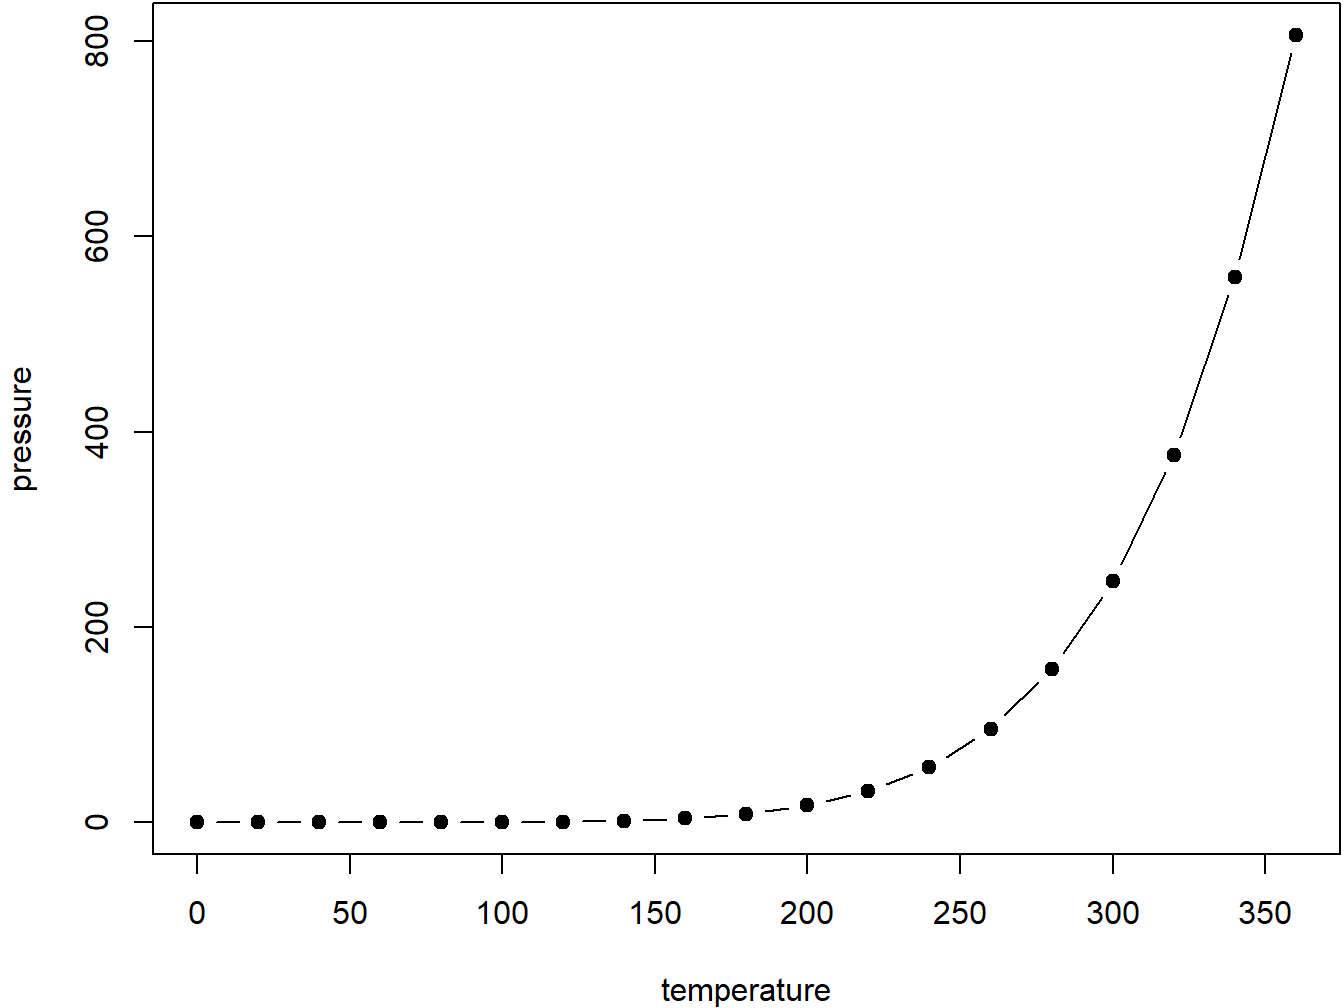
\includegraphics[width=0.8\linewidth]{bookdown_files/figure-latex/nice-fig-1} 

}

\caption{Here is a nice figure!}\label{fig:nice-fig}
\end{figure}

Reference a figure by its code chunk label with the \texttt{fig:}
prefix, e.g., see Figure \ref{fig:nice-fig}. Similarly, you can
reference tables generated from \texttt{knitr::kable()}, e.g., see Table
\ref{tab:nice-tab}.

\begin{Shaded}
\begin{Highlighting}[]
\NormalTok{knitr}\OperatorTok{::}\KeywordTok{kable}\NormalTok{(}
  \KeywordTok{head}\NormalTok{(iris, }\DecValTok{3}\NormalTok{), }\DataTypeTok{caption =} \StringTok{'Here is a nice table!'}\NormalTok{,}
  \DataTypeTok{booktabs =} \OtherTok{TRUE}
\NormalTok{)}
\end{Highlighting}
\end{Shaded}

\begin{table}

\caption{\label{tab:nice-tab}Here is a nice table!}
\centering
\begin{tabular}[t]{rrrrl}
\toprule
Sepal.Length & Sepal.Width & Petal.Length & Petal.Width & Species\\
\midrule
5.1 & 3.5 & 1.4 & 0.2 & setosa\\
4.9 & 3.0 & 1.4 & 0.2 & setosa\\
4.7 & 3.2 & 1.3 & 0.2 & setosa\\
\bottomrule
\end{tabular}
\end{table}

You can write citations, too. For example, we are using the
\textbf{bookdown} package \citep{R-bookdown} in this sample book, which
was built on top of R Markdown and \textbf{knitr} \citep{xie2015}.

\section{Marco conceptual}\label{marco}

\subsection{Análisis de correspondencias
múltiples}\label{analisis-de-correspondencias-multiples}

Como se presenta en Pardo \citep[pp.~125 - 163]{Pardo}, el análisis de
correspondencias múltiples es una herramienta estadística cuyo objetivo
es analizar asociaciones entre categorías de las variables de interés,
esto a través de métodos gráficos que permitan observar cuales
categorías de una variable son las que más afectan a las diferentes
categorías de las otras variables, además permite reducir la dimensión
de la matriz de datos de tal manera que se pueda llegar a observar las
relaciones de las categorías usando un gráfico bidimensional. Se puede
entender como un análisis de correspondencias simples aplicado a una
tabla disyuntiva completa o bien aplicado a la tabla de Burt
correspondiente teniendo en cuenta que en este caso se pierde la
información por individuo. El método, como ya se dijo, se puede entender
como la generalización de un análisis de correspondencias simple al caso
de más de dos variables categóricas de interés, pero también se puede
entender como la realización de dos diferentes análisis de componentes
principales, uno de ellos permite hacer los cálculos de una manera
relativamente sencilla y el otro ayuda a llevar a cabo la interpretación
de los ejes obtenidos, en general, esta interpretación se hace
únicamente sobre las categorías de las variables y no sobre los
individuos ya que los últimos son, en la mayoría de los casos, anónimos.
Para seleccionar el número de ejes a retener se usan dos metodologías,
la primera es elegir el número a través del histograma de valores
propios de los ejes de acuerdo a la cantidad de valores propios que se
puedan considerar diferentes, y si hay muchos valores propios similares
se considera que pertenecen a ejes ``parásitos'', es decir a ejes que no
brindan más información. La segunda metodología se conoce como el
criterio de Benzecri, dentro de los ejes cuyo valor propio sea mayor al
inverso del número de categorías dentro del análisis se recalcula las
tasas de inercia y se selecciona el número de ejes a través del
histograma de las tasas de inercia recalculadas de la misma manera que
se hizo con el histograma de valores propios. El análisis de
correspondencias múltiples permite, además, incluir la proyección de
variables que no participaron en la construcción de los ejes, a estas
variables se les conoce como suplementarias y sirve para describir las
posibles relaciones que presentan esas categorías suplementarias con las
categorías de las variables activas del análisis.

\subsection{Modelos multinomiales}\label{modelos-multinomiales}

Cuando en un problema de modelación estadística, la variable dependiente
o de respuesta es de tipo categórico nominal una de las opciones para
llevar a cabo el análisis es recurrir a modelos logit de categoría base
adecuados a respuestas de tipo nominal \citep[pp.~267]{Agresti}. Este
modelo, también conocido como modelo multinomial, es un análisis
conjunto de modelos logit binarios para cada par de categorías como se
observa en la ecuación (1):

\[\log { \left( \frac { { \pi  }_{ j } }{ { \pi  }_{ J } }  \right)  } ={ \alpha  }_{ j }+{ \beta  }_{ j }x,\quad \quad \quad j=1,\cdots ,J-1 \quad \quad(1)\]

Donde \(J\) es el número total de categórias, \(x\) es una matriz cuyas
columnas corresponden a las variables explicativas, \({ \alpha }_{ j }\)
y \({ \beta }_{ j }\) son los parámetros a estimar en el modelo y
\({ \pi }_{ j }(x)=P(Y=j|x)\) las probabilidades asociadas a cada una de
las categorías de la variable respuesta \(Y\) con
\(\sum _{ j=1 }^{ J }{ { \pi }_{ j }(x) } =1\). Nótese que se puede
hallar la asociación de cualquier par de categorías a través de la
ecuación (2):

\[\log { \left( \frac { { \pi  }_{ a } }{ { \pi  }_{ b } }  \right)  } =\log { \left( \frac { { \pi  }_{ a } }{ { \pi  }_{ J } }  \right)  } -\log { \left( \frac { { \pi  }_{ b } }{ { \pi  }_{ J } }  \right)  } \quad \quad (2)\]

Para llevar a cabo la comparación entre modelos y poder seleccionar el
más adecuado, en términos de cuáles son las variables que lo van a
conformar y de la parsimonia del modelo, se usa el AIC o criterio de
información de Akaike, el cual evalúa al modelo de acuerdo a la cercanía
entre los valores ajustados a través del modelo y los verdaderos valores
penalizando por el número de parámetros \citep[pp.~216]{Agresti} y
permite comparar el ajuste de modelos que no están anidados. Cuando se
usa el AIC el modelo que más se ajusta a los datos será aquel que tenga
menor AIC y también se usa el BIC o criterio de información bayesiano,
el cual es muy similar al AIC, pero además toma en cuenta el tamaño de
la muestra \citep[pp.~257]{Agresti}. El proceso que se lleva a cabo para
la selección del modelo se conoce como backward o eliminación hacia
atrás, y se conduce como en \citet[ pp.~214]{Agresti}, es decir se parte
del modelo más completo y se elimina un parámetro a la vez. Para llevar
a cabo la estimación de las probabilidades de respuesta a través del
modelo se aplica la fórmula (3):

\[{ \hat { \pi  }  }_{ j }(x)=\frac { exp({ \hat { \alpha  }  }_{ j }+{ \hat { \beta ' }  }_{ j }x) }{ 1+\sum _{ h=1 }^{ J-1 }{ exp({ \hat { \alpha  }  }_{ h }+{ \hat { \beta ' }  }_{ h }x) }  } \quad \quad (3)\]

Y como se observa en la ecuación (4), los parámetros se pueden
interpretar a través del logit de una probabilidad condicional:

\[\log { \left( \frac { { \pi  }_{ j } }{ { \pi  }_{ J } }  \right)  } =\log { \left( \frac { \left( \frac { { \pi  }_{ j } }{ { \pi  }_{ J }+{ \pi  }_{ j } }  \right)  }{ \left( \frac { { \pi  }_{ J } }{ { \pi  }_{ J }+{ \pi  }_{ j } }  \right)  }  \right)  } =\log { \left( \frac { \left( \frac { { \pi  }_{ j } }{ { \pi  }_{ J }+{ \pi  }_{ j } }  \right)  }{ 1-\left( \frac { { \pi  }_{ j } }{ { \pi  }_{ J }+{ \pi  }_{ j } }  \right)  }  \right)  } =logit\left( \frac { { \pi  }_{ j } }{ { \pi  }_{ J }+{ \pi  }_{ j } }  \right) \quad \quad (4)\]

\subsection{Modelos multinomiales logísticos
multinivel}\label{modelos-multinomiales-logisticos-multinivel}

Los modelos multinivel aparecen, principalmente, en aplicaciones de la
estadística para hacer análisis con respecto a la educación
\citep{Goldstein}. Surgen como una ampliación a los modelos
generalizados ya existentes, para los cuales uno de sus supuestos
básicos es la independencia de las observaciones, pero al observar que
los individuos que se están analizando se encuentran agrupados
(estudiantes dentro de salones, salones dentro de colegios, etc\ldots{})
y que dentro de los grupos los individuos, en general, son similares
pero entre grupos existen diferencias más claras, es decir, se viola el
supuesto de independencia los modelos existentes ya no son válidos en
este caso. En términos simples, el modelo multinivel hace una corrección
al problema de independencia a través de la inclusión de variables
aleatorias correspondientes a los múltiples niveles de anidación de
nuestros datos y que permiten llevar cabo estimaciones correctas de los
parámetros del modelo. Para nuestro caso el modelo de interés es de
respuesta categórica nominal, de ahí que el modelo a usar resulte un
modelo multinomial logístico multinivel \citep{Goldstein} de manera en
que se especifica en la fórmula (5):

\[\log { \left( \frac { { { \pi  }_{ j } }^{ (s) } }{ { { \pi  }_{ J } }^{ (s) } }  \right)  } ={ \alpha  }_{ j }+{ \beta  }_{ j }{ x }^{ (s) }+{ { u }_{ j } }^{ (s) },\quad \quad \quad j=1,\cdots ,J-1\quad \quad (5)\]

Donde \(J\) es el número total de categórias, x es una matriz cuyas
columnas corresponden a las variables explicativas, \({ \alpha }_{ j }\)
y \({ \beta }_{ j }\) son los parámetros a estimar en el modelo, \(s\)
es el nivel de agrupación de las observaciones y
\({ { \pi }_{ j } }^{ (s) }({ x }^{ (s) })=P(Y=j|{ x }^{ (s) },s)\) las
probabilidades asociadas a cada una de las categorías de la variable
respuesta Y en cada uno de los niveles (\(S\)),
\(\sum _{ j=1 }^{ J }{ \sum _{ s=1 }^{ S }{ { { \pi }_{ j } }^{ (s) }(x) } } =1\)
y el \({ { u }_{ j } }^{ (s) }\) es un error aleatorio asociado a cada
nivel. Se tienen como opciones la cuasi verosimilitud, la máxima
verosimilitud o los procedimientos MCMC para la estimación de los
parámetros. Pero como se presenta en \citep{HadfieldBook}:

\emph{``En el contexto de los modelos lineales generalizados mixtos
(GLMM), aquí está lo que yo observo como los pros y los contras de usar
máxima verosimilitud (restringida - REML) versus los métodos bayesianos
de Cadenas de Markov de Monte Carlo (MCMC). REML son rápidos y fáciles
de usar, mientras los métodos MCMC pueden ser lentos y más retadores
técnicamente. En particular, el reto es la especificación de una apiori
sensible, el cual no es una dificultad con REML. Sin embargo, los
resultados analíticos para GLMM no Gaussianos en general no están
disponibles y REML se basa en procedimientos que usan métodos de máxima
verosimilitud aproximada que pueden no funcionar bien. MCMC también es
una aproximación, pero la exactitud de la aproximación incrementa en la
misma medida que aumenta la longitud del análisis, siendo exactos al
límite. Adicionalmente REML usa teoría de grandes muestras para derivar
las aproximaciones de los intervalos de confianza los cuales pueden ser
muy pobres especialmente para las varianzas. Nuevamente, las medidas de
confianza de MCMC son exactas, excepto por el error de Monte Carlo, y
proveen de una manera fácil e intuitiva de obtener medidas de confianza
derivadas de las estadísticas como las razones de varianza,
correlaciones y predicciones.''}

Luego para tamaños de muestra grandes y siempre que los métodos
computacionales estén disponibles se puede acudir a métodos de
estimación REML, en los demás casos la solución será acudir a métodos de
estimación MCMC. Para más detalles sobre la estimación de parámetros de
los modelos multinivel desde la perspectiva frecuentista de los modelos
multinivel véase (Goldstein, 2010) y para la estimación de los
parámetros desde la perspectiva bayesiana véase \citep{Goldstein} y/o
\citep{HadfieldBook}. Para validar los supuestos y ajuste de los modelos
multinivel existen dos caminos a seguir y dependen de la manera en que
decidamos hacer la estimación de los parámetros de nuestro modelo. En la
primera manera, es decir, la frecuentista o REML los supuestos son: en
primera medida que los datos provengan de la distribución de
probabilidades teorizada por el modelo, pero a diferencia de los modelos
lineales generalizados usuales, los modelos multinivel no requieren la
independencia de los errores. En la segunda manera, es decir, la
bayesiana o MCMC los supuestos son: que los datos provengan de la
distribución de probabilidades teorizada por el modelo, que la
distribución a priori (que puede, o no, ser informativa) conjugue con la
función de máxima verosimilitud de los datos, además se debe verificar
que las cadenas de Márkov converjan para la estimación de los
parámetros. Al llevar a cabo las verificaciones anteriormente descritas
y apropiadas al método usado para la estimación entonces se garantiza
que nuestro modelo ha sido validado y que el mismo se ha ajustado a
nuestros datos.

\subsection{Software estadístico R:}\label{software-estadistico-r}

R es un leguaje y ambiente de computación estadístico de código libre
(GNU project) construido para dar sentido y valor agregado a los datos.
R provee de una muy amplia variedad de herramientas estadísticas la cual
es alimentada por su activa y creciente comunidad de colaboradores y
usuarios. RStudio es una IDE (entorno de desarrollo integrado) para R,
la comunidad de desarrolladores de RStudio inspirados por las
innovaciones de los usuarios de R en las ciencias, educación e industria
desarrollaron gran cantidad de herramientas, la mayoría libres, que
permite dar gran valor añadido a los datos (dashboards, htmlwidgets,
libros, etc\ldots{}) y para que los equipos de trabajo puedan promover y
compartir el trabajo posicionando a R como el lenguaje estadístico, de
inteligencia de negocios y de ciencia de datos más poderoso, innovador y
de mayor crecimiento en el mundo. Entre la gran variedad de librerías
que posee R describiremos a continuación aquellas que fueron utilizadas
en el desarrollo del proyecto. \textbf{Referencias:} \citep{r1},
\citep{wikiR}, \citep{wikiRStudio}, \citep{rstudio1}, \citep{rstudio2}.

\subsubsection{Librería tidyverse:}\label{libreria-tidyverse}

Es una colección de paquetes de R diseñados para ciencia de datos. Todos
los paquetes comparten una filosofía de diseño subyacente, gramática y
estructuras de datos. Contiene ggplot2 la cual es una librería poderosa
para hacer gráficos estáticos por capas, dplyr la cual sirve para la
manipulación de datos, tidyr la cual ayuda a depurar las bases de datos,
readr para la lectura de datos rectangulares, readxl para la lectura de
archivos .xls y .xlsx, purrr la cual permite hacer programación
funcional, tibble la cual es una manera moderna de pensar las
estructuras de datos, stringr la cual se encarga de que el trabajo con
caracteres (strings) sea lo más sencillo posible, forcats la cual
permite solucionar problemas frecuentes con la manipulación de factores,
entre otros muchos paquetes. \textbf{Referencias:} \citep{tidyverse}

\subsubsection{Librería Factoclass:}\label{libreria-factoclass}

Como lo describe dos de sus autores Campo Elías Pardo (profesor asociado
del Departamento de Estadística de la Universidad Nacional de Colombia)
y Pedro César del Campo (Estadístico de la Universidad Nacional de
Colombia) en \citep{Pardo2007}, el paquete se implementó con la
finalidad de llevar a cabo exploración multivariada de datos de acuerdo
con las estrategias descritas en \citep{Lebart} . \textbf{Referencias:}
\citep{Factoclass}

\subsubsection{Librería lme4:}\label{libreria-lme4}

Es una librería construida para el ajuste de modelos lineales de efectos
mixtos y modelos lineales generalizados de efectos mixtos desde un
enfoque de máxima verosimilitud restringida. \textbf{Referencias:}
\citep{lme4}, \citep{Bates}

\subsubsection{Librería MCMCglmm:}\label{libreria-mcmcglmm}

Es una librería de R la cual tiene como objetivo ajustar modelos
lineales generalizados mixtos con un enfoque bayesiano a través del uso
de Cadenas de Markov Monte Carlo (MCMC). \textbf{Referencias:}
\citep{MCMCglmm}, \citep{HadfieldBook}, \citep{HadfieldCourseNotes}.

\section{Metodología}\label{metodologuxeda}

La metodología llevada a cabo se divide en hacer análisis para los
estudiantes PAES y para los estudiantes PEAMA, que ingresaron en la
cohorte 2011-01, por separado. La metodología en ambos casos es la misma
y consta de los siguientes pasos:

\begin{enumerate}
\def\labelenumi{\arabic{enumi}.}
\tightlist
\item
  Construcción descriptiva univariada del panorama de admisión de cada
  una de las dos poblaciones (PEAMA y PAES).
\item
  Revisión de la normatividad existente al ingreso de los dos grupos y
  su posterior validación.
\item
  Construcción de análisis de correspondencias múltiples para las
  variables incluidas en la permanencia y graduación que permita
  comprender como se relacionan los diferentes desenlaces con las
  varibales que pertenecen a los estudiantes al momento de admisión, las
  variables en su proceso académico y su participación en programas de
  bienestar, para cada uno de los dos grupos de estudiantes (PAES y
  PEAMA).
\end{enumerate}

También se va a llevar a cabo un análisis de proceso para el programa
PEAMA Tumaco y para el programa PAES Victimas del conflicto armado el
cual consta de:

\section{Admisión PAES}\label{admision-paes}

En este capítulo se presenta una descripción del panorama general de
admisión de los estudiantes PAES de la cohorte 2011-01.

En primer lugar se observa cuales fueron los programas PAES por los que
los aspirantes fueron admitidos:

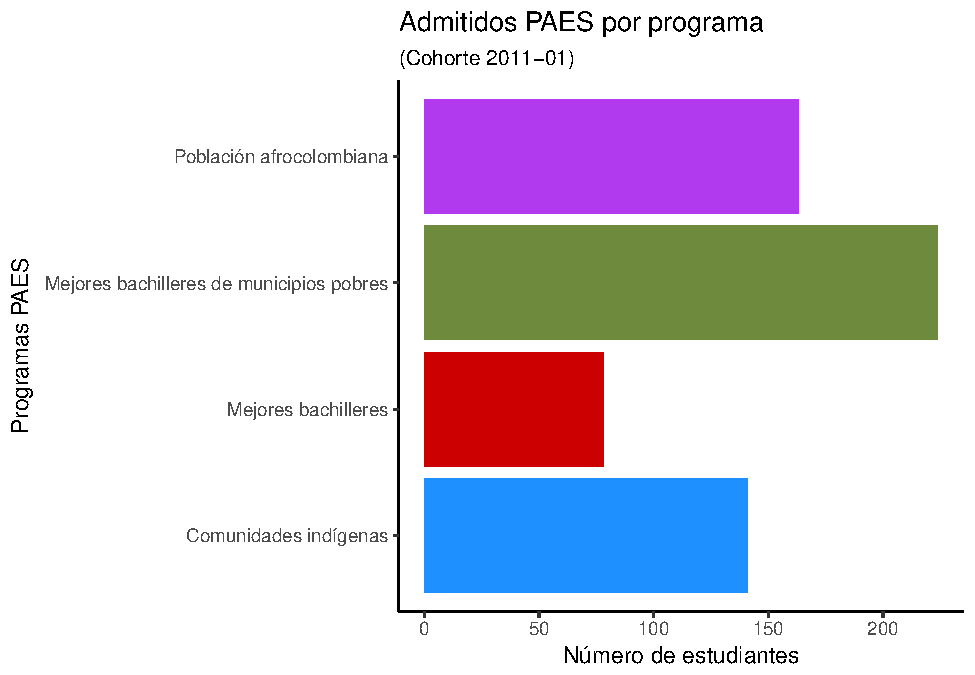
\includegraphics{bookdown_files/figure-latex/unnamed-chunk-2-1.pdf}

Observamos que la mayor parte entran por el programa \emph{mejores
bachilleres de municipios pobres} con 224 admitidos, seguido por las
\emph{poblaciones negras, afrocolombianas, palenqueras y raizales} con
163 admitidos, en tercer lugar las \emph{comunidades indígenas} con 141
admitidos y finalmente los \emph{mejores bachilleres} en último lugar
con 78 admitidos.

\subsection{Sexo de los admitidos}\label{sexo-de-los-admitidos}

Donde se encuentra que aproximadamente la tercera parte de la población
admitida como estudiantes PAES es mujer y que los restantes son hombres.
Se observa que esto ocurre además para todos los PAES de manera global y
desagregado por los programas de admisión.

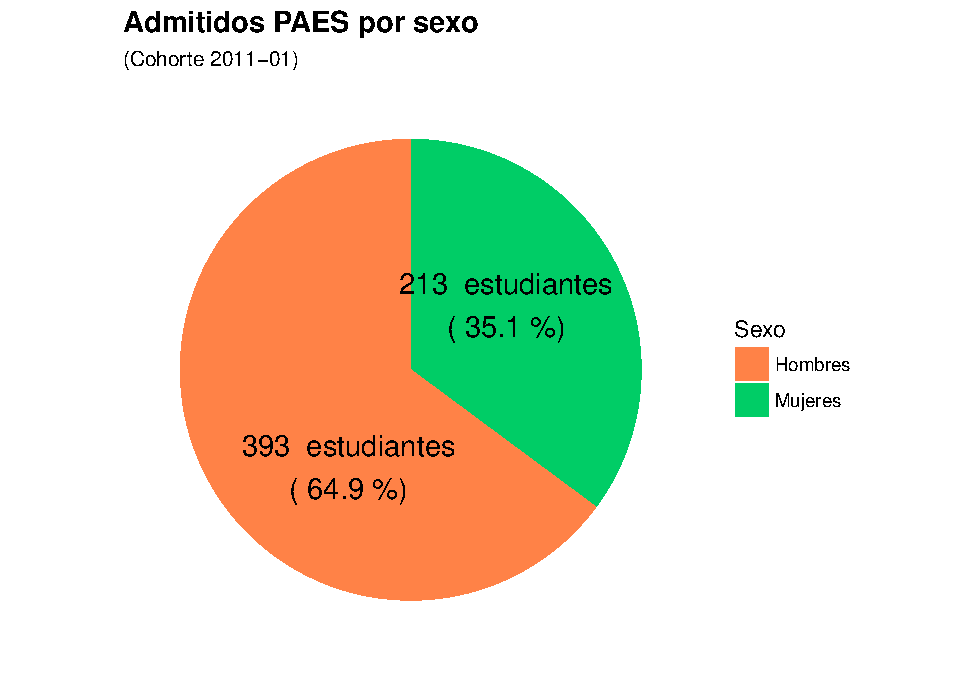
\includegraphics{bookdown_files/figure-latex/unnamed-chunk-3-1.pdf}
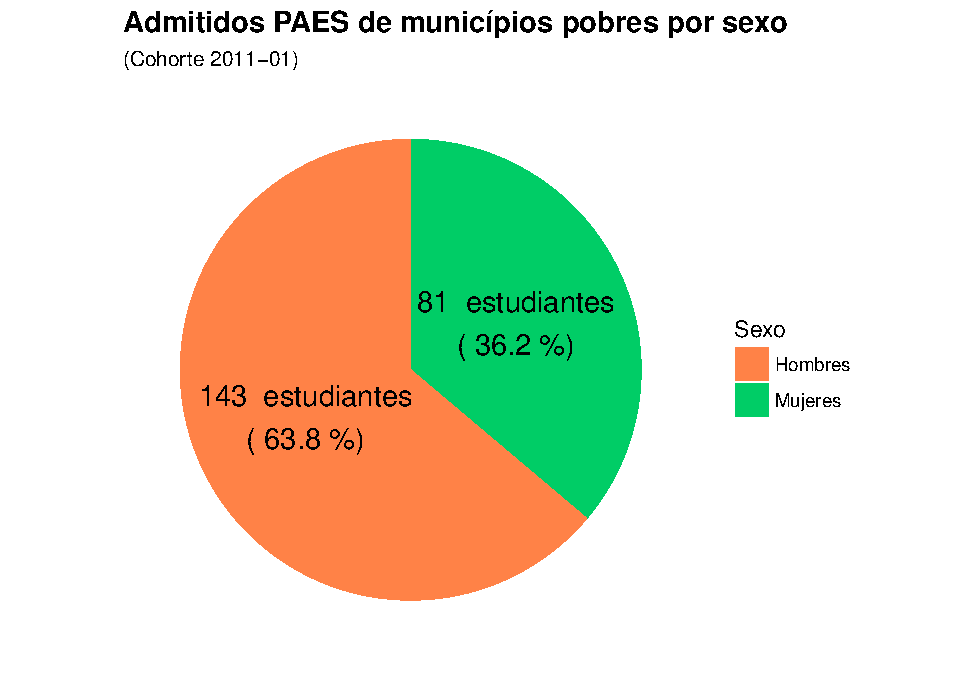
\includegraphics{bookdown_files/figure-latex/unnamed-chunk-3-2.pdf}
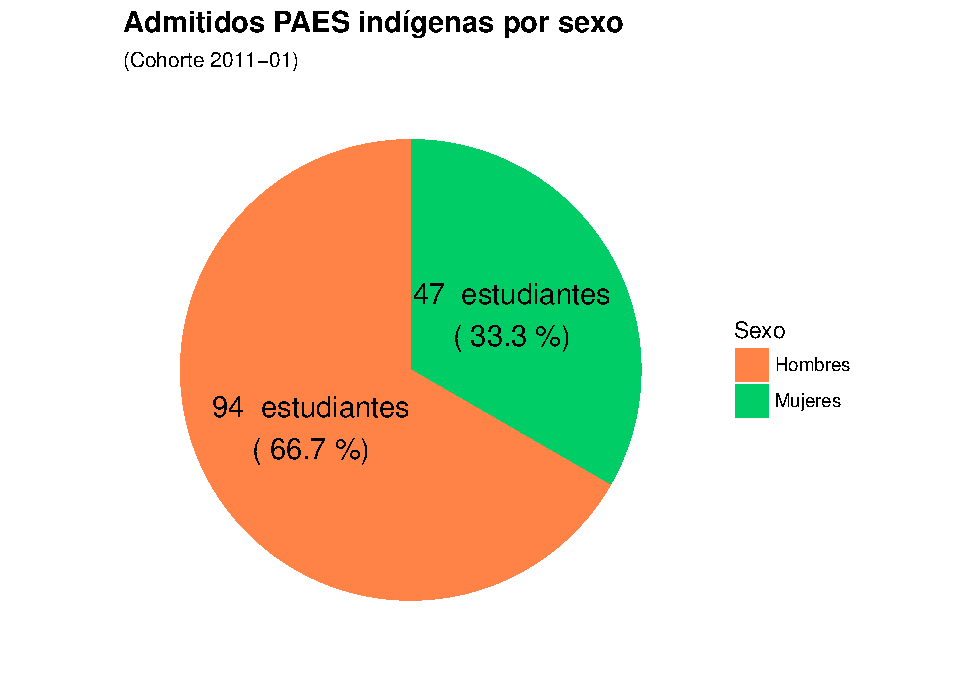
\includegraphics{bookdown_files/figure-latex/unnamed-chunk-3-3.pdf}
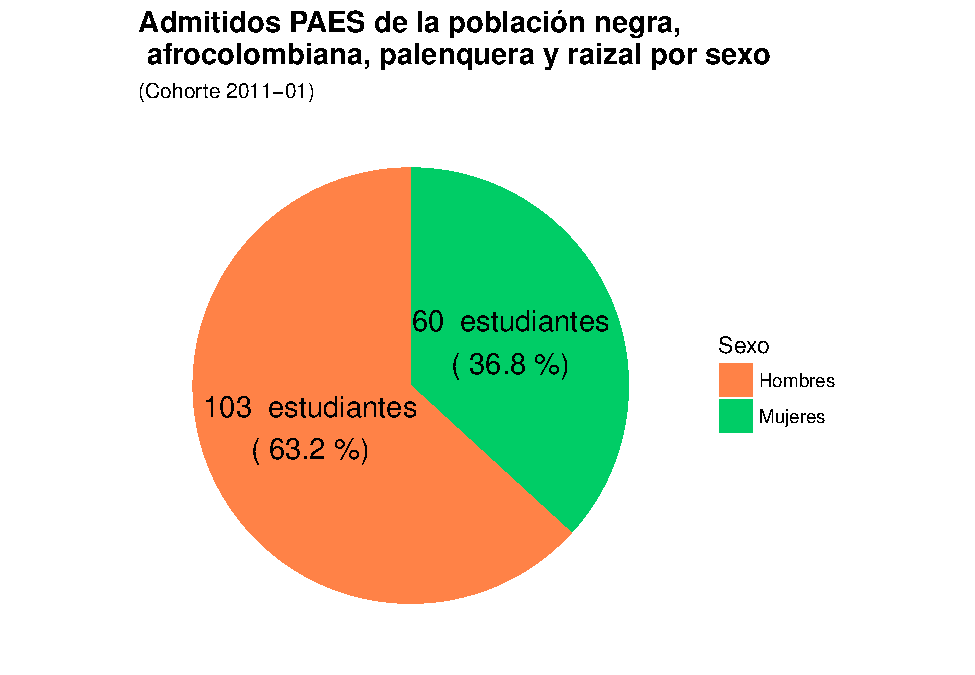
\includegraphics{bookdown_files/figure-latex/unnamed-chunk-3-4.pdf}
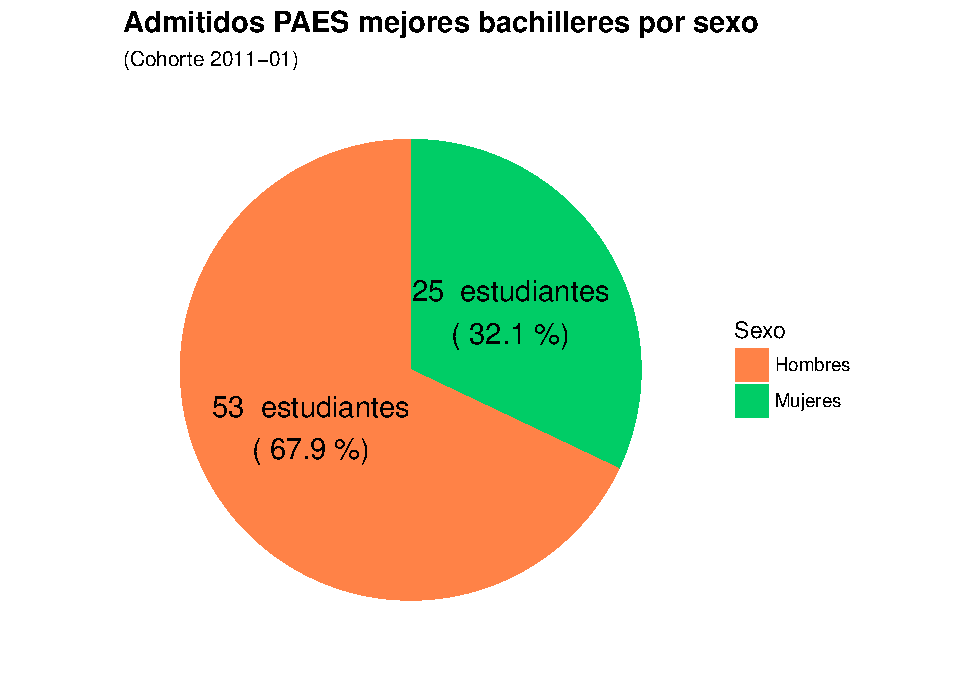
\includegraphics{bookdown_files/figure-latex/unnamed-chunk-3-5.pdf}

\subsection{Edad de los admitidos}\label{edad-de-los-admitidos}

Se haya que los estudiantes PAES admitidos tienen edades que se acumulan
principalmente entre los 16 y los 21 años siendo similar en todos los
grupos, se observa además que los grupos indígenas son los que tienen
más estudiantes en grupos de más edad (superiores a los 25 años).

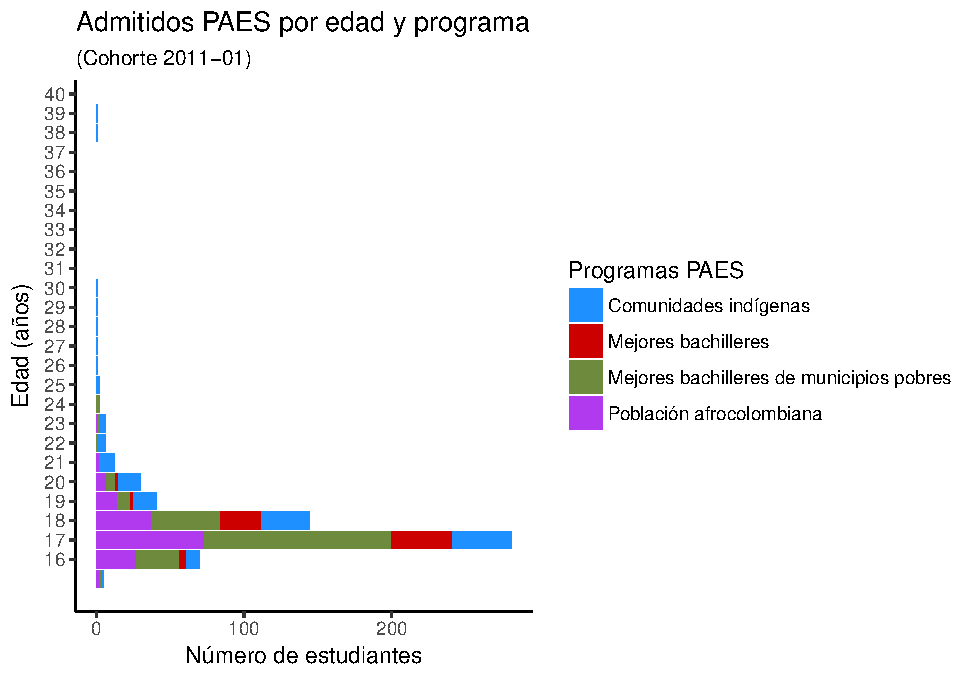
\includegraphics{bookdown_files/figure-latex/unnamed-chunk-4-1.pdf}
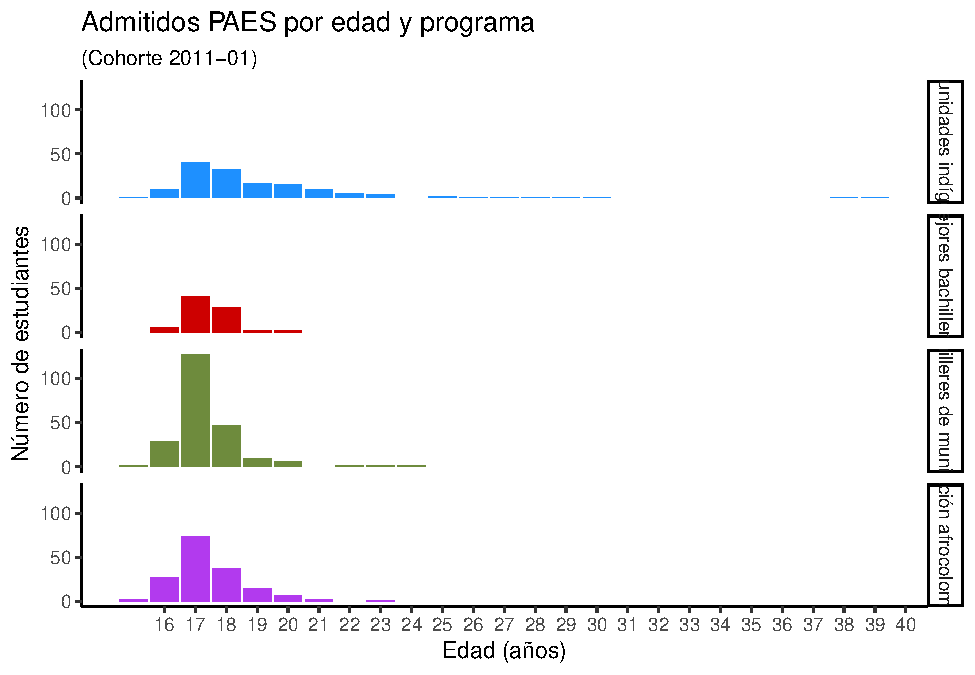
\includegraphics{bookdown_files/figure-latex/unnamed-chunk-4-2.pdf}
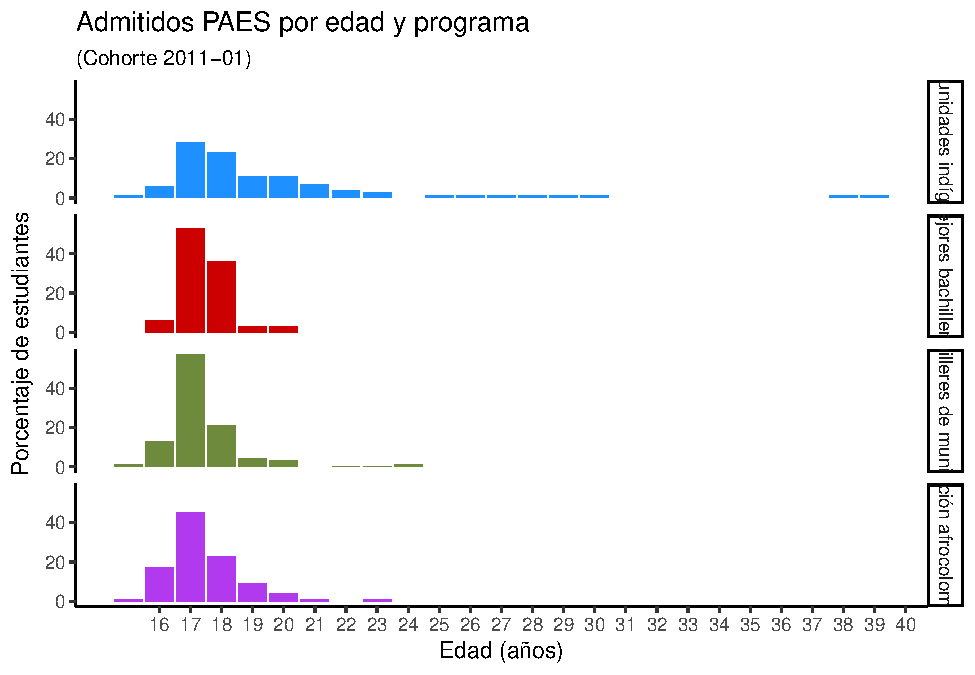
\includegraphics{bookdown_files/figure-latex/unnamed-chunk-4-3.pdf}

\subsection{Sede andina de los
admitidos}\label{sede-andina-de-los-admitidos}

Se observa que aproximadamente la mitad de los estudiantes PAES son
admitidos a la sede Bogotá, aproximadamente una cuarta parte son
admitidos a la sede Medellín y luego son admitidos a la sede Palmira y
finalmente a la sede Manizales, en cada caso con aproximadamente el 12\%
en cada caso.

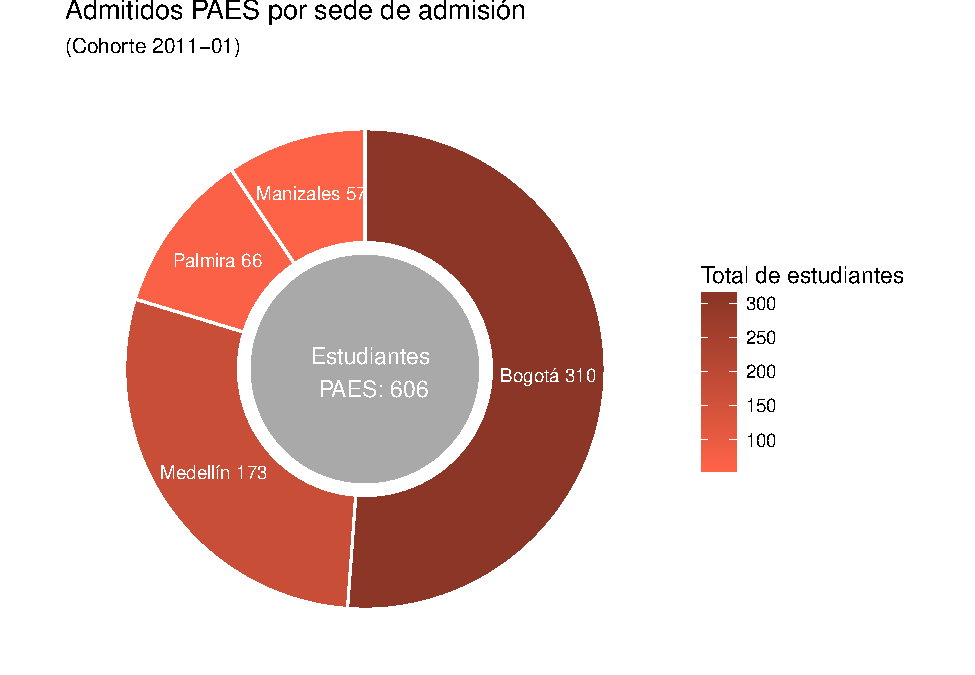
\includegraphics{bookdown_files/figure-latex/unnamed-chunk-5-1.pdf}

\subsection{Sede andina y programa de los
admitidos}\label{sede-andina-y-programa-de-los-admitidos}

Se presenta a continuación los admitidos PAES por sede y por programa.
Se encuentra que el máximo número de admitidos en algún programa es de
15 estudiantes y ocurre para el programa curricular de Administración de
Empresas de la sede de Palmira. Observamos que las cinco carreras con
más admitidos son: Palmira Administración de Empresas (15 estudiantes),
Bogotá Ingeniería Eléctrica (14 estudiantes), Bogotá Química (13
estudiantes), Palmira Ingeniería Agroindustrial y Palmira Ingeniería
Ambiental (ambas con 12 estudiantes).

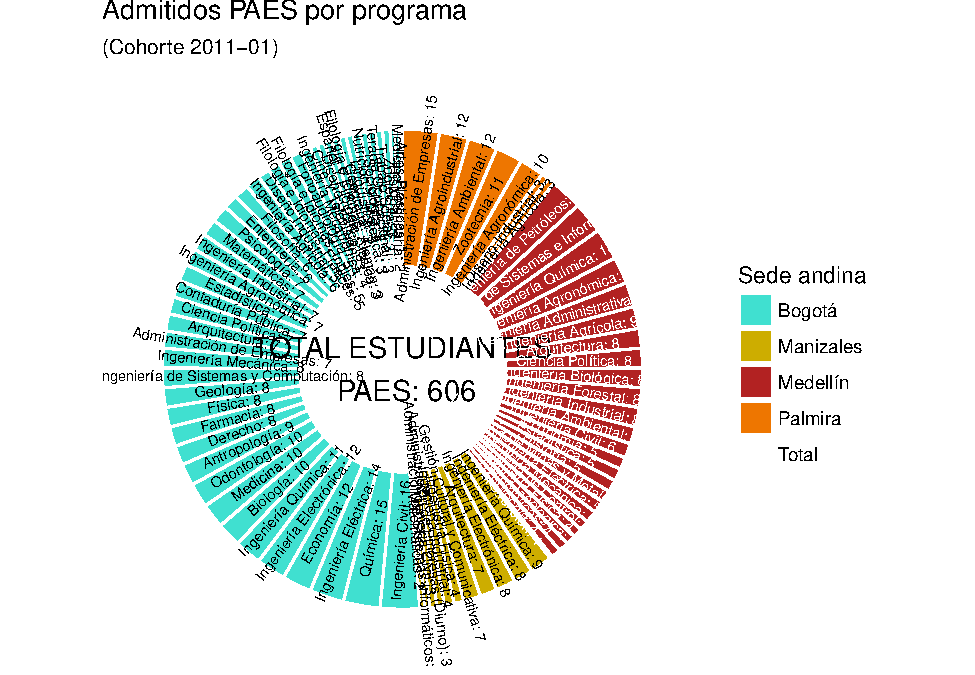
\includegraphics{bookdown_files/figure-latex/unnamed-chunk-6-1.pdf}

\subsection{Sede andina y facultad de los
admitidos}\label{sede-andina-y-facultad-de-los-admitidos}

Se hace la misma descripción anterior a los estudiantes PAES pero por
sede y facultad encontrándose que la mayor facultad con estudiantes
admitidos es la de Minas en Medellín (74 estudiantes), seguida por
Ingeniería Bogotá (65 estudiantes), Ciencias Bogotá (52 estudiantes),
Ingeniería y Administración Palmira (45 estudiantes), Ciencias Humanas
Bogotá (44 estudiantes) e Ingeniería y Administración Manizales (37
estudiantes), donde se observa un gran interés principalmente por la
ingeniería en los admitidos PAES.

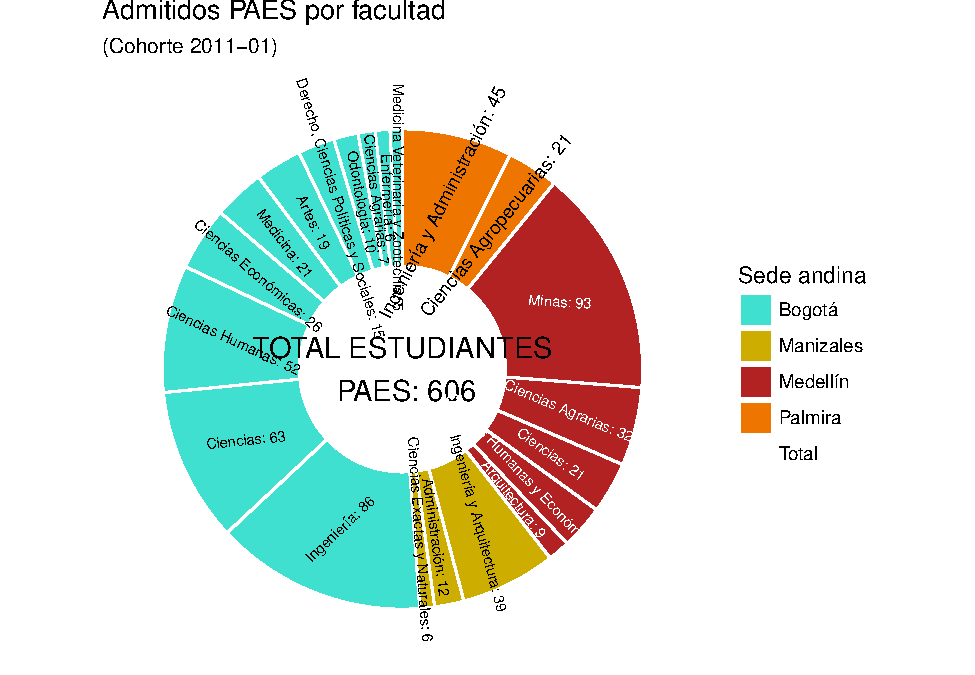
\includegraphics{bookdown_files/figure-latex/unnamed-chunk-7-1.pdf}

\subsection{Estrato socioeconómico de los
admitidos}\label{estrato-socioeconomico-de-los-admitidos}

Se hace la misma descripción anterior a los estudiantes PAES pero por
sede y facultad encontrándose que la mayor facultad con estudiantes
admitidos es la de Minas en Medellín (74 estudiantes), seguida por
Ingeniería Bogotá (65 estudiantes), Ciencias Bogotá (52 estudiantes),
Ingeniería y Administración Palmira (45 estudiantes), Ciencias Humanas
Bogotá (44 estudiantes) e Ingeniería y Administración Manizales (37
estudiantes), donde se observa un gran interés principalmente por la
ingeniería en los admitidos PAES.

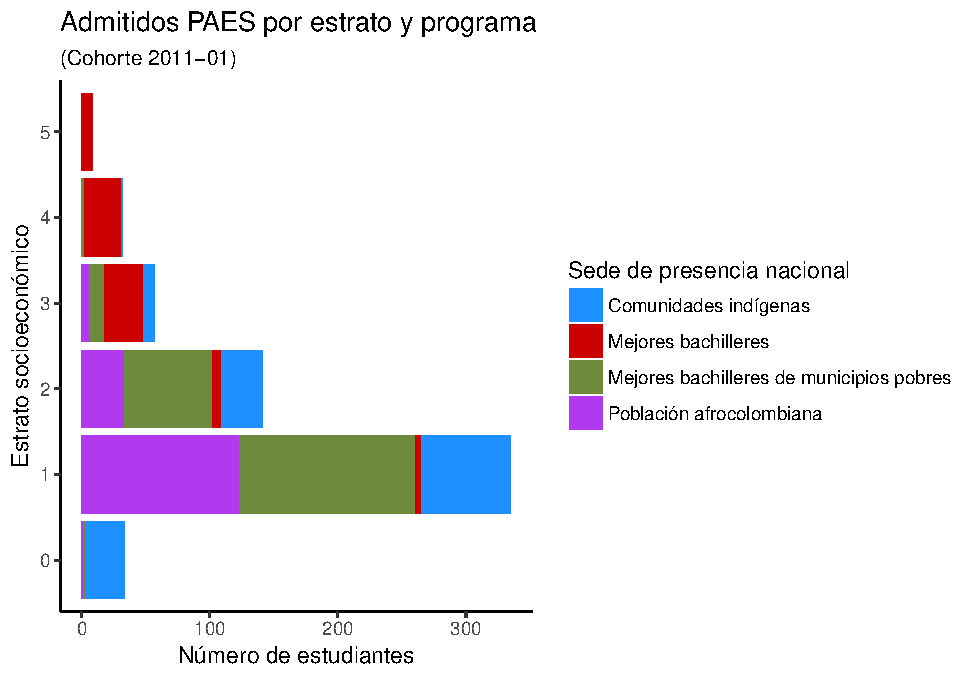
\includegraphics{bookdown_files/figure-latex/unnamed-chunk-8-1.pdf}
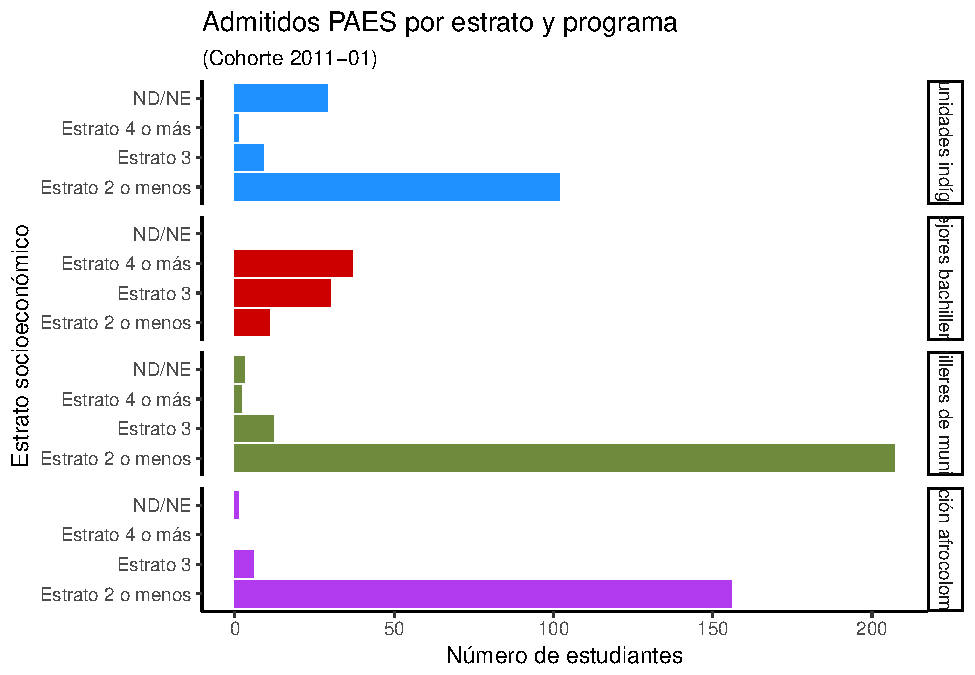
\includegraphics{bookdown_files/figure-latex/unnamed-chunk-8-2.pdf}
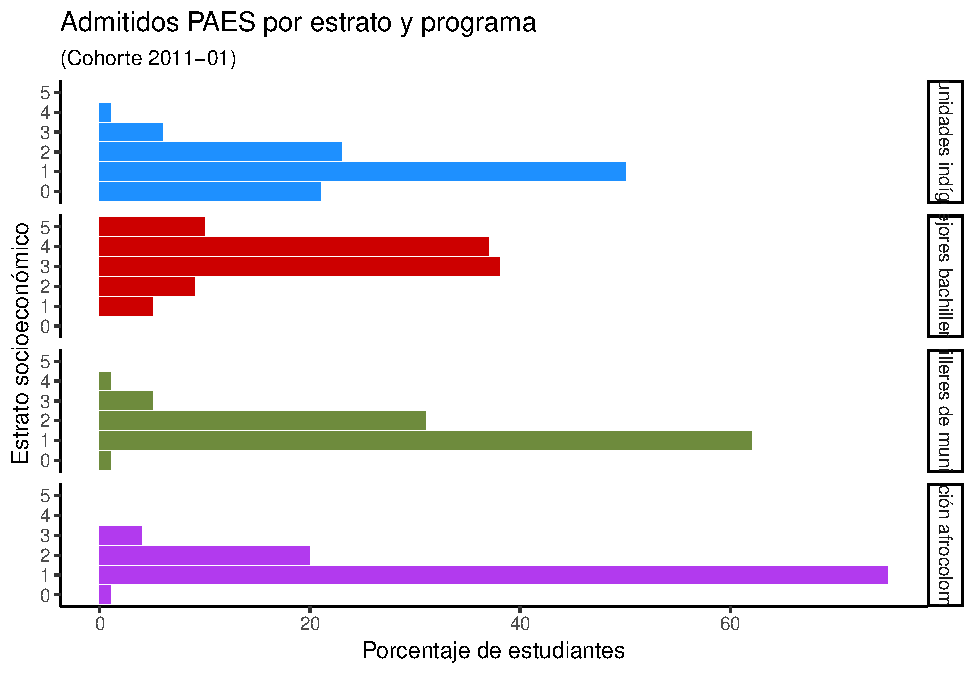
\includegraphics{bookdown_files/figure-latex/unnamed-chunk-8-3.pdf}

\subsection{Puntaje en examen de
admisión}\label{puntaje-en-examen-de-admision}

Se observa que los mayores puntajes de admisión los presentan los
estudiantes PAES correspondientes a los mejores bachilleres de
municipios pobres (con una mediana de 575,1268), seguido por los PAES
indigenas (mediana de 533.4272) y finalmente los PAES afrocolombianos,
palenqueros y raizales (mediana de 520.6273). Se observa además (en
rojo) el puntaje de admisión del último admitido de manera regular y se
encuentra que los estudiantes PAES tienen puntajes de admisión que son
iguales o superiores a ese puntaje (451,2525).

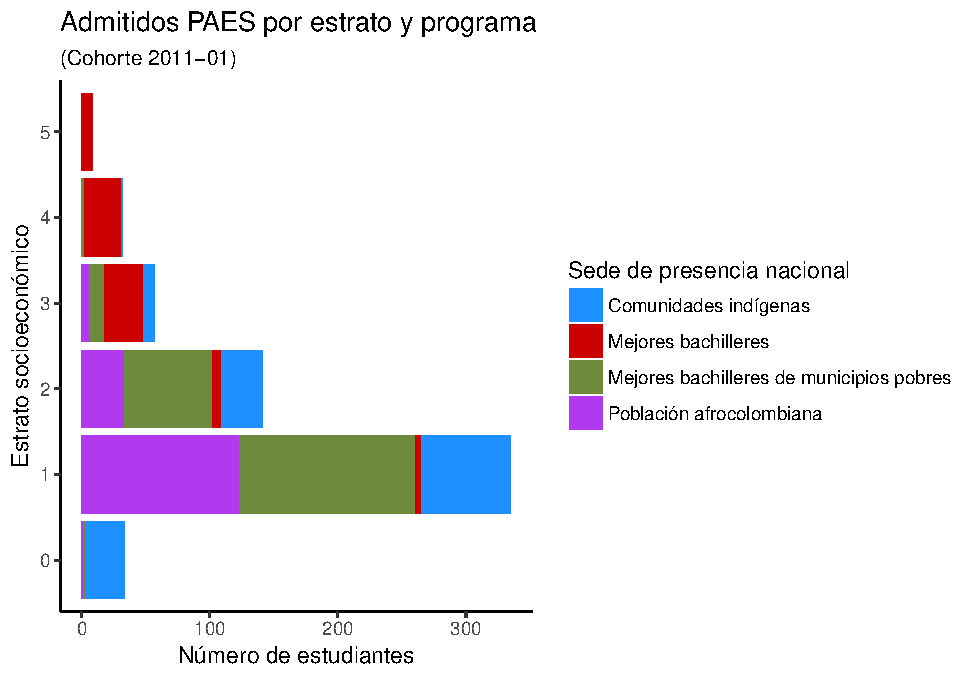
\includegraphics{bookdown_files/figure-latex/unnamed-chunk-9-1.pdf}

\subsection{Porcentaje de admitidos v.s. total de
aspirantes}\label{porcentaje-de-admitidos-v.s.-total-de-aspirantes}

Si comparamos a los admitidos con los aspirantes para cada programa
curricular y programa PAES obtenemos el porcentaje de admisión, que
también se puede ver como un índice de absorción específico. En el caso
de la sede Bogotá y de la sede Manizales se tiene que los porcentajes de
admisión dentro de los programas especiales de admisión son mayores
comparados con los porcentajes de admisión para los admitidos regulares,
excepto por unos pocos casos.

No ocurre lo mismo para las sedes Medellín y Palmira, en el primero se
tienen muchos casos donde la porcentaje de admitidos es mayor en los
programas PAES comparados con los regulares, así mismo se tienen muchos
casos donde el porcentaje de admitidos regulares es mayor comparado con
el de admitidos PAES por programa. En el caso de la sede Palmira se
observa que en la mayoría de casos los admitidos por programa tienen una
mayor proporción comparados con la proporción que existe dentro de cada
uno de los programas PAES.

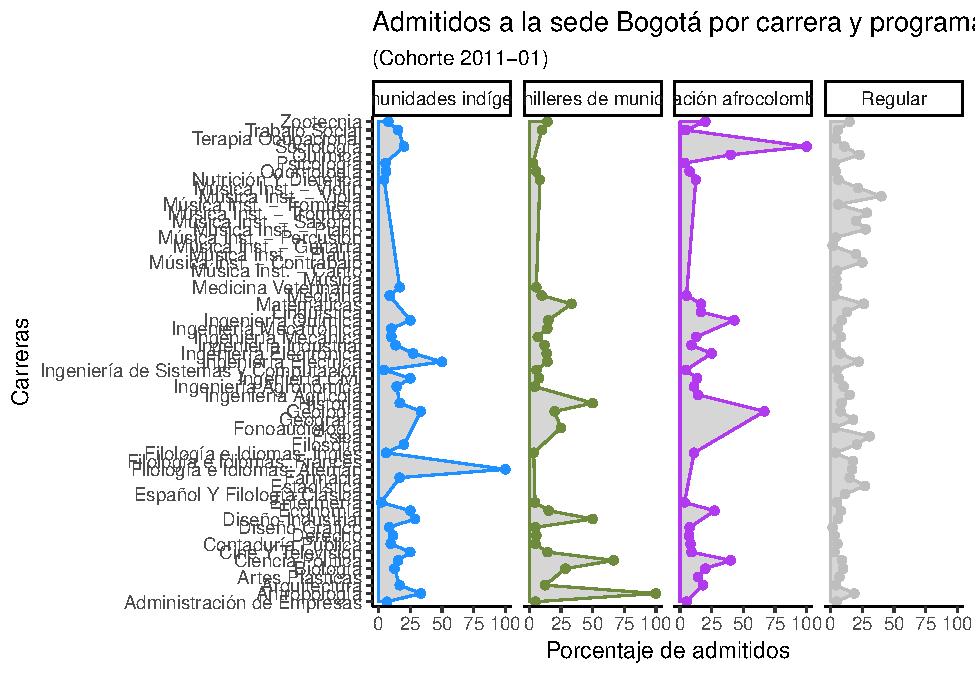
\includegraphics{bookdown_files/figure-latex/unnamed-chunk-10-1.pdf}
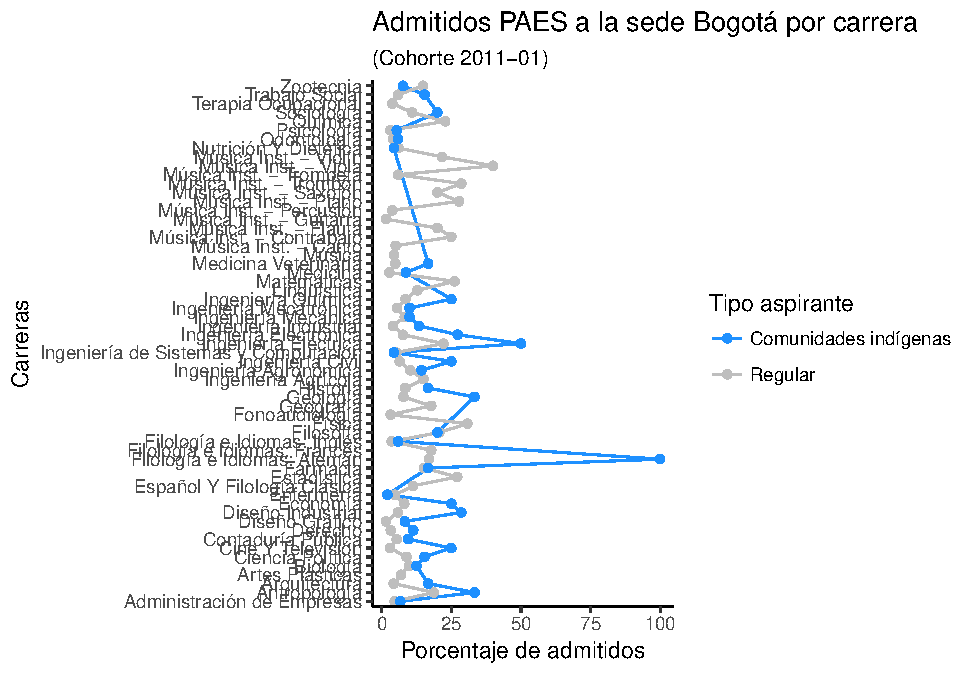
\includegraphics{bookdown_files/figure-latex/unnamed-chunk-10-2.pdf}
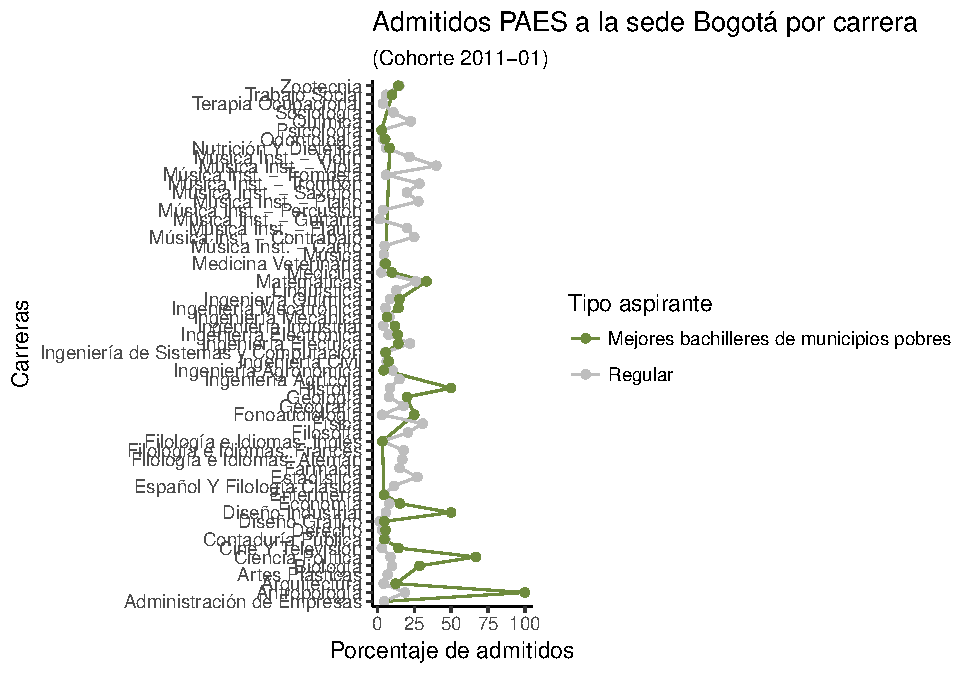
\includegraphics{bookdown_files/figure-latex/unnamed-chunk-10-3.pdf}
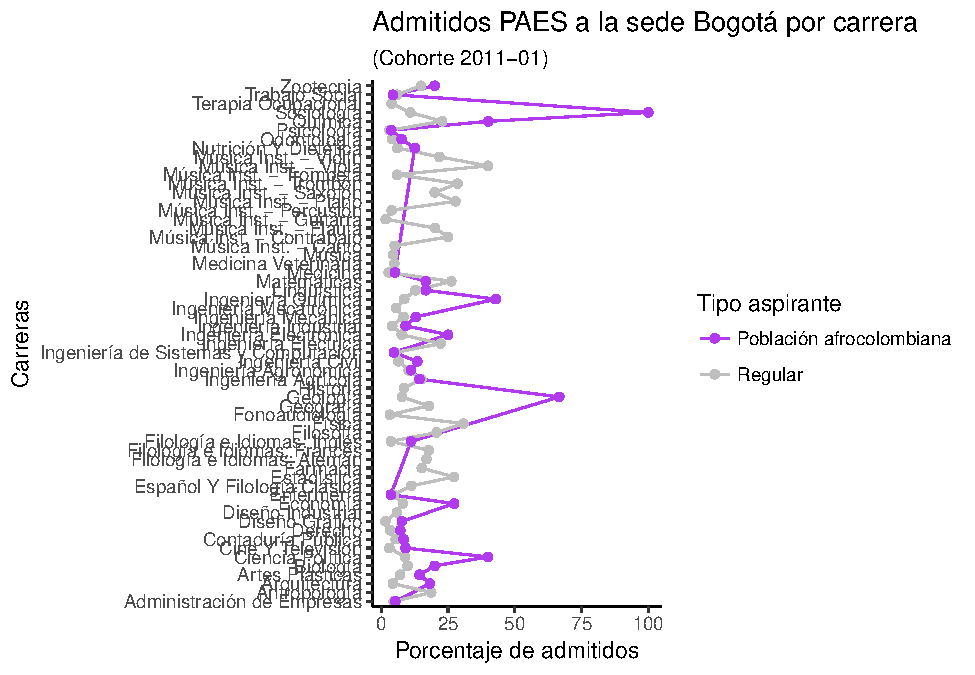
\includegraphics{bookdown_files/figure-latex/unnamed-chunk-10-4.pdf}

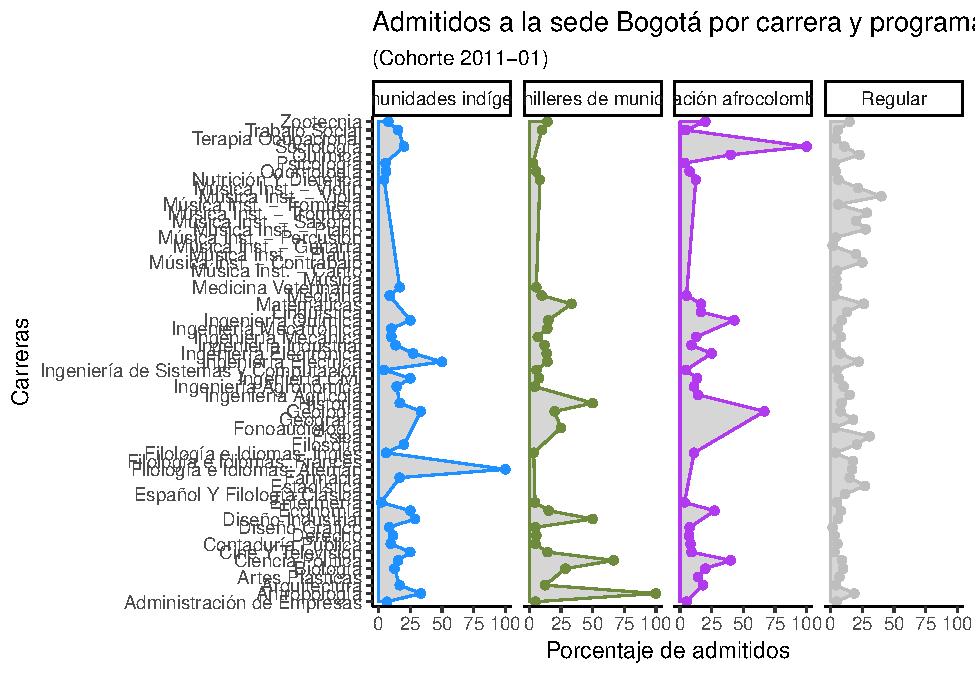
\includegraphics{bookdown_files/figure-latex/unnamed-chunk-11-1.pdf}
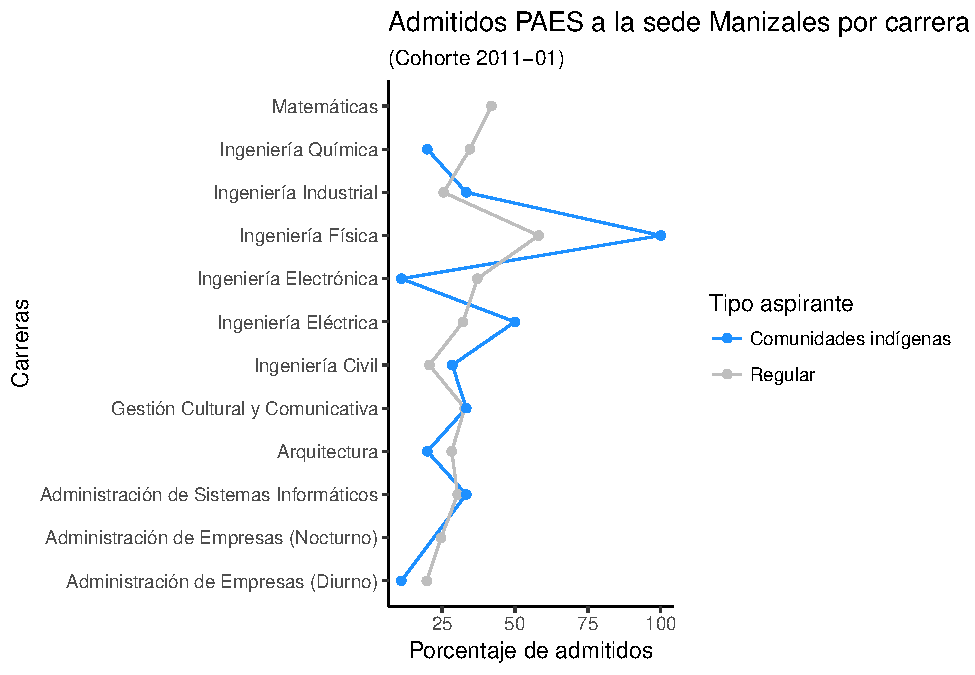
\includegraphics{bookdown_files/figure-latex/unnamed-chunk-11-2.pdf}
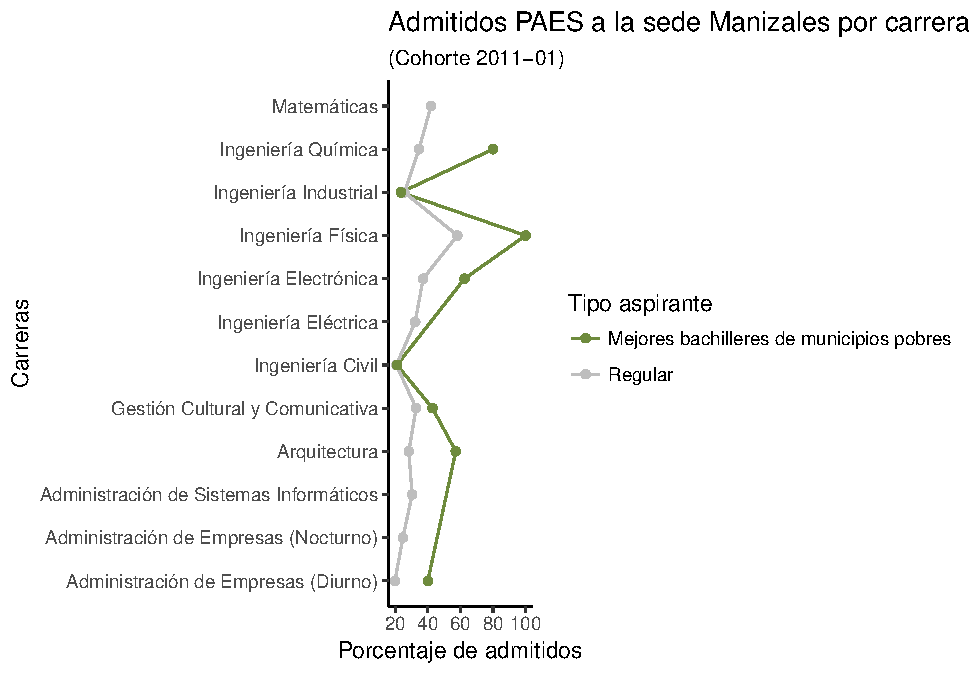
\includegraphics{bookdown_files/figure-latex/unnamed-chunk-11-3.pdf}
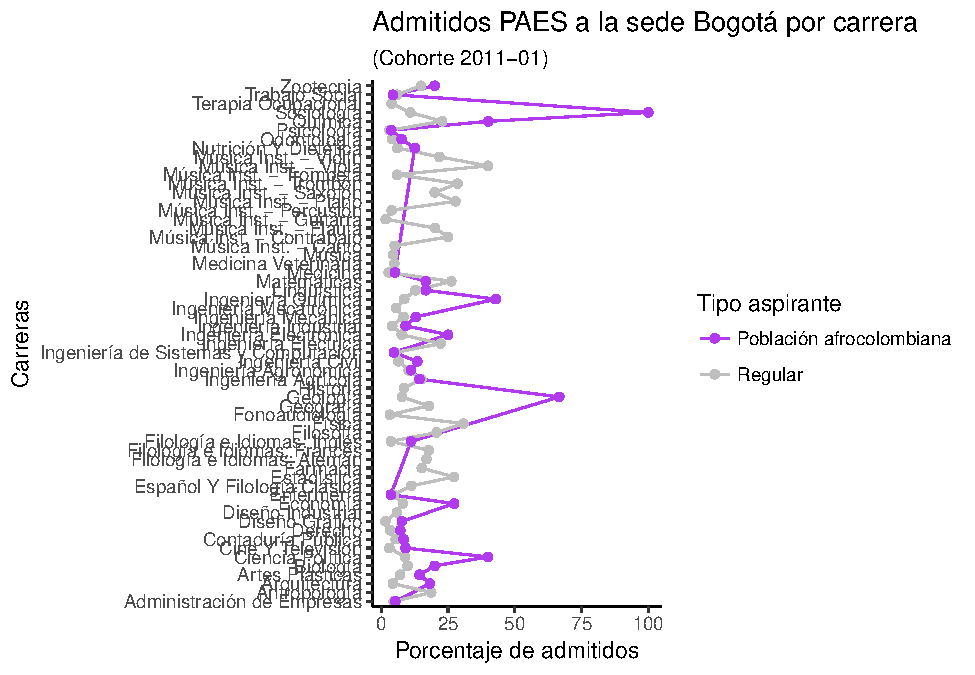
\includegraphics{bookdown_files/figure-latex/unnamed-chunk-11-4.pdf}

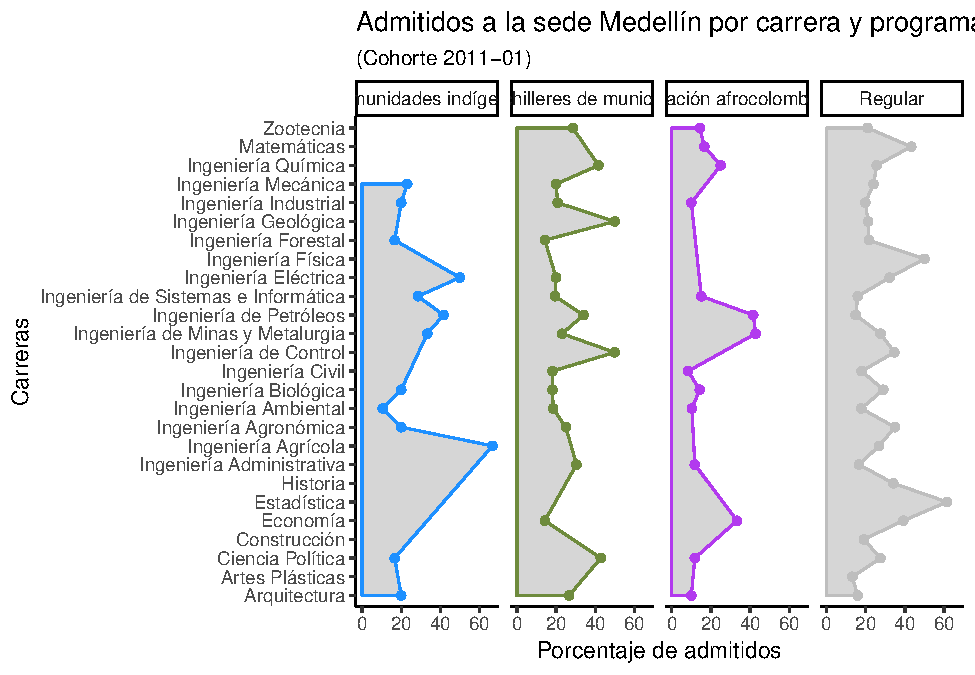
\includegraphics{bookdown_files/figure-latex/unnamed-chunk-12-1.pdf}
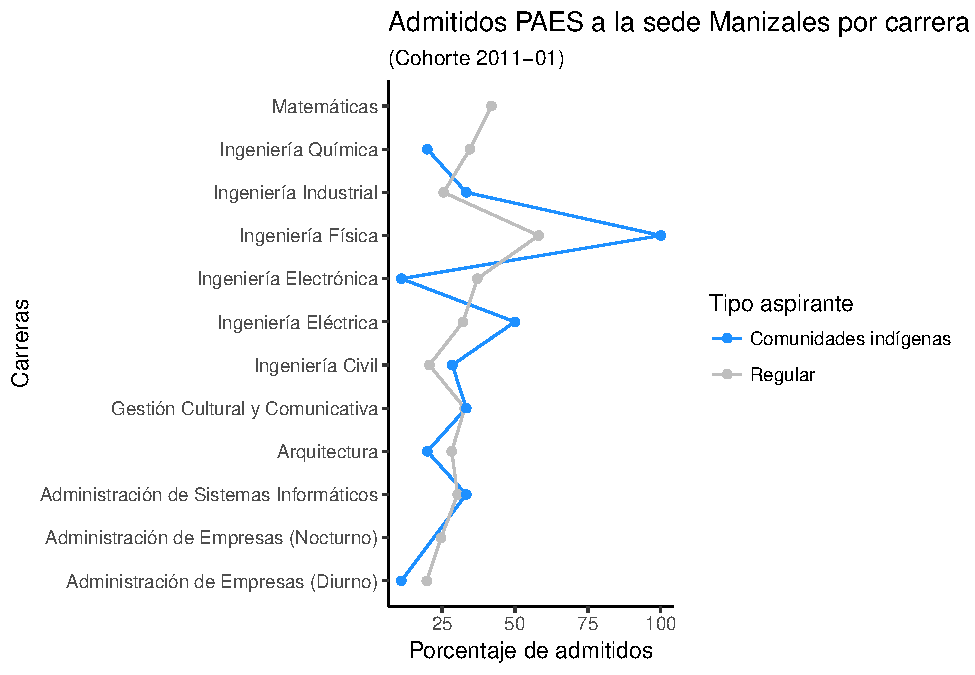
\includegraphics{bookdown_files/figure-latex/unnamed-chunk-12-2.pdf}
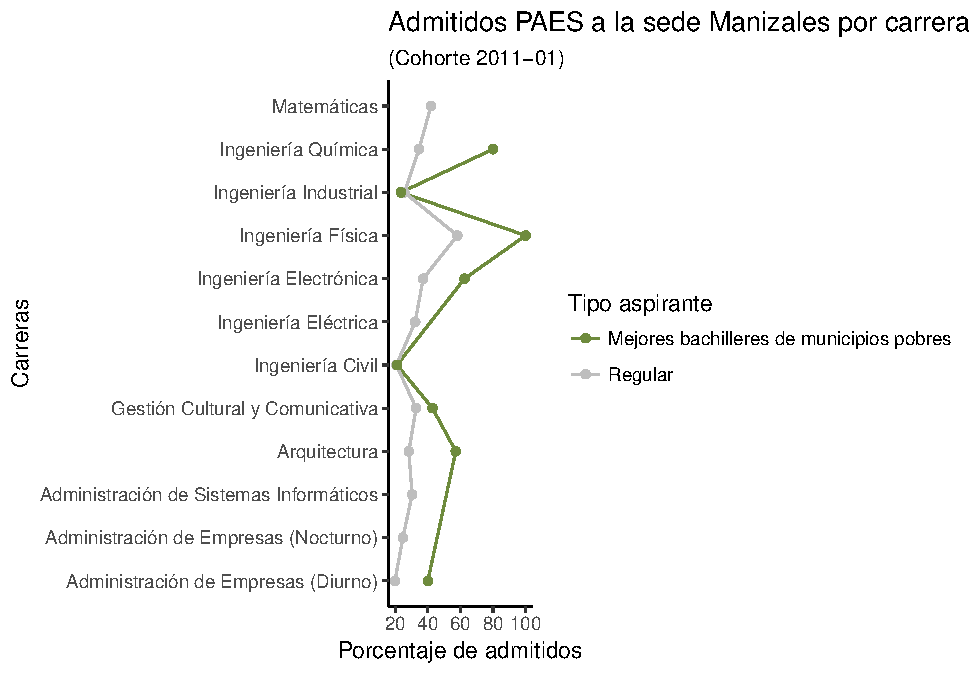
\includegraphics{bookdown_files/figure-latex/unnamed-chunk-12-3.pdf}
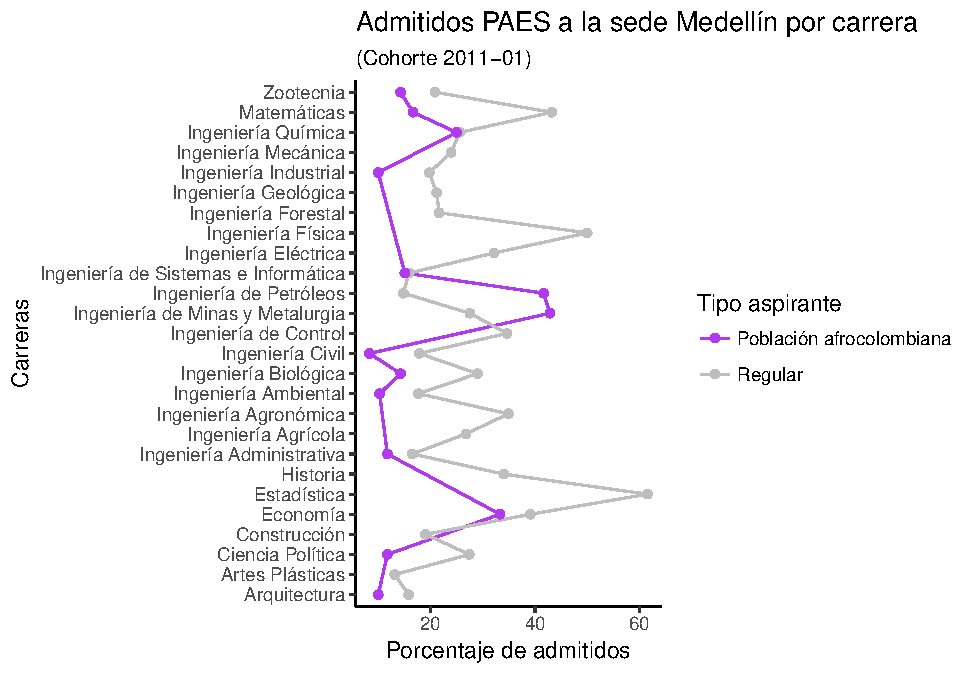
\includegraphics{bookdown_files/figure-latex/unnamed-chunk-12-4.pdf}

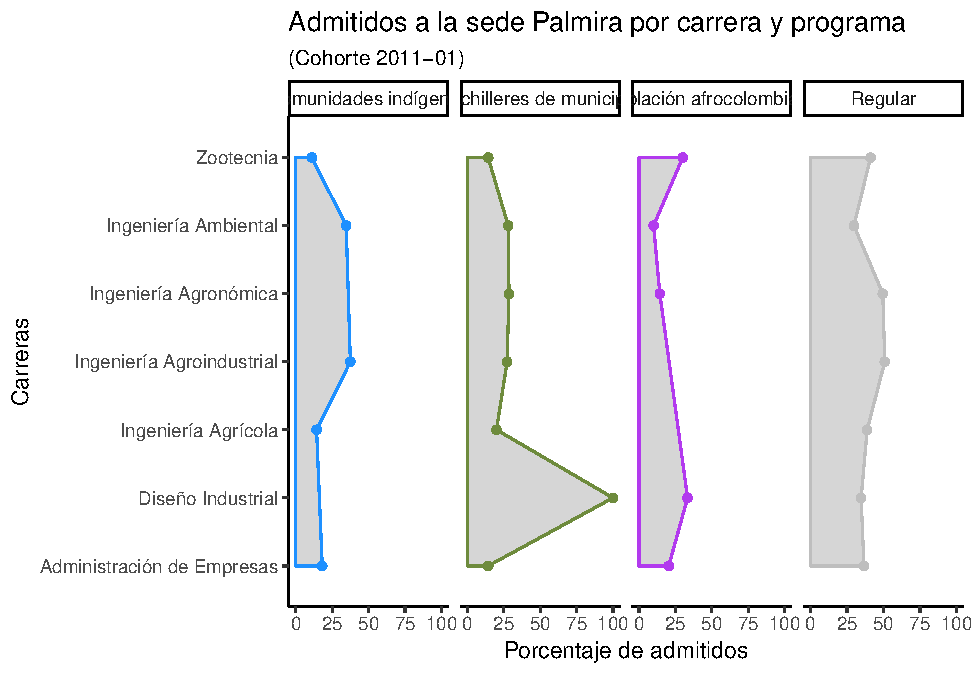
\includegraphics{bookdown_files/figure-latex/unnamed-chunk-13-1.pdf}
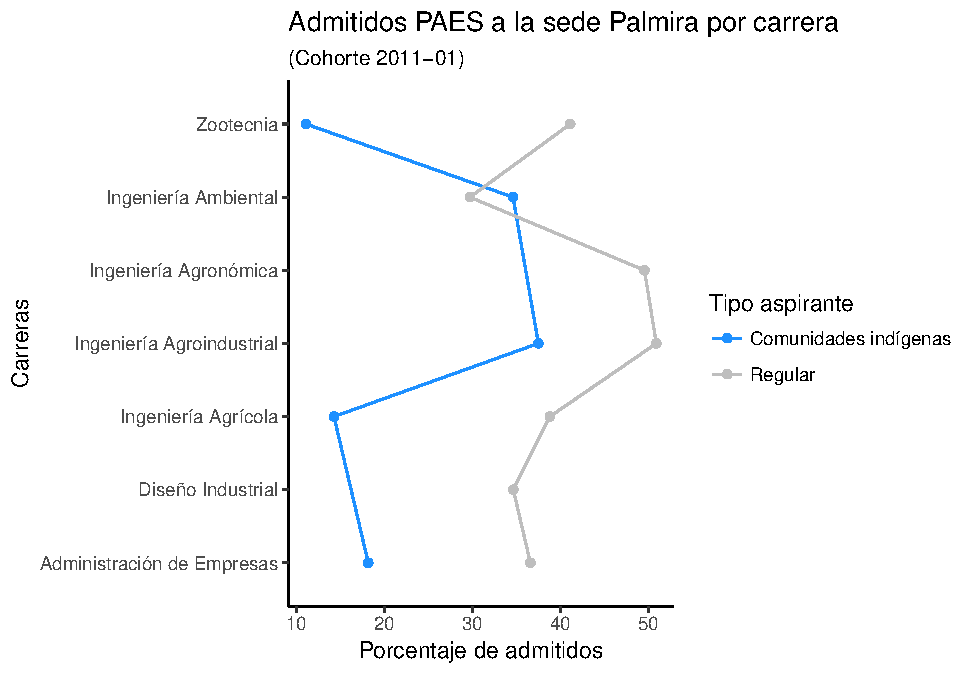
\includegraphics{bookdown_files/figure-latex/unnamed-chunk-13-2.pdf}
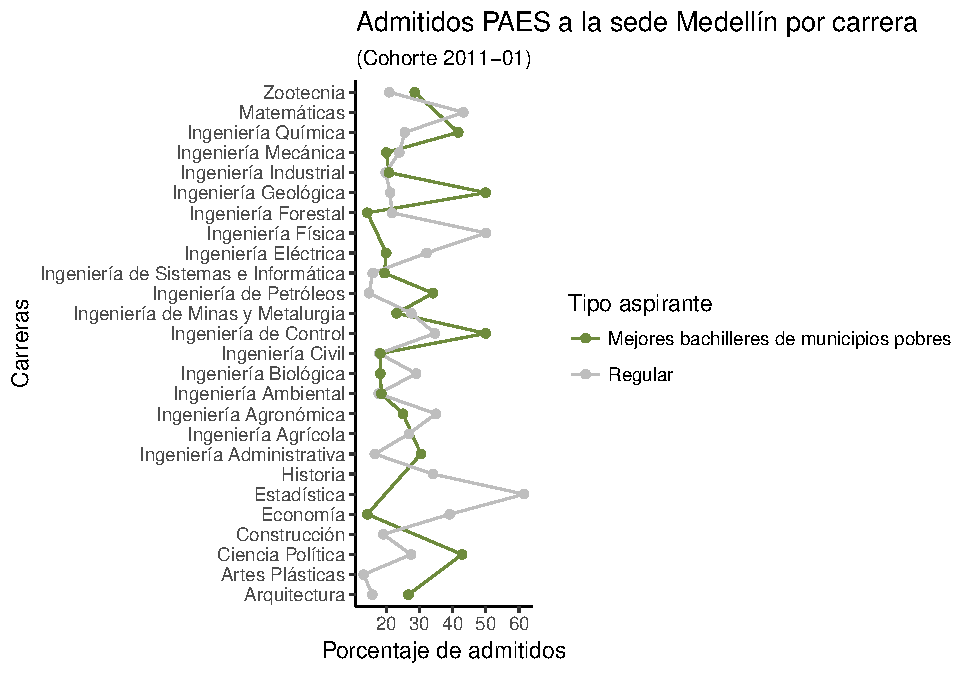
\includegraphics{bookdown_files/figure-latex/unnamed-chunk-13-3.pdf}
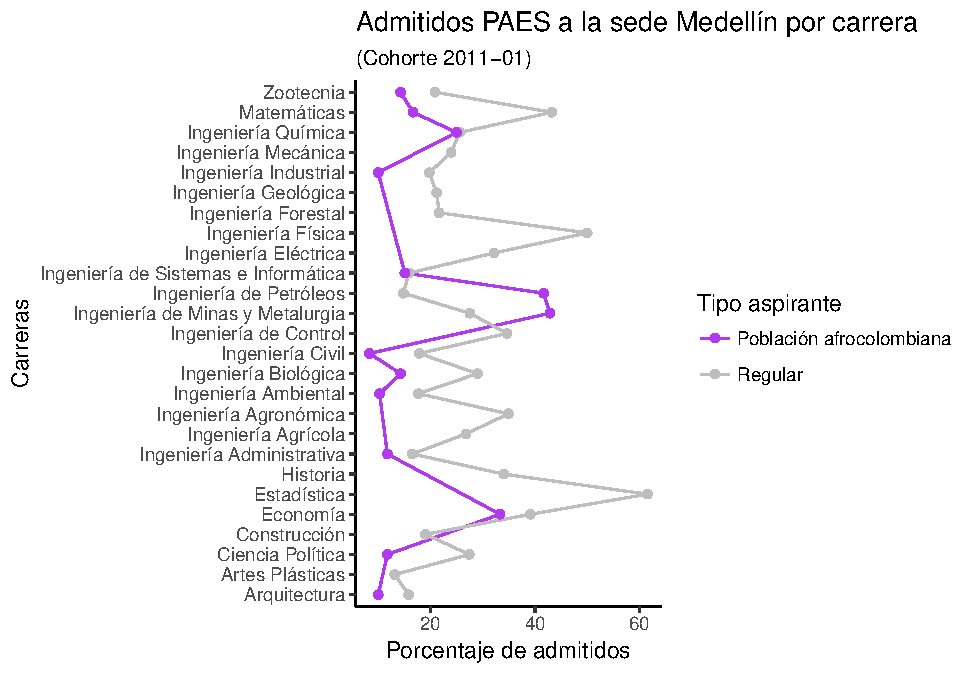
\includegraphics{bookdown_files/figure-latex/unnamed-chunk-13-4.pdf}

\subsection{Admitidos PAES por município de
residencia}\label{admitidos-paes-por-municipio-de-residencia}

\subsubsection{Todos los admitidos PAES}\label{todos-los-admitidos-paes}

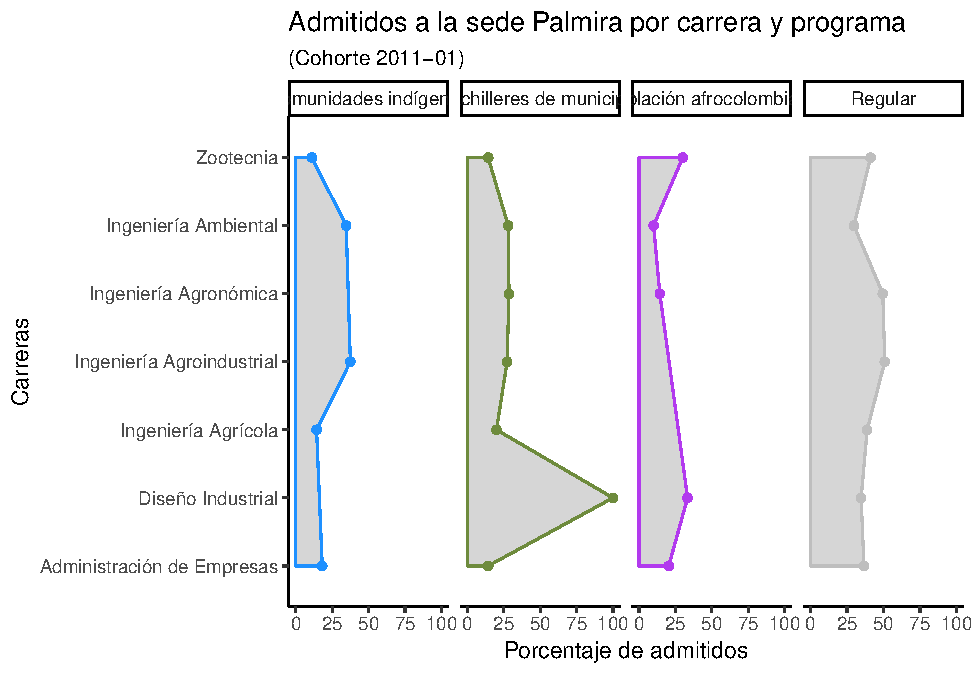
\includegraphics{bookdown_files/figure-latex/unnamed-chunk-14-1.pdf}

\includegraphics{bookdown_files/figure-latex/unnamed-chunk-14-2.pdf}

\subsubsection{Admitidos PAES de las comunidades
indígenas}\label{admitidos-paes-de-las-comunidades-indigenas}

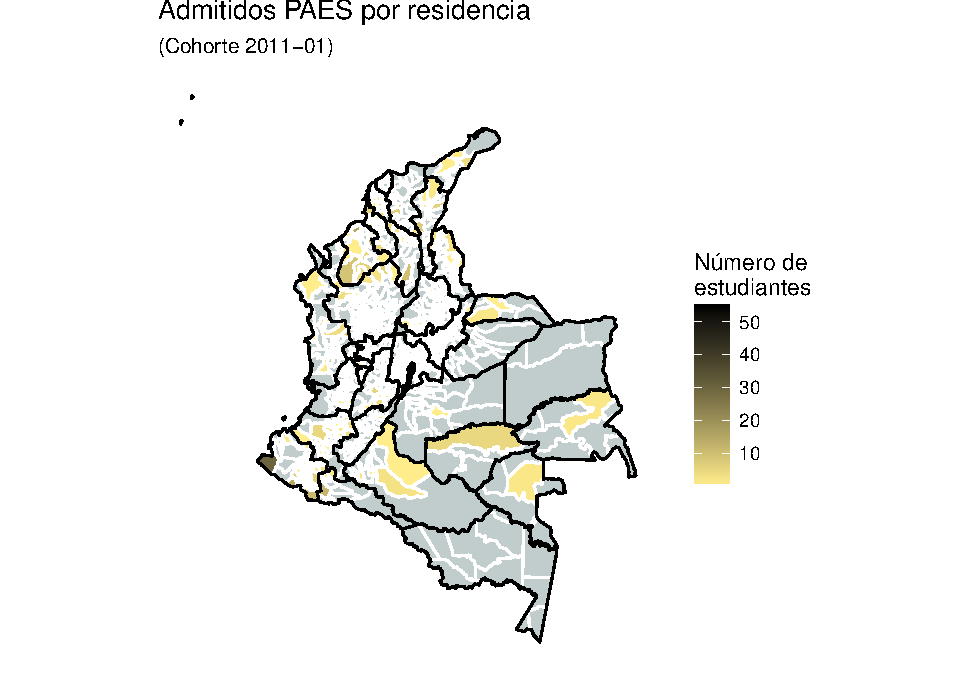
\includegraphics{bookdown_files/figure-latex/unnamed-chunk-15-1.pdf}

\subsubsection{Admitidos PAES de los mejores
bachilleres}\label{admitidos-paes-de-los-mejores-bachilleres}

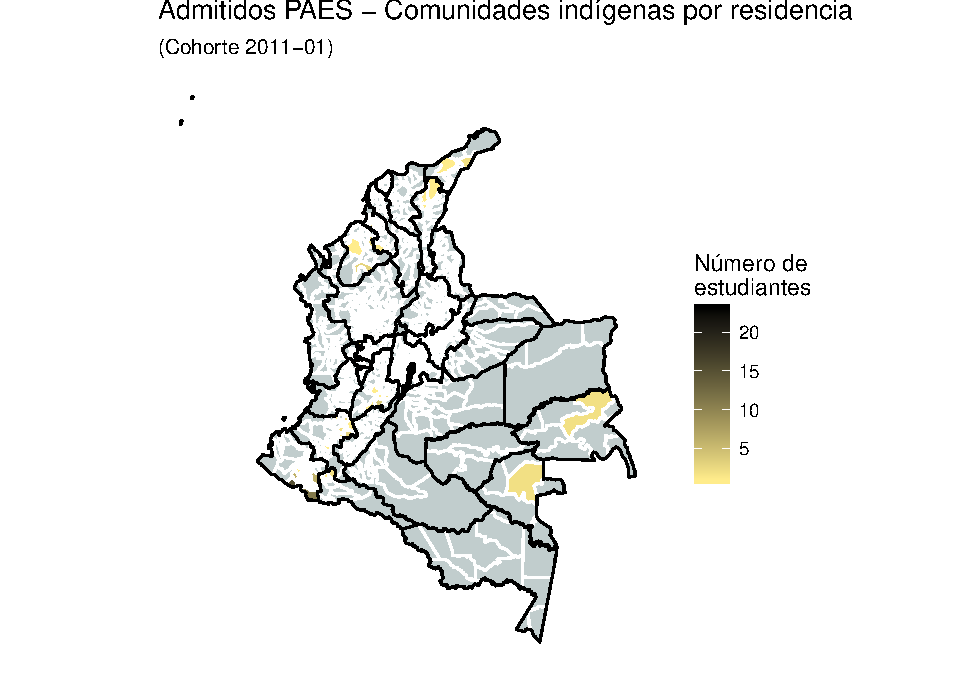
\includegraphics{bookdown_files/figure-latex/unnamed-chunk-16-1.pdf}

\subsubsection{Admitidos PAES de los mejores bachilleres de municipios
pobres}\label{admitidos-paes-de-los-mejores-bachilleres-de-municipios-pobres}

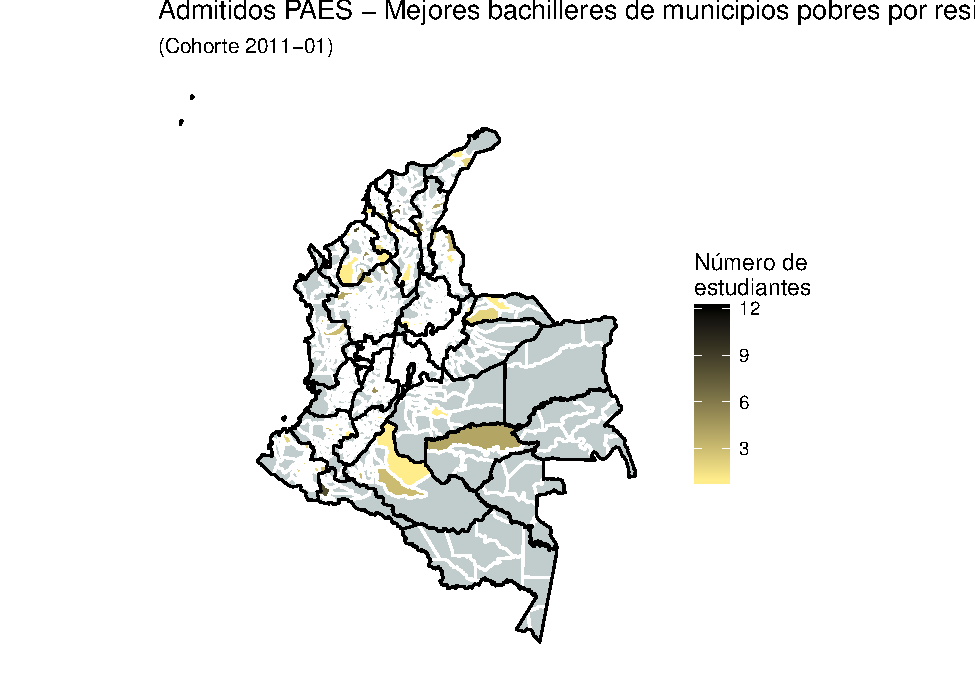
\includegraphics{bookdown_files/figure-latex/unnamed-chunk-17-1.pdf}

\subsubsection{Admitidos PAES de las poblaciones
afrocolombianas}\label{admitidos-paes-de-las-poblaciones-afrocolombianas}

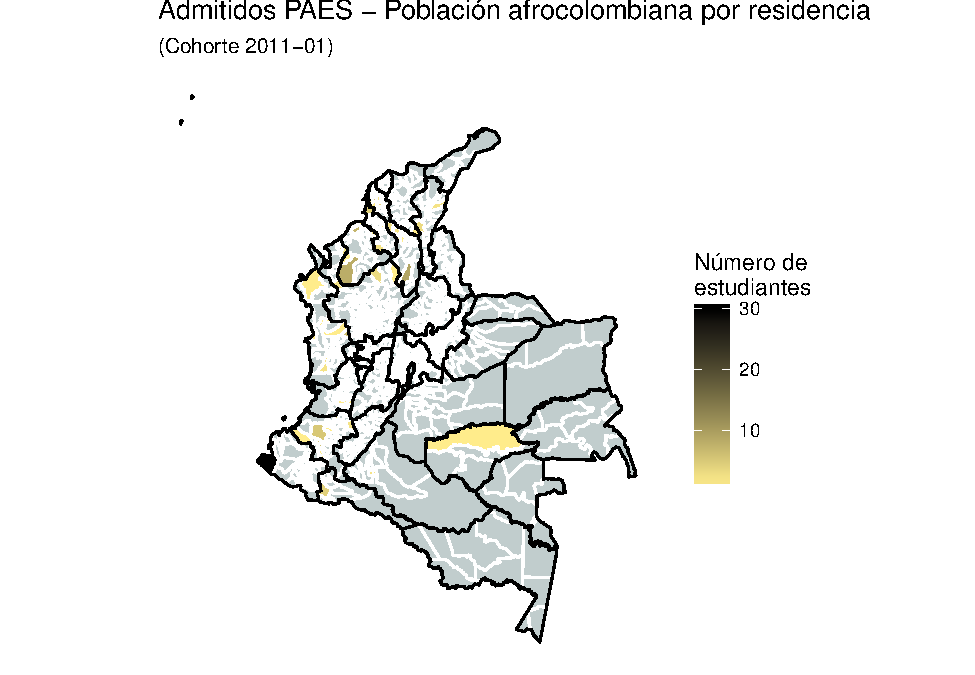
\includegraphics{bookdown_files/figure-latex/unnamed-chunk-18-1.pdf}

\subsection{Admitidos PAES por departamento de
residencia}\label{admitidos-paes-por-departamento-de-residencia}

\subsubsection{Todos los admitidos
PAES}\label{todos-los-admitidos-paes-1}

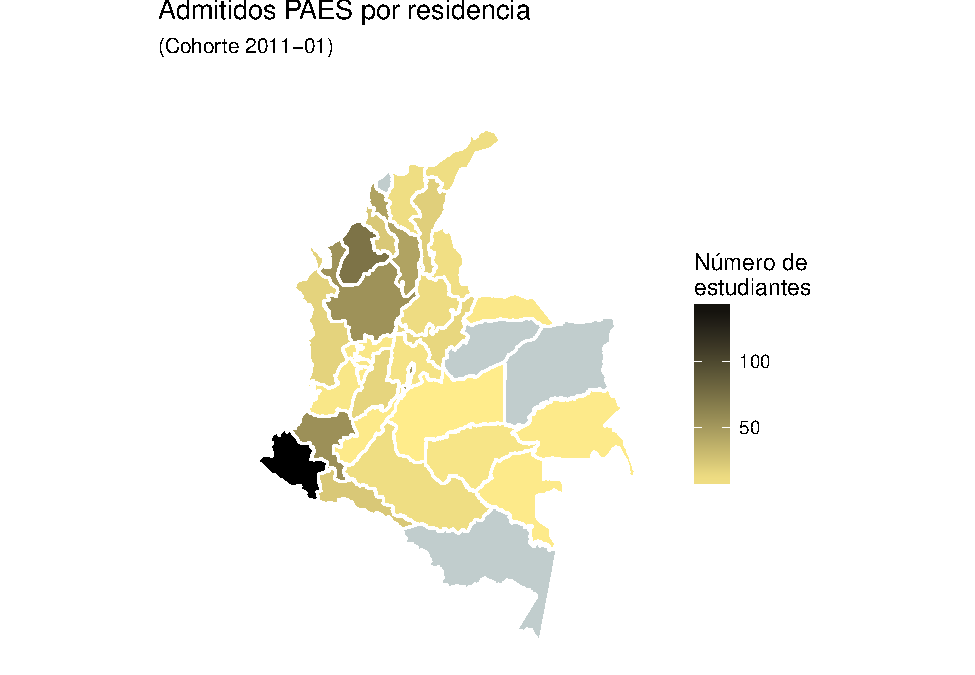
\includegraphics{bookdown_files/figure-latex/unnamed-chunk-19-1.pdf}

\includegraphics{bookdown_files/figure-latex/unnamed-chunk-19-2.pdf}

\subsubsection{Admitidos PAES de las comunidades
indígenas}\label{admitidos-paes-de-las-comunidades-indigenas-1}

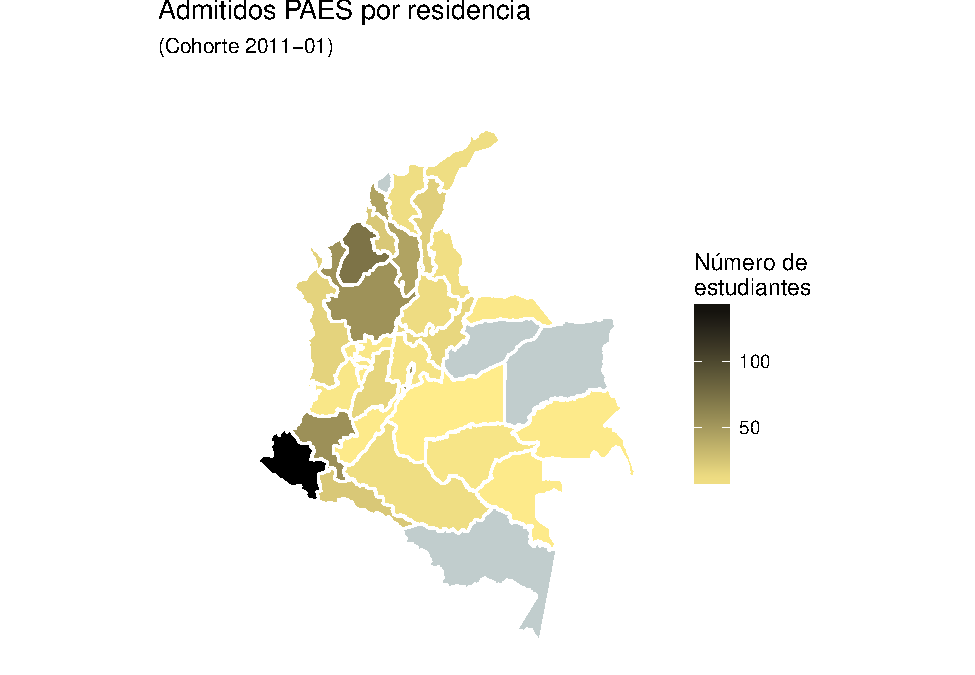
\includegraphics{bookdown_files/figure-latex/unnamed-chunk-20-1.pdf}

\subsubsection{Admitidos PAES de los mejores
bachilleres}\label{admitidos-paes-de-los-mejores-bachilleres-1}

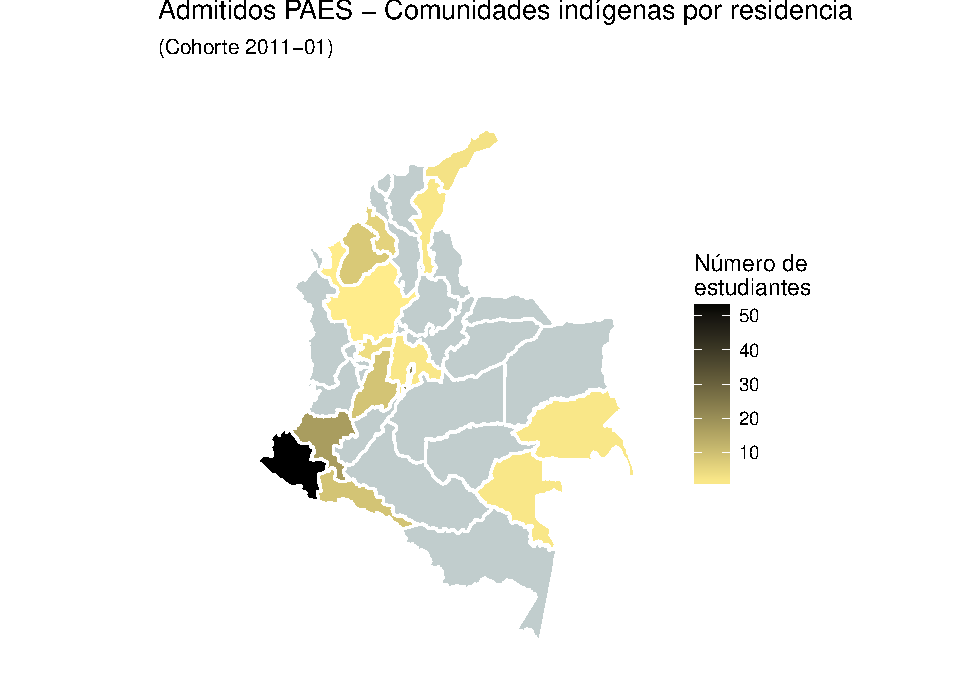
\includegraphics{bookdown_files/figure-latex/unnamed-chunk-21-1.pdf}

\subsubsection{Admitidos PAES de los mejores bachilleres de municipios
pobres}\label{admitidos-paes-de-los-mejores-bachilleres-de-municipios-pobres-1}

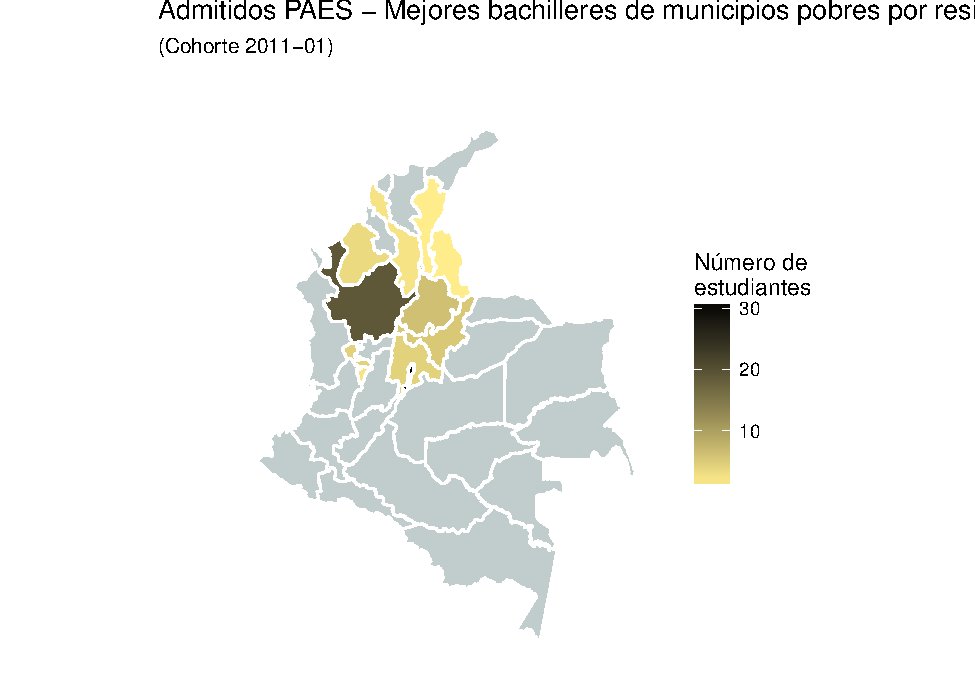
\includegraphics{bookdown_files/figure-latex/unnamed-chunk-22-1.pdf}

\subsubsection{Admitidos PAES de las poblaciones
afrocolombianas}\label{admitidos-paes-de-las-poblaciones-afrocolombianas-1}

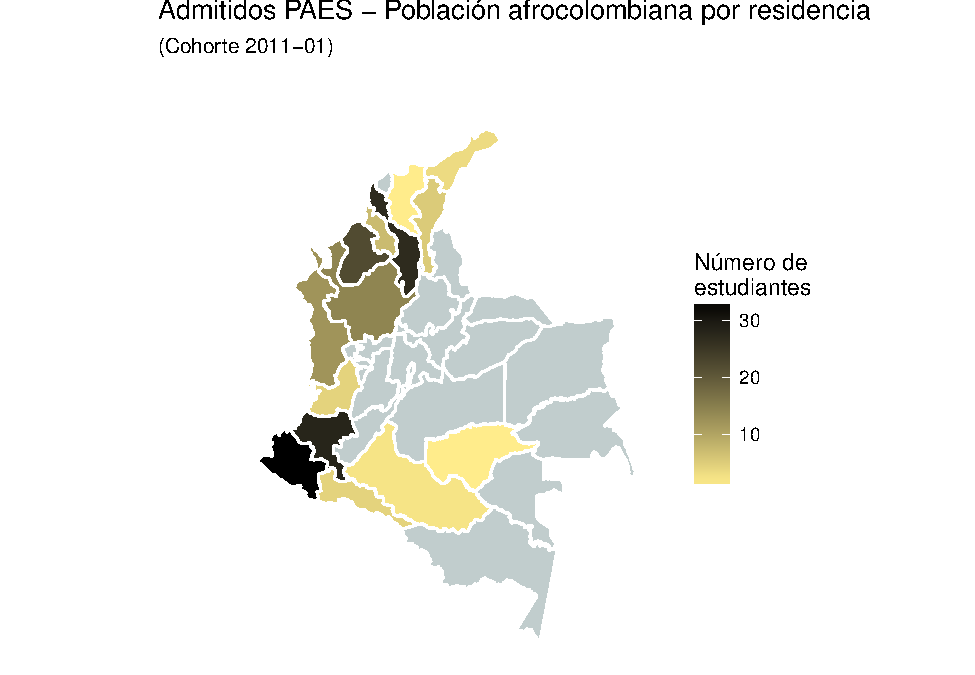
\includegraphics{bookdown_files/figure-latex/unnamed-chunk-23-1.pdf}

\section{Admisión PEAMA}\label{admision-peama}

En este capítulo se presenta una descripción del panorama general de
admisión de los estudiantes PEAMA de la cohorte 2011-01.

En primer lugar se observa cuales fueron los programas PEAMA por los que
los aspirantes fueron admitidos y que corresponden a la sede de
presencia nacional a la cual fueron admitidos:

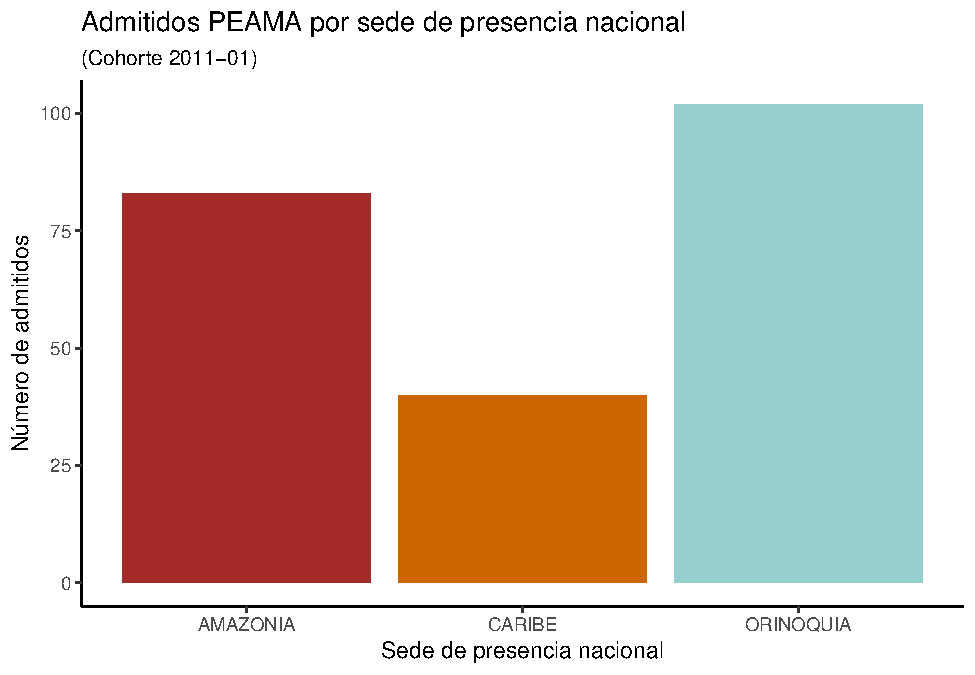
\includegraphics{bookdown_files/figure-latex/unnamed-chunk-25-1.pdf}

Observamos que la mayor parte entran por la \emph{Sede Orinoquia} con
102 admitidos, seguido por la \emph{Sede Amazonía} con 83 admitidos y en
tercer lugar la \emph{Sede Caribe} con 40 admitidos.

\subsection{Sexo de los admitidos}\label{sexo-de-los-admitidos-1}

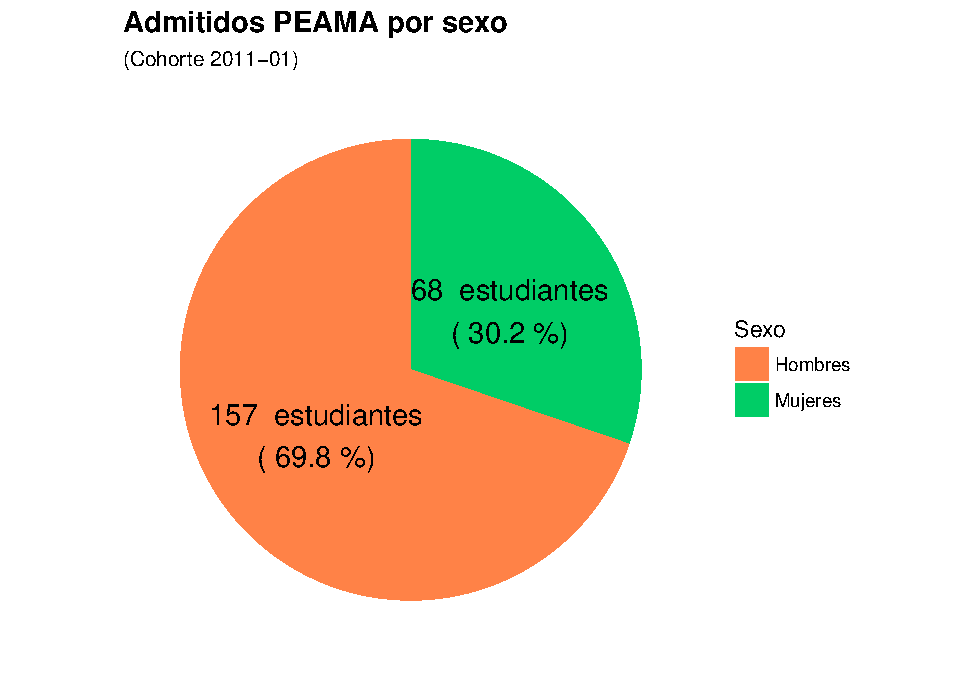
\includegraphics{bookdown_files/figure-latex/unnamed-chunk-26-1.pdf}
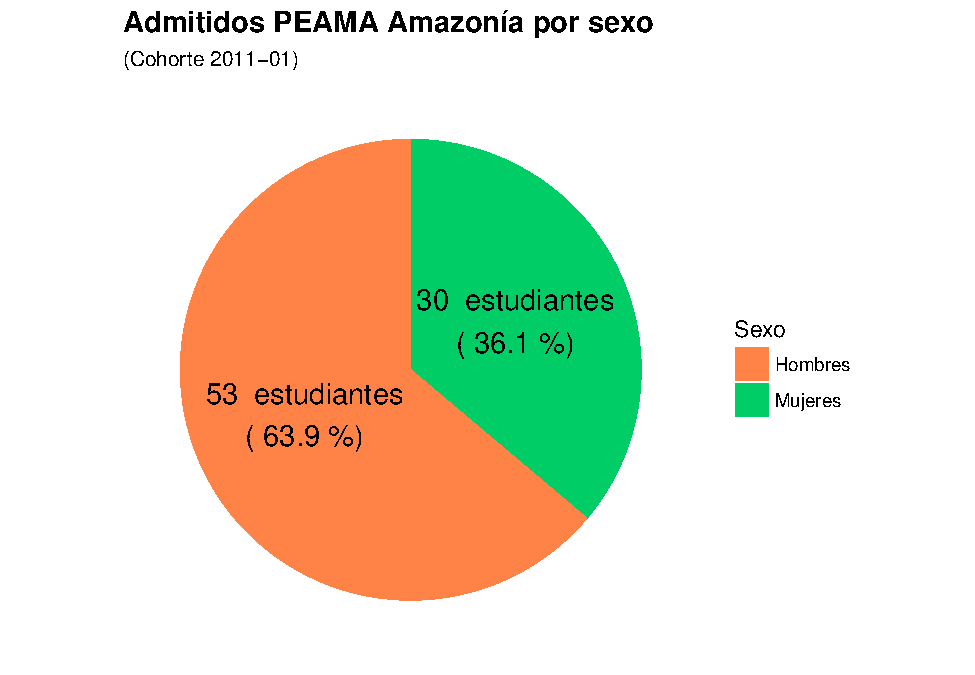
\includegraphics{bookdown_files/figure-latex/unnamed-chunk-26-2.pdf}
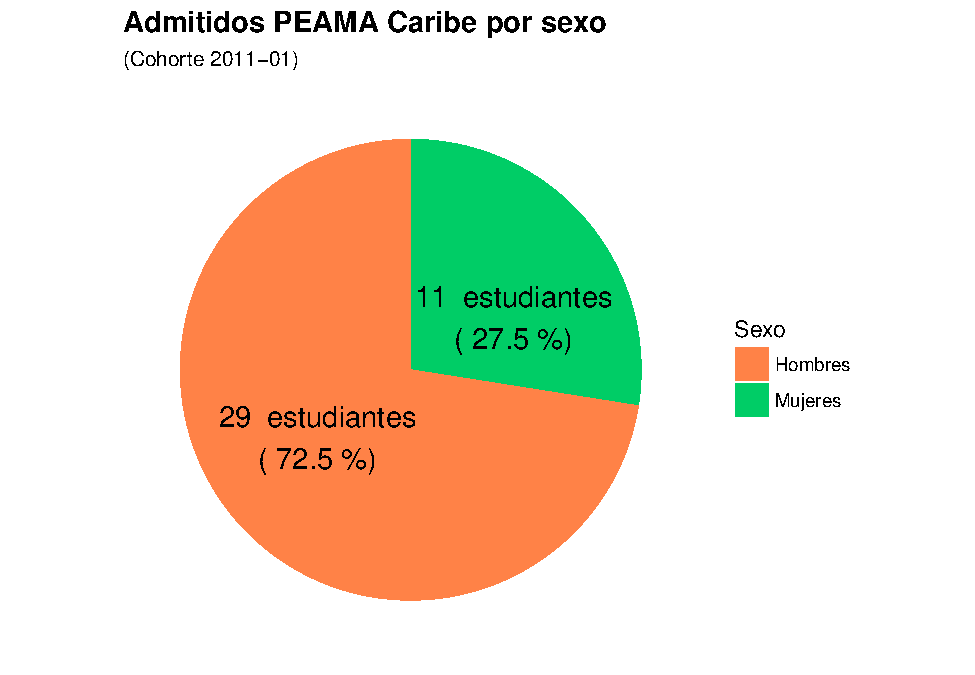
\includegraphics{bookdown_files/figure-latex/unnamed-chunk-26-3.pdf}
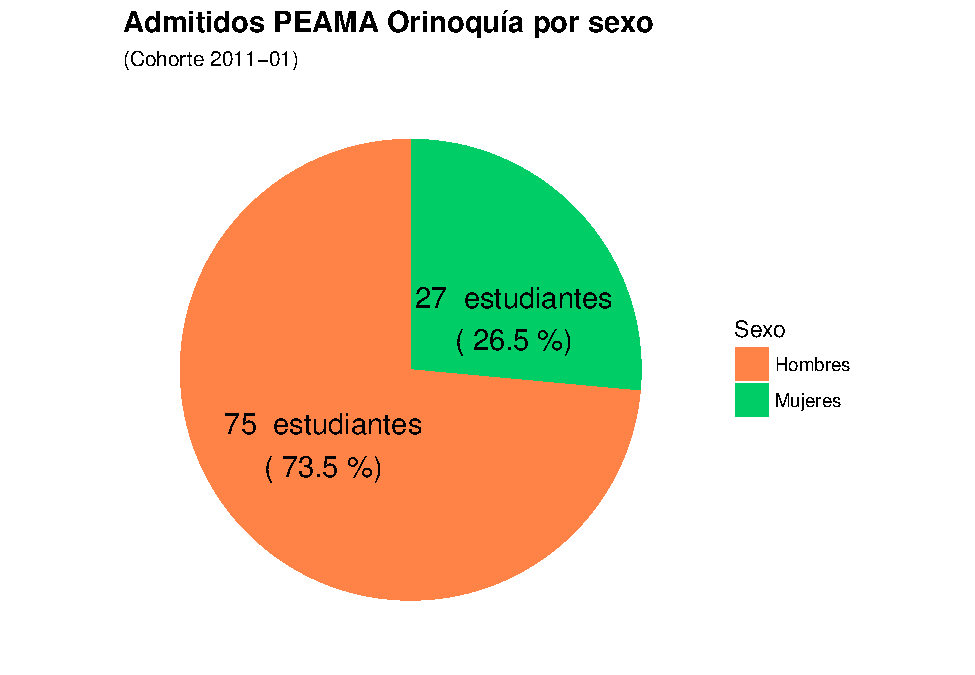
\includegraphics{bookdown_files/figure-latex/unnamed-chunk-26-4.pdf}

\subsection{Edad de los admitidos}\label{edad-de-los-admitidos-1}

\includegraphics{bookdown_files/figure-latex/unnamed-chunk-27-1.pdf}
\includegraphics{bookdown_files/figure-latex/unnamed-chunk-27-2.pdf}
\includegraphics{bookdown_files/figure-latex/unnamed-chunk-27-3.pdf}

\subsection{Sede andina de admisión}\label{sede-andina-de-admision}

\includegraphics{bookdown_files/figure-latex/unnamed-chunk-28-1.pdf}

\subsection{Sedes andinas de admisión y sede de presencia
nacional}\label{sedes-andinas-de-admision-y-sede-de-presencia-nacional}

\includegraphics{bookdown_files/figure-latex/unnamed-chunk-29-1.pdf}

\subsection{Programa de admisión}\label{programa-de-admision}

\includegraphics{bookdown_files/figure-latex/unnamed-chunk-30-1.pdf}

\subsection{Estrato de los admitidos}\label{estrato-de-los-admitidos}

\includegraphics{bookdown_files/figure-latex/unnamed-chunk-31-1.pdf}
\includegraphics{bookdown_files/figure-latex/unnamed-chunk-31-2.pdf}
\includegraphics{bookdown_files/figure-latex/unnamed-chunk-31-3.pdf}

\subsection{Puntaje total de admisión}\label{puntaje-total-de-admision}

\includegraphics{bookdown_files/figure-latex/unnamed-chunk-32-1.pdf}

\subsection{Admitidos PEAMA por
municipio}\label{admitidos-peama-por-municipio}

\subsubsection{Todos los admitidos
PEAMA}\label{todos-los-admitidos-peama}

\includegraphics{bookdown_files/figure-latex/unnamed-chunk-33-1.pdf}
\includegraphics{bookdown_files/figure-latex/unnamed-chunk-33-2.pdf}

\subsubsection{Admitidos PEAMA Amazonia}\label{admitidos-peama-amazonia}

\includegraphics{bookdown_files/figure-latex/unnamed-chunk-34-1.pdf}
\includegraphics{bookdown_files/figure-latex/unnamed-chunk-34-2.pdf}

\subsubsection{Admitidos PEAMA Caribe}\label{admitidos-peama-caribe}

\includegraphics{bookdown_files/figure-latex/unnamed-chunk-35-1.pdf}
\includegraphics{bookdown_files/figure-latex/unnamed-chunk-35-2.pdf}

\subsubsection{Admitidos PEAMA
Orinoquía}\label{admitidos-peama-orinoquia}

\includegraphics{bookdown_files/figure-latex/unnamed-chunk-36-1.pdf}
\includegraphics{bookdown_files/figure-latex/unnamed-chunk-36-2.pdf}

\subsection{Admitidos PEAMA por
departamento}\label{admitidos-peama-por-departamento}

\subsubsection{Todos los admitidos
PEAMA}\label{todos-los-admitidos-peama-1}

\includegraphics{bookdown_files/figure-latex/unnamed-chunk-37-1.pdf}
\includegraphics{bookdown_files/figure-latex/unnamed-chunk-37-2.pdf}

\subsubsection{Admitidos PEAMA
Amazonia}\label{admitidos-peama-amazonia-1}

\includegraphics{bookdown_files/figure-latex/unnamed-chunk-38-1.pdf}
\includegraphics{bookdown_files/figure-latex/unnamed-chunk-38-2.pdf}

\subsubsection{Admitidos PEAMA Caribe}\label{admitidos-peama-caribe-1}

\includegraphics{bookdown_files/figure-latex/unnamed-chunk-39-1.pdf}
\includegraphics{bookdown_files/figure-latex/unnamed-chunk-39-2.pdf}

\subsubsection{Admitidos PEAMA
Orinoquía}\label{admitidos-peama-orinoquia-1}

\includegraphics{bookdown_files/figure-latex/unnamed-chunk-40-1.pdf}
\includegraphics{bookdown_files/figure-latex/unnamed-chunk-40-2.pdf}

\section{Normatividad}\label{normatividad}

Una de las mediciones fundamentales en la evaluación del impacto de los
programas PAES y PEAMA es hacer una validación de la normatividad
vigente y aplicable para la cohorte 2011-01, esto debido a que la
normatividad refleja que las zonas de impacto de los programas sean las
realmente escaladas, que se pertenezca a las poblaciones a quien va
realmente dirigida y que se les esten dando las oportunidades que estan
reglamentadas por ley y que aportan a la inclusión educativa en la
Universidad Nacional de Colombia:

\begin{table}

\caption{\label{tab:unnamed-chunk-42}Normatividad vigente y aplicable para la cohorte de estudio}
\centering
\begin{tabular}[t]{lrrlll}
\toprule
Tipo & N° & Fecha & Tema & Entidad Emisora o País & Interna o Externa\\
\midrule
Acuerdo & 22 & 1986 & Por el cual se dictan disposiciones acerca del ingreso a la Universidad de integrantes de comunidades indígenas. & Consejo Superior Universitario & Interna\\
Acuerdo & 93 & 1989 & Por el cual se crea el programa de admisión para mejores bachilleres de municipios pobres. & Consejo Superior Universitario & Interna\\
Acuerdo & 30 & 1990 & Por el cual se crea el programa de Mejores Bachilleres. & Consejo Superior Universitario & Interna\\
Acuerdo & 121 & 1991 & Por el cual se autoriza la reducción de la carga académica obligatoria a los estudiantes admitidos mediante los Acuerdos Nos. 22 de 1986 y 93 de 1989 o programas especiales. & Consejo Superior Universitario & Interna\\
Acuerdo & 3 & 1995 & Por el cual se establecen las políticas de Bienestar Universitario. & Consejo de Educación Superior (CESU) & Externa\\
\addlinespace
Acuerdo & 18 & 1999 & Por el cual se modifica el Acuerdo No. 22 de 1986, programa especial para la admisión Bachilleres miembros de Comunidades Indígenas. & Consejo Superior Universitario & Interna\\
Acuerdo & 25 & 2007 & Por se adopta el Programa Especial de Admisión y Movilidad Académica para las Sedes de Presencia Nacional. & Consejo Superior Universitario & Interna\\
Resolución & 1302 & 2007 & Por la cual se reglamenta el Programa Especial de Admisión y Movilidad Académica y se dictan algunas disposiciones para su implementación en la Sede Orinoquia de la Universidad Nacional de Colombia & Rectoria & Interna\\
Resolución & 16 & 2008 & Por lo cual se reglamenta el Programa Especial de Admisión y Movilidad Académica y se dictan algunas disposiciones para su implementación en la sede Caribe de la Universidad Nacional de Colombia & Rectoria & Interna\\
Resolución & 125 & 2008 & Por lo cual se reglamenta el Programa Especial de Admisión y Movilidad Académica y se dictan algunas disposiciones para su implementación en la sede Amazonia de la Universidad Nacional de Colombia & Rectoria & Interna\\
\addlinespace
Resolución & 1055 & 2008 & Por la cual se complementa la reglamentación del Programa Especial de Admisión y Movilidad Académica y se dictan algunas disposiciones para su implementación en las Sedes de Presencia Nacional de la Universidad Nacional de Colombia & Rectoria & Interna\\
Resolución & 1708 & 2009 & Por la cual se establecen disposiciones para ampliar en la Sede Amazonía la oferta de programas curriculares del Programa Especial de Admisión y Movilidad Académica PEAMA al área de ciencias sociales e incluir nuevos programas de las áreas de ciencias agropecuarias e ingeniería & Rectoria & Interna\\
Acuerdo & 13 & 2009 & Por el cual se crea el programa de admisión especial a mejores bachilleres de población negra, afrocolombiana, palenquera y raizal. & Consejo Superior Universitario & Interna\\
Acuerdo & 7 & 2010 & Por el cual se determina y organiza el Sistema de Bienestar Universitario en la Universidad Nacional de Colombia. & Consejo Superior Universitario & Interna\\
Acuerdo & 28 & 2010 & Por el cual se reglamenta el Sistema de Acompañamiento Estudiantil en la Universidad Nacional de Colombia. & Consejo Académico & Interna\\
\addlinespace
Acuerdo & 201 & 2015 & Por el cual se adopta el Programa Especial de Admisión y Movilidad Académica - PEAMA para las Sedes de Bogotá, Manizales, Medellín y Palmira de la Universidad Nacional de Colombia. & Consejo Superior Universitario & Interna\\
Acuerdo & 215 & 2015 & Por el cual se crea el programa de admisión especial para bachilleres víctimas del conflicto armado interno en Colombia. & Consejo Superior Universitario & Interna\\
Resolución & 55 & 2016 & Por la cual se reglamenta para el Programa Especial de Admisión y Movilidad Académica (PEAMA) de Presencia Nacional, la admisión, la matrícula inicial para admitidos, la región de influencia para las Sedes Amazonia, Caribe, Orinoquia y Tumaco y los estímulos económicos para el personal académico de la Universidad Nacional de Colombia y se deroga la Resolución 887 de 2015 de la Rectoría. & Rectoría & Interna\\
Resolución & 654 & 2016 & Por la cual se modifican los artículos 4 y 5 de la Resolución 55 de 2016 de la Rectoría que reglamentó para el Programa Especial de Admisión y Movilidad Académica (PEAMA) para las Sedes de Presencia Nacional, la admisión, la matrícula inicial para admitidos, la región de influencia para las Sedes Amazonia, Caribe, Orinoquia y Tumaco y los estímulos económicos para el personal académico de la Universidad Nacional de Colombia. & Rectoría & Interna\\
Resolución & 658 & 2016 & Por la cual se reglamenta para el Programa Especial de Admisión y Movilidad Académica (PEAMA) de la Sede Manizales- PEAMA CALDAS, la admisión, la matrícula inicial para admitidos, la región de influencia para la Sede Manizales y los estímulos económicos para el personal académico de la Universidad Nacional de Colombia. & Rectoría & Interna\\
Resolución & 108 & 2017 & Por la cual se modifica el artículo 4 de la Resolución 55 de 2016 de la Rectoría y se deroga el artículo 1 de la Resolución 654 de 2016 de la Rectoría. & Rectoría & Interna\\
\bottomrule
\end{tabular}
\end{table}

\subsection{Validación de la normatividad vigente y aplicable a los
PAES}\label{validacion-de-la-normatividad-vigente-y-aplicable-a-los-paes}

\subsubsection{Puntaje en examen de
admisión}\label{puntaje-en-examen-de-admision-1}

Como dice el \textbf{acuerdo 22 de 1986 del CSU en el articulo dos} y el
\textbf{acuerdo 18 de 1999 del CSU en el articulo dos} para las
\emph{comunidades indigenas} y el \textbf{acuerdo 93 de 1989 del CSU en
el articulo dos} para los \emph{mejores bachilleres de municipios
pobres}, los estudiantes admitidos por estas dos modalidades deben tener
un puntaje de admisión mayor o igual al último admitido de manera
regular, además como dice el\textbf{acuerdo 30 de 1990 del CSU en el
articulo dos} para los \emph{mejores bacilleres} y el \textbf{acuerdo 13
de 2009 del CSU en el articulo dos} para las \emph{poblaciones
afrocolombianas} son admitidos en los mismos términos que los
estudiantes de admisión regular, luego para ellos también aplica tener
el puntaje de admisión es mayor o igual al último admitido de manera
regular.

Se observa, como una línea roja, el menor puntaje (451.2525) obtenido
por los admitidos de manera regular y es claro que en todos los
programas PAES se satisface la norma del menor puntaje de admisión
posible para ellos.

\includegraphics{bookdown_files/figure-latex/unnamed-chunk-43-1.pdf}

\subsubsection{Razón de admitidos PAES por programa vs.~la cantidad de
cupos ofertados por el programa
curricular}\label{razon-de-admitidos-paes-por-programa-vs.la-cantidad-de-cupos-ofertados-por-el-programa-curricular}

Como dice el \textbf{acuerdo 22 de 1986 del CSU en el articulo uno} para
las \emph{comunidades indigenas} y el \textbf{acuerdo 93 de 1989 del CSU
en el articulo uno} para los \emph{mejores bachilleres de municipios
pobres} y el \textbf{acuerdo 13 de 2009 del CSU en el articulo tres}
para las \emph{poblaciones afrocolombianas} los cuales establecen que se
deben destinar por lo menos el \(2\%\) de los cupos por carrera a cada
uno de los tres programas PAES anteriormente mencionados.

Con el objetivo de validar las normas anteriormente mencionadas se
observa a continuación una comparación del número de admitidos de cada
uno de los programas PAES por carrera contra la cantidad de cupos.

Primero para el caso de la sede Bogotá se tiene que la razón de
admitidos PAES comparada con el número de cupos ofertados por programa
curricular es en todos los casos igual o superior al 2\%. En los casos
de la sede Medellín y la sede Manizales se observa que en la mayoría de
los casos la razón de admitidos PAES por programa curricular contra la
cantidad de cupos disponibles está en 2\% o es superior, en unos pocos
casos es inferior al 2\% pero recordemos que la norma es sensible a un
redondeo de la cantidad de cupos que les corresponden a los programas,
también se puede dar el caso en que la demanda de un programa es
inferior la cantidad de cupos reservados a los PAES. Por otra parte,
para la sede Palmira, todos los programas tienen una razón superior al
2\%.

\includegraphics{bookdown_files/figure-latex/unnamed-chunk-45-1.pdf}

\includegraphics{bookdown_files/figure-latex/unnamed-chunk-46-1.pdf}

\includegraphics{bookdown_files/figure-latex/unnamed-chunk-47-1.pdf}

\includegraphics{bookdown_files/figure-latex/unnamed-chunk-48-1.pdf}

\subsubsection{Estrato socio-económico de los PAES de poblaciones
afrocolombianas}\label{estrato-socio-economico-de-los-paes-de-poblaciones-afrocolombianas}

El \textbf{acuerdo 13 de 2009 del CSU en el articulo uno} para las
\emph{poblaciones afrocolombianas} establece que los admitidos por esta
modalidad deberan pertenecer a los estratos 1 ó 2. Se observa a
continuacíon que, aunque la mayoría de los admitidos cumple con la
normatividad, existen unos cuantos que o bien pertenecen al estrato 3 o
bien se rotulan como estrato 0. Lo cual es claramente una falta de
cumplimiento en a norma:

\includegraphics{bookdown_files/figure-latex/unnamed-chunk-49-1.pdf}
\includegraphics{bookdown_files/figure-latex/unnamed-chunk-49-2.pdf}

\subsection{Validación de la normatividad vigente y aplicable a los
PEAMA}\label{validacion-de-la-normatividad-vigente-y-aplicable-a-los-peama}

\subsubsection{Puntaje total de
admisión}\label{puntaje-total-de-admision-1}

Como dice la \textbf{resolución 125 de 2008 de la Rectoría en el
artículo cuatro} y la \textbf{resolución 1708 de 2009 de la Rectoría en
el artículo dos} para el programa \emph{PEAMA Amazonía}, la
\textbf{resolución 16 de 2008 de la rectoría en el artículo tres} para
el programa \emph{PEAMA Caribe} y la \textbf{resolución 1302 de 2007 de
la rectoría en el artículo cuatro} para el programa \emph{PEAMA
Orinoquía}, los estudiantes admitidos por estas modalidades deben tener
un puntaje de admisión mayor o igual al último admitido de manera
regular.

\includegraphics{bookdown_files/figure-latex/unnamed-chunk-50-1.pdf}

\subsubsection{Departamento de residencia de los
admitidos}\label{departamento-de-residencia-de-los-admitidos}

Como dice el \textbf{acuerdo 25 de 2007 del CSU en el artículo dos} los
estudiantes que se presentan a través de la admisión en las sedes de
presencia nacional deben tener domicilio en la región de alcance de la
misma. la \textbf{resolución 125 de 2008 de la Rectoría en el artículo
dos} establece para el programa \emph{PEAMA Amazonía} como zona de
residencia los departamentos de Amazonía, Guainia, Putumayo o Vaupés, la
\textbf{resolución 16 de 2008 de la rectoría en el artículo dos}
establece para el programa \emph{PEAMA Caribe} que los aspirantes deben
residir en el archipielago de San Andrés (mediante certificación de la
OCCRE) y la \textbf{resolución 1302 de 2007 de la rectoría en el
artículo dos} establece para el programa \emph{PEAMA Orinoquía} como
zona de residencia los departamentos de Arauca, Casanare, Guainia,
Guaviare y Vichada.

\includegraphics{bookdown_files/figure-latex/unnamed-chunk-51-1.pdf}

Observamos que los admitidos a través del programa \emph{PEAMA Amazonía}
provienen de los departamentos: Amazonía, Putumayo, Caquetá y Bogotá
D.C., de donde se encuentra que los dos últimos departamentos se salen
de la norma anteriormente descrita.

\includegraphics{bookdown_files/figure-latex/unnamed-chunk-52-1.pdf}

Para el caso del programa \emph{PEAMA Caribe} se encuentra que la
residencia de los admitidos es de los departamentos: Archipielago de San
Andrés, Providencia y Santa Catalina, Magdalena y Cesar, nuevamente
estos dos últimos no concuerdan con la norma correspondiente.

\includegraphics{bookdown_files/figure-latex/unnamed-chunk-53-1.pdf}

Finalmente en el programa \emph{PEAMA Orinoquía} se encuentran que son
residentes de los departamentos: Aráuca, Casanare, Guainia, Guaviare,
Meta y Vichada. El departamento del Meta no se encuentra completado en
la norma aplicable.

\subsubsection{Cupos por programa}\label{cupos-por-programa}

Como se dispone en la \textbf{resolución 125 de 2008 de la Rectoría en
el artículo tres} y ampliado en la \textbf{resolución 1708 de 2009 de la
Rectoría en el artículo uno} para el programa \emph{PEAMA Amazonía}, la
\textbf{resolución 16 de 2008 de la rectoría en el artículo tres} para
el programa \emph{PEAMA Caribe} y la \textbf{resolución 1302 de 2007 de
la rectoría en el artículo cuatro} para el programa \emph{PEAMA
Orinoquía}, los estudiantes admitidos por estas modalidades pueden tomar
los cupos de admisión para las carreras establecidos en la norma y la
cantidad de cupos tambien dispuestos ahí mismo. Se observa en color azúl
los cupos por carrera dictados por la norma y en rojo los admitidos a
los mismos.

\includegraphics{bookdown_files/figure-latex/unnamed-chunk-54-1.pdf}
\includegraphics{bookdown_files/figure-latex/unnamed-chunk-54-2.pdf}
\includegraphics{bookdown_files/figure-latex/unnamed-chunk-54-3.pdf}
\includegraphics{bookdown_files/figure-latex/unnamed-chunk-54-4.pdf}

Se observa que la norma sólo está siendo violada por seis admitidos del
\emph{PEAMA AMAZONÍA} a carreras de Medellín que no se encontraban
aprobadas por las normas, específicamente dos a Ingeniería
Administrativa, uno a Ingeniería de Minas y Metalurgia, dos a Ingeniería
de Petroleos y uno a Zootecnia.

\subsubsection{Total de cupos}\label{total-de-cupos}

De acuerdo al \textbf{acuerdo 25 de 2007 del CSU en el considerando
cuatro} se espera la universidad otorgue el \(1\%\) de cupos a
bachilleres de los departamentos en los que no haya instituciones de
educación superior y otro \(1\%\) a los aspirantes que provengan de
municipios de difícil acceso o con problemas de orden público, dando así
una norma de \(2\%\) de cupos que deben ser otorgados por un sistema
especial de admisión en la Universidad. El programa PEAMA, de acuerdo a
las normas \textbf{resolución 125 de 2008 de la Rectoría en el artículo
tres} y ampliado en la \textbf{resolución 1708 de 2009 de la Rectoría en
el artículo uno} para el programa \emph{PEAMA Amazonía}, la
\textbf{resolución 16 de 2008 de la rectoría en el artículo tres} para
el programa \emph{PEAMA Caribe} y la \textbf{resolución 1302 de 2007 de
la rectoría en el artículo cuatro} para el programa \emph{PEAMA
Orinoquía}, establece un total de 190 cupos para estos programas, dado
que para a cohorte de estudio el número total de cupos disponibles para
admisión es del 5083 cupos según la \textbf{resolución que la DNA nos
debería indicar}. De donde el porcentaje de cupos de admisión otorgados
por esta modalidad especial es del \(3.8\%\), dando así un cumplimiento
satisfactorio de la norma.

\section{Impácto de los programas especiales de admisión PAES y
PEAMA}\label{impacto-de-los-programas-especiales-de-admision-paes-y-peama}

\subsection{Porcentajes de admisión}\label{porcentajes-de-admision}

\includegraphics{bookdown_files/figure-latex/unnamed-chunk-56-1.pdf}

\subsubsection{Índice de absorción del admitido
Regular}\label{indice-de-absorcion-del-admitido-regular}

\begin{table}

\caption{\label{tab:unnamed-chunk-57}Índice de absorción para los admitidos regulares}
\centering
\begin{tabular}[t]{rrr}
\toprule
ASPIRANTES & ADMITIDOS & INDICE\\
\midrule
64659 & 5872 & 9.08\\
\bottomrule
\end{tabular}
\end{table}

\subsubsection{Índices de absorción del admitido
PAES}\label{indices-de-absorcion-del-admitido-paes}

\begin{table}

\caption{\label{tab:unnamed-chunk-58}Índices de absorción por tipo de PAES}
\centering
\begin{tabular}[t]{lrrr}
\toprule
PAES & ASPIRANTES & ADMITIDOS & INDICE\\
\midrule
Comunidades indígenas & 1091 & 141 & 12.92\\
Mejores bachilleres & 189 & 78 & 41.27\\
Mejores bachilleres de municipios pobres & 1680 & 224 & 13.33\\
Población afrocolombiana & 1472 & 163 & 11.07\\
\bottomrule
\end{tabular}
\end{table}

\subsubsection{Índices de absorción del admitido
PEAMA}\label{indices-de-absorcion-del-admitido-peama}

\begin{table}

\caption{\label{tab:unnamed-chunk-59}Índices de absorción por tipo de PEAMA}
\centering
\begin{tabular}[t]{lrrr}
\toprule
PEAMA & ASPIRANTES & ADMITIDOS & INDICE\\
\midrule
PEAMA - Amazonía & 403 & 83 & 20.60\\
PEAMA - Caribe & 266 & 40 & 15.04\\
PEAMA - Orinoquía & 871 & 102 & 11.71\\
\bottomrule
\end{tabular}
\end{table}

\subsection{Puntaje de admisión}\label{puntaje-de-admision}

\includegraphics{bookdown_files/figure-latex/unnamed-chunk-60-1.pdf}

\subsection{Ubicación de los
admitidos}\label{ubicacion-de-los-admitidos}

\subsubsection{Departamentos}\label{departamentos}

Todos los admitidos PAES

\includegraphics{bookdown_files/figure-latex/unnamed-chunk-62-1.pdf}
\includegraphics{bookdown_files/figure-latex/unnamed-chunk-62-2.pdf}

Todos los admitidos PEAMA

\includegraphics{bookdown_files/figure-latex/unnamed-chunk-63-1.pdf}
\includegraphics{bookdown_files/figure-latex/unnamed-chunk-63-2.pdf}

Todos los admitidos REGULARES

\includegraphics{bookdown_files/figure-latex/unnamed-chunk-64-1.pdf}
\includegraphics{bookdown_files/figure-latex/unnamed-chunk-64-2.pdf}

\subsubsection{Municipios}\label{municipios}

Todos los admitidos PAES

\includegraphics{bookdown_files/figure-latex/unnamed-chunk-65-1.pdf}
\includegraphics{bookdown_files/figure-latex/unnamed-chunk-65-2.pdf}

Todos los admitidos PEAMA

\includegraphics{bookdown_files/figure-latex/unnamed-chunk-66-1.pdf}
\includegraphics{bookdown_files/figure-latex/unnamed-chunk-66-2.pdf}

Todos los admitidos Regulares

\includegraphics{bookdown_files/figure-latex/unnamed-chunk-67-1.pdf}
\includegraphics{bookdown_files/figure-latex/unnamed-chunk-67-2.pdf}

\subsection{Desenlaces}\label{desenlaces}

\includegraphics{bookdown_files/figure-latex/unnamed-chunk-68-1.pdf}

\section{Permanencia PAES}\label{permanencia-paes}

\subsection{Máximo périodo de avance}\label{maximo-periodo-de-avance}

\includegraphics{bookdown_files/figure-latex/unnamed-chunk-70-1.pdf}
\includegraphics{bookdown_files/figure-latex/unnamed-chunk-70-2.pdf}
\includegraphics{bookdown_files/figure-latex/unnamed-chunk-70-3.pdf}

\subsection{Matriculados por semestre}\label{matriculados-por-semestre}

\includegraphics{bookdown_files/figure-latex/unnamed-chunk-71-1.pdf}
\includegraphics{bookdown_files/figure-latex/unnamed-chunk-71-2.pdf}
\includegraphics{bookdown_files/figure-latex/unnamed-chunk-71-3.pdf}

\subsection{Cancelaciones por
semestre}\label{cancelaciones-por-semestre}

\includegraphics{bookdown_files/figure-latex/unnamed-chunk-72-1.pdf}
\includegraphics{bookdown_files/figure-latex/unnamed-chunk-72-2.pdf}
\includegraphics{bookdown_files/figure-latex/unnamed-chunk-72-3.pdf}

\subsection{Deserciones por semestre}\label{deserciones-por-semestre}

\includegraphics{bookdown_files/figure-latex/unnamed-chunk-73-1.pdf}
\includegraphics{bookdown_files/figure-latex/unnamed-chunk-73-2.pdf}
\includegraphics{bookdown_files/figure-latex/unnamed-chunk-73-3.pdf}

\subsection{Deserciones académicas por
semestre}\label{deserciones-academicas-por-semestre}

\includegraphics{bookdown_files/figure-latex/unnamed-chunk-74-1.pdf}
\includegraphics{bookdown_files/figure-latex/unnamed-chunk-74-2.pdf}
\includegraphics{bookdown_files/figure-latex/unnamed-chunk-74-3.pdf}

\subsection{Deserciones no académicas por
semestre}\label{deserciones-no-academicas-por-semestre}

\includegraphics{bookdown_files/figure-latex/unnamed-chunk-75-1.pdf}
\includegraphics{bookdown_files/figure-latex/unnamed-chunk-75-2.pdf}
\includegraphics{bookdown_files/figure-latex/unnamed-chunk-75-3.pdf}

\subsection{Promedio por semestre}\label{promedio-por-semestre}

\includegraphics{bookdown_files/figure-latex/unnamed-chunk-76-1.pdf}
\includegraphics{bookdown_files/figure-latex/unnamed-chunk-76-2.pdf}
\includegraphics{bookdown_files/figure-latex/unnamed-chunk-76-3.pdf}
\includegraphics{bookdown_files/figure-latex/unnamed-chunk-76-4.pdf}

\subsection{PAPA por semestre}\label{papa-por-semestre}

\includegraphics{bookdown_files/figure-latex/unnamed-chunk-77-1.pdf}
\includegraphics{bookdown_files/figure-latex/unnamed-chunk-77-2.pdf}
\includegraphics{bookdown_files/figure-latex/unnamed-chunk-77-3.pdf}
\includegraphics{bookdown_files/figure-latex/unnamed-chunk-77-4.pdf}

\subsection{Traslados de carrera}\label{traslados-de-carrera}

\includegraphics{bookdown_files/figure-latex/unnamed-chunk-78-1.pdf}
\includegraphics{bookdown_files/figure-latex/unnamed-chunk-78-2.pdf}

\subsection{Traslados de sede}\label{traslados-de-sede}

\includegraphics{bookdown_files/figure-latex/unnamed-chunk-79-1.pdf}
\includegraphics{bookdown_files/figure-latex/unnamed-chunk-79-2.pdf}

\subsection{Completó ciclo de estudios previsto por
periodo}\label{completo-ciclo-de-estudios-previsto-por-periodo}

\includegraphics{bookdown_files/figure-latex/unnamed-chunk-80-1.pdf}
\includegraphics{bookdown_files/figure-latex/unnamed-chunk-80-2.pdf}
\includegraphics{bookdown_files/figure-latex/unnamed-chunk-80-3.pdf}

\subsection{Completó ciclo de estudios previsto
total}\label{completo-ciclo-de-estudios-previsto-total}

\includegraphics{bookdown_files/figure-latex/unnamed-chunk-81-1.pdf}
\includegraphics{bookdown_files/figure-latex/unnamed-chunk-81-2.pdf}
\includegraphics{bookdown_files/figure-latex/unnamed-chunk-81-3.pdf}

\subsection{Desertores total}\label{desertores-total}

\includegraphics{bookdown_files/figure-latex/unnamed-chunk-82-1.pdf}
\includegraphics{bookdown_files/figure-latex/unnamed-chunk-82-2.pdf}
\includegraphics{bookdown_files/figure-latex/unnamed-chunk-82-3.pdf}

\subsubsection{Desertores académicos
total}\label{desertores-academicos-total}

\includegraphics{bookdown_files/figure-latex/unnamed-chunk-83-1.pdf}
\includegraphics{bookdown_files/figure-latex/unnamed-chunk-83-2.pdf}
\includegraphics{bookdown_files/figure-latex/unnamed-chunk-83-3.pdf}

\subsubsection{Desertores no académicos
total}\label{desertores-no-academicos-total}

\includegraphics{bookdown_files/figure-latex/unnamed-chunk-84-1.pdf}
\includegraphics{bookdown_files/figure-latex/unnamed-chunk-84-2.pdf}
\includegraphics{bookdown_files/figure-latex/unnamed-chunk-84-3.pdf}

\subsection{Doble titulación total - no
hay}\label{doble-titulacion-total---no-hay}

\includegraphics{bookdown_files/figure-latex/unnamed-chunk-85-1.pdf}

\section{Permanencia PEAMA}\label{permanencia-peama}

\subsection{Máximo periodo de avance
2}\label{maximo-periodo-de-avance-2}

\subsubsection{SPN:}\label{spn}

\includegraphics{bookdown_files/figure-latex/unnamed-chunk-87-1.pdf}
\includegraphics{bookdown_files/figure-latex/unnamed-chunk-87-2.pdf}
\includegraphics{bookdown_files/figure-latex/unnamed-chunk-87-3.pdf}

\subsubsection{SA:}\label{sa}

\includegraphics{bookdown_files/figure-latex/unnamed-chunk-88-1.pdf}
\includegraphics{bookdown_files/figure-latex/unnamed-chunk-88-2.pdf}
\includegraphics{bookdown_files/figure-latex/unnamed-chunk-88-3.pdf}
\includegraphics{bookdown_files/figure-latex/unnamed-chunk-88-4.pdf}

\subsection{Matriculados por
semestre}\label{matriculados-por-semestre-1}

\subsubsection{SPN:}\label{spn-1}

\includegraphics{bookdown_files/figure-latex/unnamed-chunk-89-1.pdf}
\includegraphics{bookdown_files/figure-latex/unnamed-chunk-89-2.pdf}
\includegraphics{bookdown_files/figure-latex/unnamed-chunk-89-3.pdf}
\includegraphics{bookdown_files/figure-latex/unnamed-chunk-89-4.pdf}

\subsubsection{SA:}\label{sa-1}

\includegraphics{bookdown_files/figure-latex/unnamed-chunk-90-1.pdf}
\includegraphics{bookdown_files/figure-latex/unnamed-chunk-90-2.pdf}
\includegraphics{bookdown_files/figure-latex/unnamed-chunk-90-3.pdf}
\includegraphics{bookdown_files/figure-latex/unnamed-chunk-90-4.pdf}
\includegraphics{bookdown_files/figure-latex/unnamed-chunk-90-5.pdf}

\subsection{Cancelaciones por
semestre}\label{cancelaciones-por-semestre-1}

\subsubsection{SPN:}\label{spn-2}

\includegraphics{bookdown_files/figure-latex/unnamed-chunk-91-1.pdf}
\includegraphics{bookdown_files/figure-latex/unnamed-chunk-91-2.pdf}
\includegraphics{bookdown_files/figure-latex/unnamed-chunk-91-3.pdf}

\subsubsection{SA:}\label{sa-2}

\includegraphics{bookdown_files/figure-latex/unnamed-chunk-92-1.pdf}
\includegraphics{bookdown_files/figure-latex/unnamed-chunk-92-2.pdf}
\includegraphics{bookdown_files/figure-latex/unnamed-chunk-92-3.pdf}
\includegraphics{bookdown_files/figure-latex/unnamed-chunk-92-4.pdf}
\includegraphics{bookdown_files/figure-latex/unnamed-chunk-92-5.pdf}

\subsection{Promedio por semestre}\label{promedio-por-semestre-1}

\subsubsection{SPN:}\label{spn-3}

\includegraphics{bookdown_files/figure-latex/unnamed-chunk-93-1.pdf}
\includegraphics{bookdown_files/figure-latex/unnamed-chunk-93-2.pdf}
\includegraphics{bookdown_files/figure-latex/unnamed-chunk-93-3.pdf}
\includegraphics{bookdown_files/figure-latex/unnamed-chunk-93-4.pdf}

\subsubsection{SA:}\label{sa-3}

\includegraphics{bookdown_files/figure-latex/unnamed-chunk-94-1.pdf}
\includegraphics{bookdown_files/figure-latex/unnamed-chunk-94-2.pdf}
\includegraphics{bookdown_files/figure-latex/unnamed-chunk-94-3.pdf}
\includegraphics{bookdown_files/figure-latex/unnamed-chunk-94-4.pdf}

\subsection{PAPA por semestre}\label{papa-por-semestre-1}

\subsubsection{SPN:}\label{spn-4}

\includegraphics{bookdown_files/figure-latex/unnamed-chunk-95-1.pdf}
\includegraphics{bookdown_files/figure-latex/unnamed-chunk-95-2.pdf}
\includegraphics{bookdown_files/figure-latex/unnamed-chunk-95-3.pdf}
\includegraphics{bookdown_files/figure-latex/unnamed-chunk-95-4.pdf}

\subsubsection{SA:}\label{sa-4}

\includegraphics{bookdown_files/figure-latex/unnamed-chunk-96-1.pdf}
\includegraphics{bookdown_files/figure-latex/unnamed-chunk-96-2.pdf}
\includegraphics{bookdown_files/figure-latex/unnamed-chunk-96-3.pdf}
\includegraphics{bookdown_files/figure-latex/unnamed-chunk-96-4.pdf}

\subsection{Deserciones por semestre}\label{deserciones-por-semestre-1}

\includegraphics{bookdown_files/figure-latex/unnamed-chunk-97-1.pdf}
\includegraphics{bookdown_files/figure-latex/unnamed-chunk-97-2.pdf}
\includegraphics{bookdown_files/figure-latex/unnamed-chunk-97-3.pdf}
\includegraphics{bookdown_files/figure-latex/unnamed-chunk-97-4.pdf}
\includegraphics{bookdown_files/figure-latex/unnamed-chunk-97-5.pdf}

\subsection{Deserciones académicas por
semestre}\label{deserciones-academicas-por-semestre-1}

\includegraphics{bookdown_files/figure-latex/unnamed-chunk-98-1.pdf}
\includegraphics{bookdown_files/figure-latex/unnamed-chunk-98-2.pdf}
\includegraphics{bookdown_files/figure-latex/unnamed-chunk-98-3.pdf}
\includegraphics{bookdown_files/figure-latex/unnamed-chunk-98-4.pdf}
\includegraphics{bookdown_files/figure-latex/unnamed-chunk-98-5.pdf}

\subsection{Deserciones no académicas por
semestre}\label{deserciones-no-academicas-por-semestre-1}

\includegraphics{bookdown_files/figure-latex/unnamed-chunk-99-1.pdf}
\includegraphics{bookdown_files/figure-latex/unnamed-chunk-99-2.pdf}
\includegraphics{bookdown_files/figure-latex/unnamed-chunk-99-3.pdf}
\includegraphics{bookdown_files/figure-latex/unnamed-chunk-99-4.pdf}
\includegraphics{bookdown_files/figure-latex/unnamed-chunk-99-5.pdf}

\subsection{Traslados de carrera}\label{traslados-de-carrera-1}

\includegraphics{bookdown_files/figure-latex/unnamed-chunk-100-1.pdf}
\includegraphics{bookdown_files/figure-latex/unnamed-chunk-100-2.pdf}

Periodo desde que inicio el traslado de carrera

\includegraphics{bookdown_files/figure-latex/unnamed-chunk-101-1.pdf}
\includegraphics{bookdown_files/figure-latex/unnamed-chunk-101-2.pdf}

\subsection{Traslados de sede}\label{traslados-de-sede-1}

\includegraphics{bookdown_files/figure-latex/unnamed-chunk-102-1.pdf}
\includegraphics{bookdown_files/figure-latex/unnamed-chunk-102-2.pdf}

Periodo desde que inicio el traslado de sede

\includegraphics{bookdown_files/figure-latex/unnamed-chunk-103-1.pdf}
\includegraphics{bookdown_files/figure-latex/unnamed-chunk-103-2.pdf}

\subsection{Completó ciclo de estudios previsto por
periodo}\label{completo-ciclo-de-estudios-previsto-por-periodo-1}

\includegraphics{bookdown_files/figure-latex/unnamed-chunk-104-1.pdf}
\includegraphics{bookdown_files/figure-latex/unnamed-chunk-104-2.pdf}
\includegraphics{bookdown_files/figure-latex/unnamed-chunk-104-3.pdf}

\subsection{Completó ciclo de estudios previsto
total}\label{completo-ciclo-de-estudios-previsto-total-1}

\includegraphics{bookdown_files/figure-latex/unnamed-chunk-105-1.pdf}
\includegraphics{bookdown_files/figure-latex/unnamed-chunk-105-2.pdf}
\includegraphics{bookdown_files/figure-latex/unnamed-chunk-105-3.pdf}

\subsection{Desertores total}\label{desertores-total-1}

\includegraphics{bookdown_files/figure-latex/unnamed-chunk-106-1.pdf}
\includegraphics{bookdown_files/figure-latex/unnamed-chunk-106-2.pdf}
\includegraphics{bookdown_files/figure-latex/unnamed-chunk-106-3.pdf}

\subsubsection{Desertores académicos}\label{desertores-academicos}

\includegraphics{bookdown_files/figure-latex/unnamed-chunk-107-1.pdf}
\includegraphics{bookdown_files/figure-latex/unnamed-chunk-107-2.pdf}
\includegraphics{bookdown_files/figure-latex/unnamed-chunk-107-3.pdf}

\subsubsection{Desertores no académicos}\label{desertores-no-academicos}

\includegraphics{bookdown_files/figure-latex/unnamed-chunk-108-1.pdf}
\includegraphics{bookdown_files/figure-latex/unnamed-chunk-108-2.pdf}
\includegraphics{bookdown_files/figure-latex/unnamed-chunk-108-3.pdf}

\subsection{Doble titulación}\label{doble-titulacion}

\includegraphics{bookdown_files/figure-latex/unnamed-chunk-109-1.pdf}
\includegraphics{bookdown_files/figure-latex/unnamed-chunk-109-2.pdf}
\includegraphics{bookdown_files/figure-latex/unnamed-chunk-109-3.pdf}

\section{Bienestar PAES}\label{bienestar-paes}

\subsection{Acompañamiento}\label{acompanamiento}

\subsubsection{Participación de los matriculados en Acompañamiento
Integral de
bienestar}\label{participacion-de-los-matriculados-en-acompanamiento-integral-de-bienestar}

\includegraphics{bookdown_files/figure-latex/unnamed-chunk-111-1.pdf}
\includegraphics{bookdown_files/figure-latex/unnamed-chunk-111-2.pdf}
\includegraphics{bookdown_files/figure-latex/unnamed-chunk-111-3.pdf}
\includegraphics{bookdown_files/figure-latex/unnamed-chunk-111-4.pdf}

\subsubsection{Gestión de proyectos}\label{gestion-de-proyectos}

\includegraphics{bookdown_files/figure-latex/unnamed-chunk-112-1.pdf}
\includegraphics{bookdown_files/figure-latex/unnamed-chunk-112-2.pdf}
\includegraphics{bookdown_files/figure-latex/unnamed-chunk-112-3.pdf}
\includegraphics{bookdown_files/figure-latex/unnamed-chunk-112-4.pdf}

\subsubsection{Induccion y preparación para el
cambio}\label{induccion-y-preparacion-para-el-cambio}

\includegraphics{bookdown_files/figure-latex/unnamed-chunk-113-1.pdf}
\includegraphics{bookdown_files/figure-latex/unnamed-chunk-113-2.pdf}
\includegraphics{bookdown_files/figure-latex/unnamed-chunk-113-3.pdf}
\includegraphics{bookdown_files/figure-latex/unnamed-chunk-113-4.pdf}

\subsubsection{Acompañamiento en la vida
universitaria}\label{acompanamiento-en-la-vida-universitaria}

\includegraphics{bookdown_files/figure-latex/unnamed-chunk-114-1.pdf}
\includegraphics{bookdown_files/figure-latex/unnamed-chunk-114-2.pdf}
\includegraphics{bookdown_files/figure-latex/unnamed-chunk-114-3.pdf}
\includegraphics{bookdown_files/figure-latex/unnamed-chunk-114-4.pdf}

\subsubsection{Convivencia y
cotidianidad}\label{convivencia-y-cotidianidad}

\includegraphics{bookdown_files/figure-latex/unnamed-chunk-115-1.pdf}
\includegraphics{bookdown_files/figure-latex/unnamed-chunk-115-2.pdf}
\includegraphics{bookdown_files/figure-latex/unnamed-chunk-115-3.pdf}
\includegraphics{bookdown_files/figure-latex/unnamed-chunk-115-4.pdf}

\subsubsection{Programa de inclusión y
discapacidad}\label{programa-de-inclusion-y-discapacidad}

\includegraphics{bookdown_files/figure-latex/unnamed-chunk-116-1.pdf}
\includegraphics{bookdown_files/figure-latex/unnamed-chunk-116-2.pdf}
\includegraphics{bookdown_files/figure-latex/unnamed-chunk-116-3.pdf}
\includegraphics{bookdown_files/figure-latex/unnamed-chunk-116-4.pdf}

\subsubsection{Grupos estudiantiles}\label{grupos-estudiantiles}

\includegraphics{bookdown_files/figure-latex/unnamed-chunk-117-1.pdf}

\subsubsection{Desarrollo del potencial
humano}\label{desarrollo-del-potencial-humano}

\includegraphics{bookdown_files/figure-latex/unnamed-chunk-118-1.pdf}
\includegraphics{bookdown_files/figure-latex/unnamed-chunk-118-2.pdf}
\includegraphics{bookdown_files/figure-latex/unnamed-chunk-118-3.pdf}
\includegraphics{bookdown_files/figure-latex/unnamed-chunk-118-4.pdf}

\subsection{Gestión y fomento
socio-económico}\label{gestion-y-fomento-socio-economico}

\subsubsection{Participación de los matriculados en Gestión y Fomento
Socio-Económico de
bienestar}\label{participacion-de-los-matriculados-en-gestion-y-fomento-socio-economico-de-bienestar}

\includegraphics{bookdown_files/figure-latex/unnamed-chunk-119-1.pdf}
\includegraphics{bookdown_files/figure-latex/unnamed-chunk-119-2.pdf}
\includegraphics{bookdown_files/figure-latex/unnamed-chunk-119-3.pdf}
\includegraphics{bookdown_files/figure-latex/unnamed-chunk-119-4.pdf}

\subsubsection{Apoyo alojamiento}\label{apoyo-alojamiento}

\includegraphics{bookdown_files/figure-latex/unnamed-chunk-120-1.pdf}
\includegraphics{bookdown_files/figure-latex/unnamed-chunk-120-2.pdf}
\includegraphics{bookdown_files/figure-latex/unnamed-chunk-120-3.pdf}
\includegraphics{bookdown_files/figure-latex/unnamed-chunk-120-4.pdf}

\subsubsection{Apoyo alimentario}\label{apoyo-alimentario}

\includegraphics{bookdown_files/figure-latex/unnamed-chunk-121-1.pdf}
\includegraphics{bookdown_files/figure-latex/unnamed-chunk-121-2.pdf}
\includegraphics{bookdown_files/figure-latex/unnamed-chunk-121-3.pdf}
\includegraphics{bookdown_files/figure-latex/unnamed-chunk-121-4.pdf}

\subsubsection{Apoyo transporte}\label{apoyo-transporte}

\includegraphics{bookdown_files/figure-latex/unnamed-chunk-122-1.pdf}
\includegraphics{bookdown_files/figure-latex/unnamed-chunk-122-2.pdf}
\includegraphics{bookdown_files/figure-latex/unnamed-chunk-122-3.pdf}
\includegraphics{bookdown_files/figure-latex/unnamed-chunk-122-4.pdf}

\subsubsection{Préstamo estudiante}\label{prestamo-estudiante}

\includegraphics{bookdown_files/figure-latex/unnamed-chunk-123-1.pdf}
\includegraphics{bookdown_files/figure-latex/unnamed-chunk-123-2.pdf}
\includegraphics{bookdown_files/figure-latex/unnamed-chunk-123-3.pdf}
\includegraphics{bookdown_files/figure-latex/unnamed-chunk-123-4.pdf}

\subsubsection{Otro apoyo}\label{otro-apoyo}

\includegraphics{bookdown_files/figure-latex/unnamed-chunk-124-1.pdf}
\includegraphics{bookdown_files/figure-latex/unnamed-chunk-124-2.pdf}
\includegraphics{bookdown_files/figure-latex/unnamed-chunk-124-3.pdf}
\includegraphics{bookdown_files/figure-latex/unnamed-chunk-124-4.pdf}

\subsubsection{Apoyo económico}\label{apoyo-economico}

\includegraphics{bookdown_files/figure-latex/unnamed-chunk-125-1.pdf}
\includegraphics{bookdown_files/figure-latex/unnamed-chunk-125-2.pdf}
\includegraphics{bookdown_files/figure-latex/unnamed-chunk-125-3.pdf}
\includegraphics{bookdown_files/figure-latex/unnamed-chunk-125-4.pdf}

\subsubsection{Apoyo matrícula}\label{apoyo-matricula}

\includegraphics{bookdown_files/figure-latex/unnamed-chunk-126-1.pdf}

\subsubsection{Matriculados con apoyo de
Icetex}\label{matriculados-con-apoyo-de-icetex}

\includegraphics{bookdown_files/figure-latex/unnamed-chunk-127-1.pdf}
\includegraphics{bookdown_files/figure-latex/unnamed-chunk-127-2.pdf}
\includegraphics{bookdown_files/figure-latex/unnamed-chunk-127-3.pdf}
\includegraphics{bookdown_files/figure-latex/unnamed-chunk-127-4.pdf}

\subsection{Salud}\label{salud}

\subsubsection{Participación de los matriculados en Salud de
bienestar}\label{participacion-de-los-matriculados-en-salud-de-bienestar}

\includegraphics{bookdown_files/figure-latex/unnamed-chunk-128-1.pdf}
\includegraphics{bookdown_files/figure-latex/unnamed-chunk-128-2.pdf}
\includegraphics{bookdown_files/figure-latex/unnamed-chunk-128-3.pdf}
\includegraphics{bookdown_files/figure-latex/unnamed-chunk-128-4.pdf}

\subsubsection{Disminución de factores de riesgo en la comunidad
universitaria}\label{disminucion-de-factores-de-riesgo-en-la-comunidad-universitaria}

\includegraphics{bookdown_files/figure-latex/unnamed-chunk-129-1.pdf}
\includegraphics{bookdown_files/figure-latex/unnamed-chunk-129-2.pdf}
\includegraphics{bookdown_files/figure-latex/unnamed-chunk-129-3.pdf}
\includegraphics{bookdown_files/figure-latex/unnamed-chunk-129-4.pdf}

\subsubsection{Apoyo para la atención primaria y de
emergencias}\label{apoyo-para-la-atencion-primaria-y-de-emergencias}

\includegraphics{bookdown_files/figure-latex/unnamed-chunk-130-1.pdf}
\includegraphics{bookdown_files/figure-latex/unnamed-chunk-130-2.pdf}
\includegraphics{bookdown_files/figure-latex/unnamed-chunk-130-3.pdf}
\includegraphics{bookdown_files/figure-latex/unnamed-chunk-130-4.pdf}

\subsubsection{Promoción de la salud y prevención de la
enfermedad}\label{promocion-de-la-salud-y-prevencion-de-la-enfermedad}

\includegraphics{bookdown_files/figure-latex/unnamed-chunk-131-1.pdf}
\includegraphics{bookdown_files/figure-latex/unnamed-chunk-131-2.pdf}
\includegraphics{bookdown_files/figure-latex/unnamed-chunk-131-3.pdf}
\includegraphics{bookdown_files/figure-latex/unnamed-chunk-131-4.pdf}

\subsubsection{Gestión en salud}\label{gestion-en-salud}

\begin{verbatim}
## # A tibble: 16 x 3
## # Groups:   SUBACCESO, YEAR [16]
##    SUBACCESO                                YEAR      n
##    <chr>                                    <chr> <int>
##  1 Comunidades indígenas                    2011      5
##  2 Comunidades indígenas                    2012      1
##  3 Comunidades indígenas                    2014     35
##  4 Comunidades indígenas                    2015     37
##  5 Comunidades indígenas                    2016     13
##  6 Mejores bachilleres                      2014     25
##  7 Mejores bachilleres                      2015     31
##  8 Mejores bachilleres                      2016      6
##  9 Mejores bachilleres de municipios pobres 2011      1
## 10 Mejores bachilleres de municipios pobres 2014     51
## 11 Mejores bachilleres de municipios pobres 2015     63
## 12 Mejores bachilleres de municipios pobres 2016     14
## 13 Población afrocolombiana                 2011      2
## 14 Población afrocolombiana                 2014     23
## 15 Población afrocolombiana                 2015     28
## 16 Población afrocolombiana                 2016      9
\end{verbatim}

\begin{verbatim}
## # A tibble: 16 x 5
##    SUBACCESO                                YEAR      n     N Porcentaje
##    <chr>                                    <chr> <int> <int>      <dbl>
##  1 Comunidades indígenas                    2011      5   111        5  
##  2 Comunidades indígenas                    2012      1   111        1  
##  3 Comunidades indígenas                    2014     35   111       32  
##  4 Comunidades indígenas                    2015     37   111       33  
##  5 Comunidades indígenas                    2016     13   111       12  
##  6 Mejores bachilleres                      2014     25    56       45  
##  7 Mejores bachilleres                      2015     31    56       55. 
##  8 Mejores bachilleres                      2016      6    56       11  
##  9 Mejores bachilleres de municipios pobres 2011      1   146        1  
## 10 Mejores bachilleres de municipios pobres 2014     51   146       35  
## 11 Mejores bachilleres de municipios pobres 2015     63   146       43  
## 12 Mejores bachilleres de municipios pobres 2016     14   146       10  
## 13 Población afrocolombiana                 2011      2    95        2  
## 14 Población afrocolombiana                 2014     23    95       24  
## 15 Población afrocolombiana                 2015     28    95       29.0
## 16 Población afrocolombiana                 2016      9    95        9
\end{verbatim}

\begin{verbatim}
## # A tibble: 16 x 4
## # Groups:   SUBACCESO, YEAR [16]
##    SUBACCESO                                YEAR      n Porcentaje
##    <chr>                                    <chr> <int>      <dbl>
##  1 Comunidades indígenas                    2011      5         1 
##  2 Comunidades indígenas                    2012      1         0 
##  3 Comunidades indígenas                    2014     35         9 
##  4 Comunidades indígenas                    2015     37         9 
##  5 Comunidades indígenas                    2016     13         3 
##  6 Mejores bachilleres                      2014     25         6 
##  7 Mejores bachilleres                      2015     31         8 
##  8 Mejores bachilleres                      2016      6         1 
##  9 Mejores bachilleres de municipios pobres 2011      1         0 
## 10 Mejores bachilleres de municipios pobres 2014     51        12 
## 11 Mejores bachilleres de municipios pobres 2015     63        15 
## 12 Mejores bachilleres de municipios pobres 2016     14         3 
## 13 Población afrocolombiana                 2011      2         0 
## 14 Población afrocolombiana                 2014     23         6 
## 15 Población afrocolombiana                 2015     28         7.
## 16 Población afrocolombiana                 2016      9         2
\end{verbatim}

\includegraphics{bookdown_files/figure-latex/unnamed-chunk-132-1.pdf}
\includegraphics{bookdown_files/figure-latex/unnamed-chunk-132-2.pdf}
\includegraphics{bookdown_files/figure-latex/unnamed-chunk-132-3.pdf}
\includegraphics{bookdown_files/figure-latex/unnamed-chunk-132-4.pdf}

\subsection{Cultura}\label{cultura}

\subsubsection{Participación de los matriculados en Cultura de
bienestar}\label{participacion-de-los-matriculados-en-cultura-de-bienestar}

\includegraphics{bookdown_files/figure-latex/unnamed-chunk-133-1.pdf}
\includegraphics{bookdown_files/figure-latex/unnamed-chunk-133-2.pdf}
\includegraphics{bookdown_files/figure-latex/unnamed-chunk-133-3.pdf}
\includegraphics{bookdown_files/figure-latex/unnamed-chunk-133-4.pdf}

\subsubsection{Actividad
lúdico-cultural}\label{actividad-ludico-cultural}

\includegraphics{bookdown_files/figure-latex/unnamed-chunk-134-1.pdf}
\includegraphics{bookdown_files/figure-latex/unnamed-chunk-134-2.pdf}
\includegraphics{bookdown_files/figure-latex/unnamed-chunk-134-3.pdf}
\includegraphics{bookdown_files/figure-latex/unnamed-chunk-134-4.pdf}

\subsubsection{Interculturalidad}\label{interculturalidad}

\includegraphics{bookdown_files/figure-latex/unnamed-chunk-135-1.pdf}
\includegraphics{bookdown_files/figure-latex/unnamed-chunk-135-2.pdf}
\includegraphics{bookdown_files/figure-latex/unnamed-chunk-135-3.pdf}
\includegraphics{bookdown_files/figure-latex/unnamed-chunk-135-4.pdf}

\subsubsection{Expresión de talentos}\label{expresion-de-talentos}

\includegraphics{bookdown_files/figure-latex/unnamed-chunk-136-1.pdf}
\includegraphics{bookdown_files/figure-latex/unnamed-chunk-136-2.pdf}
\includegraphics{bookdown_files/figure-latex/unnamed-chunk-136-3.pdf}
\includegraphics{bookdown_files/figure-latex/unnamed-chunk-136-4.pdf}

\subsubsection{Instrucción y promoción
cultural}\label{instruccion-y-promocion-cultural}

\includegraphics{bookdown_files/figure-latex/unnamed-chunk-137-1.pdf}
\includegraphics{bookdown_files/figure-latex/unnamed-chunk-137-2.pdf}
\includegraphics{bookdown_files/figure-latex/unnamed-chunk-137-3.pdf}
\includegraphics{bookdown_files/figure-latex/unnamed-chunk-137-4.pdf}

\subsection{Deporte}\label{deporte}

\subsubsection{Participación de los matriculados en Deportes de
bienestar}\label{participacion-de-los-matriculados-en-deportes-de-bienestar}

\includegraphics{bookdown_files/figure-latex/unnamed-chunk-138-1.pdf}
\includegraphics{bookdown_files/figure-latex/unnamed-chunk-138-2.pdf}
\includegraphics{bookdown_files/figure-latex/unnamed-chunk-138-3.pdf}
\includegraphics{bookdown_files/figure-latex/unnamed-chunk-138-4.pdf}

\subsubsection{Deporte de competencia}\label{deporte-de-competencia}

\includegraphics{bookdown_files/figure-latex/unnamed-chunk-139-1.pdf}
\includegraphics{bookdown_files/figure-latex/unnamed-chunk-139-2.pdf}
\includegraphics{bookdown_files/figure-latex/unnamed-chunk-139-3.pdf}
\includegraphics{bookdown_files/figure-latex/unnamed-chunk-139-4.pdf}

\subsubsection{Deporte de alto
rendimiento}\label{deporte-de-alto-rendimiento}

\includegraphics{bookdown_files/figure-latex/unnamed-chunk-140-1.pdf}

\subsubsection{Actividad
lúdico-deportiva}\label{actividad-ludico-deportiva}

\includegraphics{bookdown_files/figure-latex/unnamed-chunk-141-1.pdf}
\includegraphics{bookdown_files/figure-latex/unnamed-chunk-141-2.pdf}
\includegraphics{bookdown_files/figure-latex/unnamed-chunk-141-3.pdf}
\includegraphics{bookdown_files/figure-latex/unnamed-chunk-141-4.pdf}

\subsubsection{Acondicionamiento físico e instrucción
deportiva}\label{acondicionamiento-fisico-e-instruccion-deportiva}

\includegraphics{bookdown_files/figure-latex/unnamed-chunk-142-1.pdf}
\includegraphics{bookdown_files/figure-latex/unnamed-chunk-142-2.pdf}
\includegraphics{bookdown_files/figure-latex/unnamed-chunk-142-3.pdf}
\includegraphics{bookdown_files/figure-latex/unnamed-chunk-142-4.pdf}

\subsubsection{Proyectos estratégicos en actividad física y
deporte}\label{proyectos-estrategicos-en-actividad-fisica-y-deporte}

\includegraphics{bookdown_files/figure-latex/unnamed-chunk-143-1.pdf}
\includegraphics{bookdown_files/figure-latex/unnamed-chunk-143-2.pdf}
\includegraphics{bookdown_files/figure-latex/unnamed-chunk-143-3.pdf}
\includegraphics{bookdown_files/figure-latex/unnamed-chunk-143-4.pdf}

\subsection{Desenlace de la vida académica según participación en áreas
de
bienestar}\label{desenlace-de-la-vida-academica-segun-participacion-en-areas-de-bienestar}

\subsubsection{Completó ciclo de estudios previsto según participación
en áreas de
bienestar}\label{completo-ciclo-de-estudios-previsto-segun-participacion-en-areas-de-bienestar}

\includegraphics{bookdown_files/figure-latex/unnamed-chunk-144-1.pdf}

\includegraphics{bookdown_files/figure-latex/unnamed-chunk-145-1.pdf}

\subsubsection{Desertores académicos según participación en áreas de
bienestar}\label{desertores-academicos-segun-participacion-en-areas-de-bienestar}

\includegraphics{bookdown_files/figure-latex/unnamed-chunk-146-1.pdf}

\includegraphics{bookdown_files/figure-latex/unnamed-chunk-147-1.pdf}

\subsubsection{Desertores no académicos según participación en áreas de
bienestar}\label{desertores-no-academicos-segun-participacion-en-areas-de-bienestar}

\includegraphics{bookdown_files/figure-latex/unnamed-chunk-148-1.pdf}

\includegraphics{bookdown_files/figure-latex/unnamed-chunk-149-1.pdf}

\subsubsection{Estudiantes no desertores, ni graduados según
participación en áreas de
bienestar}\label{estudiantes-no-desertores-ni-graduados-segun-participacion-en-areas-de-bienestar}

\includegraphics{bookdown_files/figure-latex/unnamed-chunk-150-1.pdf}

\includegraphics{bookdown_files/figure-latex/unnamed-chunk-151-1.pdf}

\subsection{Desenlace según participación en el área de
acompañamiento:}\label{desenlace-segun-participacion-en-el-area-de-acompanamiento}

\subsubsection{Estudiantes con programas de bienestar acompañamiento en
cualquier
sede}\label{estudiantes-con-programas-de-bienestar-acompanamiento-en-cualquier-sede}

\includegraphics{bookdown_files/figure-latex/unnamed-chunk-152-1.pdf}
\includegraphics{bookdown_files/figure-latex/unnamed-chunk-152-2.pdf}

\subsubsection{Completó ciclo de estudios previsto con programas de
bienestar acompañamiento en cualquier
sede}\label{completo-ciclo-de-estudios-previsto-con-programas-de-bienestar-acompanamiento-en-cualquier-sede}

\includegraphics{bookdown_files/figure-latex/unnamed-chunk-153-1.pdf}
\includegraphics{bookdown_files/figure-latex/unnamed-chunk-153-2.pdf}

\subsubsection{Desertores académicos con programas de bienestar
acompañamiento en cualquier
sede}\label{desertores-academicos-con-programas-de-bienestar-acompanamiento-en-cualquier-sede}

\includegraphics{bookdown_files/figure-latex/unnamed-chunk-154-1.pdf}
\includegraphics{bookdown_files/figure-latex/unnamed-chunk-154-2.pdf}

\subsubsection{Desertores no académicos con programas de bienestar
acompañamiento en cualquier
sede}\label{desertores-no-academicos-con-programas-de-bienestar-acompanamiento-en-cualquier-sede}

\includegraphics{bookdown_files/figure-latex/unnamed-chunk-155-1.pdf}
\includegraphics{bookdown_files/figure-latex/unnamed-chunk-155-2.pdf}

\subsection{Desenlace según participación en el área de gestión y
fomento
socio-económico:}\label{desenlace-segun-participacion-en-el-area-de-gestion-y-fomento-socio-economico}

\subsubsection{Estudiantes con programas de bienestar gestión y fomento
socio-económico en cualquier
sede}\label{estudiantes-con-programas-de-bienestar-gestion-y-fomento-socio-economico-en-cualquier-sede}

\includegraphics{bookdown_files/figure-latex/unnamed-chunk-156-1.pdf}
\includegraphics{bookdown_files/figure-latex/unnamed-chunk-156-2.pdf}

\subsubsection{Completó ciclo de estudios previsto con programas de
bienestar gestión y fomento socio-económico en cualquier
sede}\label{completo-ciclo-de-estudios-previsto-con-programas-de-bienestar-gestion-y-fomento-socio-economico-en-cualquier-sede}

\includegraphics{bookdown_files/figure-latex/unnamed-chunk-157-1.pdf}
\includegraphics{bookdown_files/figure-latex/unnamed-chunk-157-2.pdf}

\subsubsection{Desertores académicos con programas de bienestar gestión
y fomento socio-económico en cualquier
sede}\label{desertores-academicos-con-programas-de-bienestar-gestion-y-fomento-socio-economico-en-cualquier-sede}

\includegraphics{bookdown_files/figure-latex/unnamed-chunk-158-1.pdf}
\includegraphics{bookdown_files/figure-latex/unnamed-chunk-158-2.pdf}

\subsubsection{Desertores no académicos con programas de bienestar
gestión y fomento socio-económico en cualquier
sede}\label{desertores-no-academicos-con-programas-de-bienestar-gestion-y-fomento-socio-economico-en-cualquier-sede}

\includegraphics{bookdown_files/figure-latex/unnamed-chunk-159-1.pdf}
\includegraphics{bookdown_files/figure-latex/unnamed-chunk-159-2.pdf}

\subsection{Desenlace según participación en el área de
salud:}\label{desenlace-segun-participacion-en-el-area-de-salud}

\subsubsection{Estudiantes con programas de bienestar salud en cualquier
sede}\label{estudiantes-con-programas-de-bienestar-salud-en-cualquier-sede}

\includegraphics{bookdown_files/figure-latex/unnamed-chunk-160-1.pdf}
\includegraphics{bookdown_files/figure-latex/unnamed-chunk-160-2.pdf}

\subsubsection{Completó ciclo de estudios previsto con programas de
bienestar salud en cualquier
sede}\label{completo-ciclo-de-estudios-previsto-con-programas-de-bienestar-salud-en-cualquier-sede}

\includegraphics{bookdown_files/figure-latex/unnamed-chunk-161-1.pdf}
\includegraphics{bookdown_files/figure-latex/unnamed-chunk-161-2.pdf}

\subsubsection{Desertores académicos con programas de bienestar salud en
cualquier
sede}\label{desertores-academicos-con-programas-de-bienestar-salud-en-cualquier-sede}

\includegraphics{bookdown_files/figure-latex/unnamed-chunk-162-1.pdf}
\includegraphics{bookdown_files/figure-latex/unnamed-chunk-162-2.pdf}

\subsubsection{Desertores no académicos con programas de bienestar salud
en cualquier
sede}\label{desertores-no-academicos-con-programas-de-bienestar-salud-en-cualquier-sede}

\includegraphics{bookdown_files/figure-latex/unnamed-chunk-163-1.pdf}
\includegraphics{bookdown_files/figure-latex/unnamed-chunk-163-2.pdf}

\subsection{Desenlace según participación en el área de
deporte:}\label{desenlace-segun-participacion-en-el-area-de-deporte}

\subsubsection{Estudiantes con programas de bienestar deporte en
cualquier
sede}\label{estudiantes-con-programas-de-bienestar-deporte-en-cualquier-sede}

\includegraphics{bookdown_files/figure-latex/unnamed-chunk-164-1.pdf}
\includegraphics{bookdown_files/figure-latex/unnamed-chunk-164-2.pdf}

\subsubsection{Completó ciclo de estudios previsto con programas de
bienestar deporte en cualquier
sede}\label{completo-ciclo-de-estudios-previsto-con-programas-de-bienestar-deporte-en-cualquier-sede}

\includegraphics{bookdown_files/figure-latex/unnamed-chunk-165-1.pdf}
\includegraphics{bookdown_files/figure-latex/unnamed-chunk-165-2.pdf}

\subsubsection{Desertores académicos con programas de bienestar deporte
en cualquier
sede}\label{desertores-academicos-con-programas-de-bienestar-deporte-en-cualquier-sede}

\includegraphics{bookdown_files/figure-latex/unnamed-chunk-166-1.pdf}
\includegraphics{bookdown_files/figure-latex/unnamed-chunk-166-2.pdf}

\subsubsection{Desertores no académicos con programas de bienestar
deporte en cualquier
sede}\label{desertores-no-academicos-con-programas-de-bienestar-deporte-en-cualquier-sede}

\includegraphics{bookdown_files/figure-latex/unnamed-chunk-167-1.pdf}
\includegraphics{bookdown_files/figure-latex/unnamed-chunk-167-2.pdf}

\subsection{Desenlace según participación en el área de
cultura:}\label{desenlace-segun-participacion-en-el-area-de-cultura}

\subsubsection{Estudiantes con programas de bienestar cultura en
cualquier
sede}\label{estudiantes-con-programas-de-bienestar-cultura-en-cualquier-sede}

\includegraphics{bookdown_files/figure-latex/unnamed-chunk-168-1.pdf}
\includegraphics{bookdown_files/figure-latex/unnamed-chunk-168-2.pdf}

\subsubsection{Completó ciclo de estudios previsto con programas de
bienestar cultura en cualquier
sede}\label{completo-ciclo-de-estudios-previsto-con-programas-de-bienestar-cultura-en-cualquier-sede}

\includegraphics{bookdown_files/figure-latex/unnamed-chunk-169-1.pdf}
\includegraphics{bookdown_files/figure-latex/unnamed-chunk-169-2.pdf}

\subsubsection{Desertores académicos con programas de bienestar cultura
en cualquier
sede}\label{desertores-academicos-con-programas-de-bienestar-cultura-en-cualquier-sede}

\includegraphics{bookdown_files/figure-latex/unnamed-chunk-170-1.pdf}
\includegraphics{bookdown_files/figure-latex/unnamed-chunk-170-2.pdf}

\subsubsection{Desertores no académicos con programas de bienestar
cultura en cualquier
sede}\label{desertores-no-academicos-con-programas-de-bienestar-cultura-en-cualquier-sede}

\includegraphics{bookdown_files/figure-latex/unnamed-chunk-171-1.pdf}
\includegraphics{bookdown_files/figure-latex/unnamed-chunk-171-2.pdf}

\subsection{Cantidad de
participaciones}\label{cantidad-de-participaciones}

\begin{verbatim}
## # A tibble: 7 x 2
## # Groups:   B_Acomp_int [7]
##   B_Acomp_int     n
##         <dbl> <int>
## 1           0   116
## 2           1   147
## 3           2    75
## 4           3    35
## 5           4    17
## 6           5    13
## 7           6     5
\end{verbatim}

\begin{verbatim}
## # A tibble: 25 x 3
## # Groups:   B_Acomp_int, SUBACCESO [25]
##    B_Acomp_int SUBACCESO                                    n
##    <chr>       <chr>                                    <int>
##  1 0           Comunidades indígenas                       16
##  2 0           Mejores bachilleres                         20
##  3 0           Mejores bachilleres de municipios pobres    52
##  4 0           Población afrocolombiana                    28
##  5 1           Comunidades indígenas                       47
##  6 1           Mejores bachilleres                         21
##  7 1           Mejores bachilleres de municipios pobres    45
##  8 1           Población afrocolombiana                    34
##  9 2           Comunidades indígenas                       21
## 10 2           Mejores bachilleres                          8
## # ... with 15 more rows
\end{verbatim}

\begin{verbatim}
## # A tibble: 25 x 5
## # Groups:   B_Acomp_int [7]
##    B_Acomp_int SUBACCESO                                n     N Porcentaje
##    <chr>       <chr>                                <int> <int>      <dbl>
##  1 0           Comunidades indígenas                   16   111      0.14 
##  2 0           Mejores bachilleres                     20    56      0.36 
##  3 0           Mejores bachilleres de municipios p~    52   146      0.36 
##  4 0           Población afrocolombiana                28    95      0.290
##  5 1           Comunidades indígenas                   47   111      0.42 
##  6 1           Mejores bachilleres                     21    56      0.38 
##  7 1           Mejores bachilleres de municipios p~    45   146      0.31 
##  8 1           Población afrocolombiana                34    95      0.36 
##  9 2           Comunidades indígenas                   21   111      0.19 
## 10 2           Mejores bachilleres                      8    56      0.14 
## # ... with 15 more rows
\end{verbatim}

\includegraphics{bookdown_files/figure-latex/unnamed-chunk-172-1.pdf}
\includegraphics{bookdown_files/figure-latex/unnamed-chunk-172-2.pdf}
\includegraphics{bookdown_files/figure-latex/unnamed-chunk-172-3.pdf}

\begin{verbatim}
## # A tibble: 5 x 2
## # Groups:   B_Acomp_int_gest_proy [5]
##   B_Acomp_int_gest_proy     n
##                   <dbl> <int>
## 1                     0   343
## 2                     1    45
## 3                     2    15
## 4                     3     4
## 5                     4     1
\end{verbatim}

\begin{verbatim}
## # A tibble: 15 x 3
## # Groups:   B_Acomp_int_gest_proy, SUBACCESO [15]
##    B_Acomp_int_gest_proy SUBACCESO                                    n
##    <chr>                 <chr>                                    <int>
##  1 0                     Comunidades indígenas                       94
##  2 0                     Mejores bachilleres                         47
##  3 0                     Mejores bachilleres de municipios pobres   117
##  4 0                     Población afrocolombiana                    85
##  5 1                     Comunidades indígenas                        7
##  6 1                     Mejores bachilleres                          5
##  7 1                     Mejores bachilleres de municipios pobres    24
##  8 1                     Población afrocolombiana                     9
##  9 2                     Comunidades indígenas                        6
## 10 2                     Mejores bachilleres                          3
## 11 2                     Mejores bachilleres de municipios pobres     5
## 12 2                     Población afrocolombiana                     1
## 13 3                     Comunidades indígenas                        3
## 14 3                     Mejores bachilleres                          1
## 15 4                     Comunidades indígenas                        1
\end{verbatim}

\begin{verbatim}
## # A tibble: 15 x 5
## # Groups:   B_Acomp_int_gest_proy [5]
##    B_Acomp_int_gest_proy SUBACCESO                      n     N Porcentaje
##    <chr>                 <chr>                      <int> <int>      <dbl>
##  1 0                     Comunidades indígenas         94   111       0.85
##  2 0                     Mejores bachilleres           47    56       0.84
##  3 0                     Mejores bachilleres de mu~   117   146       0.8 
##  4 0                     Población afrocolombiana      85    95       0.89
##  5 1                     Comunidades indígenas          7   111       0.06
##  6 1                     Mejores bachilleres            5    56       0.09
##  7 1                     Mejores bachilleres de mu~    24   146       0.16
##  8 1                     Población afrocolombiana       9    95       0.09
##  9 2                     Comunidades indígenas          6   111       0.05
## 10 2                     Mejores bachilleres            3    56       0.05
## 11 2                     Mejores bachilleres de mu~     5   146       0.03
## 12 2                     Población afrocolombiana       1    95       0.01
## 13 3                     Comunidades indígenas          3   111       0.03
## 14 3                     Mejores bachilleres            1    56       0.02
## 15 4                     Comunidades indígenas          1   111       0.01
\end{verbatim}

\includegraphics{bookdown_files/figure-latex/unnamed-chunk-172-4.pdf}
\includegraphics{bookdown_files/figure-latex/unnamed-chunk-172-5.pdf}
\includegraphics{bookdown_files/figure-latex/unnamed-chunk-172-6.pdf}

\begin{verbatim}
## # A tibble: 4 x 2
## # Groups:   B_Acomp_int_inducc_prepar_camb [4]
##   B_Acomp_int_inducc_prepar_camb     n
##                            <dbl> <int>
## 1                              0   345
## 2                              1    39
## 3                              2    21
## 4                              3     3
\end{verbatim}

\begin{verbatim}
## # A tibble: 15 x 3
## # Groups:   B_Acomp_int_inducc_prepar_camb, SUBACCESO [15]
##    B_Acomp_int_inducc_prepar_camb SUBACCESO                              n
##    <chr>                          <chr>                              <int>
##  1 0                              Comunidades indígenas                 92
##  2 0                              Mejores bachilleres                   47
##  3 0                              Mejores bachilleres de municipios~   126
##  4 0                              Población afrocolombiana              80
##  5 1                              Comunidades indígenas                  9
##  6 1                              Mejores bachilleres                    7
##  7 1                              Mejores bachilleres de municipios~    12
##  8 1                              Población afrocolombiana              11
##  9 2                              Comunidades indígenas                  9
## 10 2                              Mejores bachilleres                    2
## 11 2                              Mejores bachilleres de municipios~     7
## 12 2                              Población afrocolombiana               3
## 13 3                              Comunidades indígenas                  1
## 14 3                              Mejores bachilleres de municipios~     1
## 15 3                              Población afrocolombiana               1
\end{verbatim}

\begin{verbatim}
## # A tibble: 15 x 5
## # Groups:   B_Acomp_int_inducc_prepar_camb [4]
##    B_Acomp_int_inducc_prepar_camb SUBACCESO             n     N Porcentaje
##    <chr>                          <chr>             <int> <int>      <dbl>
##  1 0                              Comunidades indí~    92   111       0.83
##  2 0                              Mejores bachille~    47    56       0.84
##  3 0                              Mejores bachille~   126   146       0.86
##  4 0                              Población afroco~    80    95       0.84
##  5 1                              Comunidades indí~     9   111       0.08
##  6 1                              Mejores bachille~     7    56       0.12
##  7 1                              Mejores bachille~    12   146       0.08
##  8 1                              Población afroco~    11    95       0.12
##  9 2                              Comunidades indí~     9   111       0.08
## 10 2                              Mejores bachille~     2    56       0.04
## 11 2                              Mejores bachille~     7   146       0.05
## 12 2                              Población afroco~     3    95       0.03
## 13 3                              Comunidades indí~     1   111       0.01
## 14 3                              Mejores bachille~     1   146       0.01
## 15 3                              Población afroco~     1    95       0.01
\end{verbatim}

\includegraphics{bookdown_files/figure-latex/unnamed-chunk-172-7.pdf}
\includegraphics{bookdown_files/figure-latex/unnamed-chunk-172-8.pdf}
\includegraphics{bookdown_files/figure-latex/unnamed-chunk-172-9.pdf}

\begin{verbatim}
## # A tibble: 6 x 2
## # Groups:   B_Acomp_int_vid_universit [6]
##   B_Acomp_int_vid_universit     n
##                       <dbl> <int>
## 1                         0   157
## 2                         1   160
## 3                         2    53
## 4                         3    21
## 5                         4    10
## 6                         5     7
\end{verbatim}

\begin{verbatim}
## # A tibble: 23 x 3
## # Groups:   B_Acomp_int_vid_universit, SUBACCESO [23]
##    B_Acomp_int_vid_universit SUBACCESO                                   n
##    <chr>                     <chr>                                   <int>
##  1 0                         Comunidades indígenas                      21
##  2 0                         Mejores bachilleres                        27
##  3 0                         Mejores bachilleres de municipios pobr~    74
##  4 0                         Población afrocolombiana                   35
##  5 1                         Comunidades indígenas                      54
##  6 1                         Mejores bachilleres                        22
##  7 1                         Mejores bachilleres de municipios pobr~    45
##  8 1                         Población afrocolombiana                   39
##  9 2                         Comunidades indígenas                      20
## 10 2                         Mejores bachilleres                         4
## # ... with 13 more rows
\end{verbatim}

\begin{verbatim}
## # A tibble: 23 x 5
## # Groups:   B_Acomp_int_vid_universit [6]
##    B_Acomp_int_vid_universit SUBACCESO                  n     N Porcentaje
##    <chr>                     <chr>                  <int> <int>      <dbl>
##  1 0                         Comunidades indígenas     21   111       0.19
##  2 0                         Mejores bachilleres       27    56       0.48
##  3 0                         Mejores bachilleres d~    74   146       0.51
##  4 0                         Población afrocolombi~    35    95       0.37
##  5 1                         Comunidades indígenas     54   111       0.49
##  6 1                         Mejores bachilleres       22    56       0.39
##  7 1                         Mejores bachilleres d~    45   146       0.31
##  8 1                         Población afrocolombi~    39    95       0.41
##  9 2                         Comunidades indígenas     20   111       0.18
## 10 2                         Mejores bachilleres        4    56       0.07
## # ... with 13 more rows
\end{verbatim}

\includegraphics{bookdown_files/figure-latex/unnamed-chunk-172-10.pdf}
\includegraphics{bookdown_files/figure-latex/unnamed-chunk-172-11.pdf}
\includegraphics{bookdown_files/figure-latex/unnamed-chunk-172-12.pdf}

\begin{verbatim}
## # A tibble: 5 x 2
## # Groups:   B_Acomp_conviv [5]
##   B_Acomp_conviv     n
##            <dbl> <int>
## 1              0   349
## 2              1    33
## 3              2    18
## 4              3     6
## 5              4     2
\end{verbatim}

\begin{verbatim}
## # A tibble: 16 x 3
## # Groups:   B_Acomp_conviv, SUBACCESO [16]
##    B_Acomp_conviv SUBACCESO                                    n
##    <chr>          <chr>                                    <int>
##  1 0              Comunidades indígenas                       95
##  2 0              Mejores bachilleres                         54
##  3 0              Mejores bachilleres de municipios pobres   122
##  4 0              Población afrocolombiana                    78
##  5 1              Comunidades indígenas                       11
##  6 1              Mejores bachilleres                          2
##  7 1              Mejores bachilleres de municipios pobres    11
##  8 1              Población afrocolombiana                     9
##  9 2              Comunidades indígenas                        4
## 10 2              Mejores bachilleres de municipios pobres     8
## 11 2              Población afrocolombiana                     6
## 12 3              Comunidades indígenas                        1
## 13 3              Mejores bachilleres de municipios pobres     4
## 14 3              Población afrocolombiana                     1
## 15 4              Mejores bachilleres de municipios pobres     1
## 16 4              Población afrocolombiana                     1
\end{verbatim}

\begin{verbatim}
## # A tibble: 16 x 5
## # Groups:   B_Acomp_conviv [5]
##    B_Acomp_conviv SUBACCESO                             n     N Porcentaje
##    <chr>          <chr>                             <int> <int>      <dbl>
##  1 0              Comunidades indígenas                95   111       0.86
##  2 0              Mejores bachilleres                  54    56       0.96
##  3 0              Mejores bachilleres de municipio~   122   146       0.84
##  4 0              Población afrocolombiana             78    95       0.82
##  5 1              Comunidades indígenas                11   111       0.1 
##  6 1              Mejores bachilleres                   2    56       0.04
##  7 1              Mejores bachilleres de municipio~    11   146       0.08
##  8 1              Población afrocolombiana              9    95       0.09
##  9 2              Comunidades indígenas                 4   111       0.04
## 10 2              Mejores bachilleres de municipio~     8   146       0.05
## 11 2              Población afrocolombiana              6    95       0.06
## 12 3              Comunidades indígenas                 1   111       0.01
## 13 3              Mejores bachilleres de municipio~     4   146       0.03
## 14 3              Población afrocolombiana              1    95       0.01
## 15 4              Mejores bachilleres de municipio~     1   146       0.01
## 16 4              Población afrocolombiana              1    95       0.01
\end{verbatim}

\includegraphics{bookdown_files/figure-latex/unnamed-chunk-172-13.pdf}
\includegraphics{bookdown_files/figure-latex/unnamed-chunk-172-14.pdf}
\includegraphics{bookdown_files/figure-latex/unnamed-chunk-172-15.pdf}

\begin{verbatim}
## # A tibble: 3 x 2
## # Groups:   B_Acomp_int_inc_disca [3]
##   B_Acomp_int_inc_disca     n
##                   <dbl> <int>
## 1                     0   405
## 2                     1     2
## 3                     2     1
\end{verbatim}

\begin{verbatim}
## # A tibble: 7 x 3
## # Groups:   B_Acomp_int_inc_disca, SUBACCESO [7]
##   B_Acomp_int_inc_disca SUBACCESO                                    n
##   <chr>                 <chr>                                    <int>
## 1 0                     Comunidades indígenas                      110
## 2 0                     Mejores bachilleres                         56
## 3 0                     Mejores bachilleres de municipios pobres   146
## 4 0                     Población afrocolombiana                    93
## 5 1                     Comunidades indígenas                        1
## 6 1                     Población afrocolombiana                     1
## 7 2                     Población afrocolombiana                     1
\end{verbatim}

\begin{verbatim}
## # A tibble: 7 x 5
## # Groups:   B_Acomp_int_inc_disca [3]
##   B_Acomp_int_inc_disca SUBACCESO                       n     N Porcentaje
##   <chr>                 <chr>                       <int> <int>      <dbl>
## 1 0                     Comunidades indígenas         110   111       0.99
## 2 0                     Mejores bachilleres            56    56       1   
## 3 0                     Mejores bachilleres de mun~   146   146       1   
## 4 0                     Población afrocolombiana       93    95       0.98
## 5 1                     Comunidades indígenas           1   111       0.01
## 6 1                     Población afrocolombiana        1    95       0.01
## 7 2                     Población afrocolombiana        1    95       0.01
\end{verbatim}

\includegraphics{bookdown_files/figure-latex/unnamed-chunk-172-16.pdf}
\includegraphics{bookdown_files/figure-latex/unnamed-chunk-172-17.pdf}
\includegraphics{bookdown_files/figure-latex/unnamed-chunk-172-18.pdf}

\begin{verbatim}
## # A tibble: 7 x 2
## # Groups:   B_GYFSE [7]
##   B_GYFSE     n
##     <dbl> <int>
## 1       0   224
## 2       1    49
## 3       2    29
## 4       3    21
## 5       4    32
## 6       5    33
## 7       6    20
\end{verbatim}

\begin{verbatim}
## # A tibble: 26 x 3
## # Groups:   B_GYFSE, SUBACCESO [26]
##    B_GYFSE SUBACCESO                                    n
##    <chr>   <chr>                                    <int>
##  1 0       Comunidades indígenas                       53
##  2 0       Mejores bachilleres                         51
##  3 0       Mejores bachilleres de municipios pobres    71
##  4 0       Población afrocolombiana                    49
##  5 1       Comunidades indígenas                       11
##  6 1       Mejores bachilleres                          2
##  7 1       Mejores bachilleres de municipios pobres    17
##  8 1       Población afrocolombiana                    19
##  9 2       Comunidades indígenas                       11
## 10 2       Mejores bachilleres                          1
## # ... with 16 more rows
\end{verbatim}

\begin{verbatim}
## # A tibble: 26 x 5
## # Groups:   B_GYFSE [7]
##    B_GYFSE SUBACCESO                                    n     N Porcentaje
##    <chr>   <chr>                                    <int> <int>      <dbl>
##  1 0       Comunidades indígenas                       53   111       0.48
##  2 0       Mejores bachilleres                         51    56       0.91
##  3 0       Mejores bachilleres de municipios pobres    71   146       0.49
##  4 0       Población afrocolombiana                    49    95       0.52
##  5 1       Comunidades indígenas                       11   111       0.1 
##  6 1       Mejores bachilleres                          2    56       0.04
##  7 1       Mejores bachilleres de municipios pobres    17   146       0.12
##  8 1       Población afrocolombiana                    19    95       0.2 
##  9 2       Comunidades indígenas                       11   111       0.1 
## 10 2       Mejores bachilleres                          1    56       0.02
## # ... with 16 more rows
\end{verbatim}

\includegraphics{bookdown_files/figure-latex/unnamed-chunk-172-19.pdf}
\includegraphics{bookdown_files/figure-latex/unnamed-chunk-172-20.pdf}
\includegraphics{bookdown_files/figure-latex/unnamed-chunk-172-21.pdf}

\begin{verbatim}
## # A tibble: 7 x 2
## # Groups:   B_GYFSE_ALOJAM [7]
##   B_GYFSE_ALOJAM     n
##            <dbl> <int>
## 1              0   360
## 2              1    10
## 3              2     8
## 4              3     6
## 5              4     8
## 6              5    10
## 7              6     6
\end{verbatim}

\begin{verbatim}
## # A tibble: 20 x 3
## # Groups:   B_GYFSE_ALOJAM, SUBACCESO [20]
##    B_GYFSE_ALOJAM SUBACCESO                                    n
##    <chr>          <chr>                                    <int>
##  1 0              Comunidades indígenas                       92
##  2 0              Mejores bachilleres                         56
##  3 0              Mejores bachilleres de municipios pobres   129
##  4 0              Población afrocolombiana                    83
##  5 1              Comunidades indígenas                        5
##  6 1              Mejores bachilleres de municipios pobres     2
##  7 1              Población afrocolombiana                     3
##  8 2              Comunidades indígenas                        6
##  9 2              Mejores bachilleres de municipios pobres     2
## 10 3              Comunidades indígenas                        1
## 11 3              Mejores bachilleres de municipios pobres     2
## 12 3              Población afrocolombiana                     3
## 13 4              Comunidades indígenas                        1
## 14 4              Mejores bachilleres de municipios pobres     5
## 15 4              Población afrocolombiana                     2
## 16 5              Comunidades indígenas                        3
## 17 5              Mejores bachilleres de municipios pobres     6
## 18 5              Población afrocolombiana                     1
## 19 6              Comunidades indígenas                        3
## 20 6              Población afrocolombiana                     3
\end{verbatim}

\begin{verbatim}
## # A tibble: 20 x 5
## # Groups:   B_GYFSE_ALOJAM [7]
##    B_GYFSE_ALOJAM SUBACCESO                             n     N Porcentaje
##    <chr>          <chr>                             <int> <int>      <dbl>
##  1 0              Comunidades indígenas                92   111       0.83
##  2 0              Mejores bachilleres                  56    56       1   
##  3 0              Mejores bachilleres de municipio~   129   146       0.88
##  4 0              Población afrocolombiana             83    95       0.87
##  5 1              Comunidades indígenas                 5   111       0.05
##  6 1              Mejores bachilleres de municipio~     2   146       0.01
##  7 1              Población afrocolombiana              3    95       0.03
##  8 2              Comunidades indígenas                 6   111       0.05
##  9 2              Mejores bachilleres de municipio~     2   146       0.01
## 10 3              Comunidades indígenas                 1   111       0.01
## 11 3              Mejores bachilleres de municipio~     2   146       0.01
## 12 3              Población afrocolombiana              3    95       0.03
## 13 4              Comunidades indígenas                 1   111       0.01
## 14 4              Mejores bachilleres de municipio~     5   146       0.03
## 15 4              Población afrocolombiana              2    95       0.02
## 16 5              Comunidades indígenas                 3   111       0.03
## 17 5              Mejores bachilleres de municipio~     6   146       0.04
## 18 5              Población afrocolombiana              1    95       0.01
## 19 6              Comunidades indígenas                 3   111       0.03
## 20 6              Población afrocolombiana              3    95       0.03
\end{verbatim}

\includegraphics{bookdown_files/figure-latex/unnamed-chunk-172-22.pdf}
\includegraphics{bookdown_files/figure-latex/unnamed-chunk-172-23.pdf}
\includegraphics{bookdown_files/figure-latex/unnamed-chunk-172-24.pdf}

\begin{verbatim}
## # A tibble: 7 x 2
## # Groups:   B_GYFSE_ALIM [7]
##   B_GYFSE_ALIM     n
##          <dbl> <int>
## 1            0   285
## 2            1    33
## 3            2    20
## 4            3    24
## 5            4    25
## 6            5    12
## 7            6     9
\end{verbatim}

\begin{verbatim}
## # A tibble: 24 x 3
## # Groups:   B_GYFSE_ALIM, SUBACCESO [24]
##    B_GYFSE_ALIM SUBACCESO                                    n
##    <chr>        <chr>                                    <int>
##  1 0            Comunidades indígenas                       71
##  2 0            Mejores bachilleres                         54
##  3 0            Mejores bachilleres de municipios pobres    94
##  4 0            Población afrocolombiana                    66
##  5 1            Comunidades indígenas                        8
##  6 1            Mejores bachilleres de municipios pobres    14
##  7 1            Población afrocolombiana                    11
##  8 2            Comunidades indígenas                        9
##  9 2            Mejores bachilleres                          1
## 10 2            Mejores bachilleres de municipios pobres     5
## # ... with 14 more rows
\end{verbatim}

\begin{verbatim}
## # A tibble: 24 x 5
## # Groups:   B_GYFSE_ALIM [7]
##    B_GYFSE_ALIM SUBACCESO                               n     N Porcentaje
##    <chr>        <chr>                               <int> <int>      <dbl>
##  1 0            Comunidades indígenas                  71   111       0.64
##  2 0            Mejores bachilleres                    54    56       0.96
##  3 0            Mejores bachilleres de municipios ~    94   146       0.64
##  4 0            Población afrocolombiana               66    95       0.69
##  5 1            Comunidades indígenas                   8   111       0.07
##  6 1            Mejores bachilleres de municipios ~    14   146       0.1 
##  7 1            Población afrocolombiana               11    95       0.12
##  8 2            Comunidades indígenas                   9   111       0.08
##  9 2            Mejores bachilleres                     1    56       0.02
## 10 2            Mejores bachilleres de municipios ~     5   146       0.03
## # ... with 14 more rows
\end{verbatim}

\includegraphics{bookdown_files/figure-latex/unnamed-chunk-172-25.pdf}
\includegraphics{bookdown_files/figure-latex/unnamed-chunk-172-26.pdf}
\includegraphics{bookdown_files/figure-latex/unnamed-chunk-172-27.pdf}

\begin{verbatim}
## # A tibble: 6 x 2
## # Groups:   B_GYFSE_TRANSP [6]
##   B_GYFSE_TRANSP     n
##            <dbl> <int>
## 1              0   382
## 2              1    10
## 3              2     6
## 4              3     5
## 5              4     3
## 6              5     2
\end{verbatim}

\begin{verbatim}
## # A tibble: 15 x 3
## # Groups:   B_GYFSE_TRANSP, SUBACCESO [15]
##    B_GYFSE_TRANSP SUBACCESO                                    n
##    <chr>          <chr>                                    <int>
##  1 0              Comunidades indígenas                      104
##  2 0              Mejores bachilleres                         55
##  3 0              Mejores bachilleres de municipios pobres   133
##  4 0              Población afrocolombiana                    90
##  5 1              Comunidades indígenas                        1
##  6 1              Mejores bachilleres                          1
##  7 1              Mejores bachilleres de municipios pobres     4
##  8 1              Población afrocolombiana                     4
##  9 2              Comunidades indígenas                        2
## 10 2              Mejores bachilleres de municipios pobres     3
## 11 2              Población afrocolombiana                     1
## 12 3              Comunidades indígenas                        2
## 13 3              Mejores bachilleres de municipios pobres     3
## 14 4              Mejores bachilleres de municipios pobres     3
## 15 5              Comunidades indígenas                        2
\end{verbatim}

\begin{verbatim}
## # A tibble: 15 x 5
## # Groups:   B_GYFSE_TRANSP [6]
##    B_GYFSE_TRANSP SUBACCESO                             n     N Porcentaje
##    <chr>          <chr>                             <int> <int>      <dbl>
##  1 0              Comunidades indígenas               104   111       0.94
##  2 0              Mejores bachilleres                  55    56       0.98
##  3 0              Mejores bachilleres de municipio~   133   146       0.91
##  4 0              Población afrocolombiana             90    95       0.95
##  5 1              Comunidades indígenas                 1   111       0.01
##  6 1              Mejores bachilleres                   1    56       0.02
##  7 1              Mejores bachilleres de municipio~     4   146       0.03
##  8 1              Población afrocolombiana              4    95       0.04
##  9 2              Comunidades indígenas                 2   111       0.02
## 10 2              Mejores bachilleres de municipio~     3   146       0.02
## 11 2              Población afrocolombiana              1    95       0.01
## 12 3              Comunidades indígenas                 2   111       0.02
## 13 3              Mejores bachilleres de municipio~     3   146       0.02
## 14 4              Mejores bachilleres de municipio~     3   146       0.02
## 15 5              Comunidades indígenas                 2   111       0.02
\end{verbatim}

\includegraphics{bookdown_files/figure-latex/unnamed-chunk-172-28.pdf}
\includegraphics{bookdown_files/figure-latex/unnamed-chunk-172-29.pdf}
\includegraphics{bookdown_files/figure-latex/unnamed-chunk-172-30.pdf}

\begin{verbatim}
## # A tibble: 7 x 2
## # Groups:   B_GYFSE_PREST [7]
##   B_GYFSE_PREST     n
##           <dbl> <int>
## 1             0   380
## 2             1     3
## 3             2     2
## 4             3     3
## 5             4     5
## 6             5    13
## 7             6     2
\end{verbatim}

\begin{verbatim}
## # A tibble: 15 x 3
## # Groups:   B_GYFSE_PREST, SUBACCESO [15]
##    B_GYFSE_PREST SUBACCESO                                    n
##    <chr>         <chr>                                    <int>
##  1 0             Comunidades indígenas                       98
##  2 0             Mejores bachilleres                         56
##  3 0             Mejores bachilleres de municipios pobres   137
##  4 0             Población afrocolombiana                    89
##  5 1             Comunidades indígenas                        1
##  6 1             Población afrocolombiana                     2
##  7 2             Comunidades indígenas                        2
##  8 3             Comunidades indígenas                        3
##  9 4             Comunidades indígenas                        3
## 10 4             Mejores bachilleres de municipios pobres     2
## 11 5             Comunidades indígenas                        3
## 12 5             Mejores bachilleres de municipios pobres     6
## 13 5             Población afrocolombiana                     4
## 14 6             Comunidades indígenas                        1
## 15 6             Mejores bachilleres de municipios pobres     1
\end{verbatim}

\begin{verbatim}
## # A tibble: 15 x 5
## # Groups:   B_GYFSE_PREST [7]
##    B_GYFSE_PREST SUBACCESO                              n     N Porcentaje
##    <chr>         <chr>                              <int> <int>      <dbl>
##  1 0             Comunidades indígenas                 98   111       0.88
##  2 0             Mejores bachilleres                   56    56       1   
##  3 0             Mejores bachilleres de municipios~   137   146       0.94
##  4 0             Población afrocolombiana              89    95       0.94
##  5 1             Comunidades indígenas                  1   111       0.01
##  6 1             Población afrocolombiana               2    95       0.02
##  7 2             Comunidades indígenas                  2   111       0.02
##  8 3             Comunidades indígenas                  3   111       0.03
##  9 4             Comunidades indígenas                  3   111       0.03
## 10 4             Mejores bachilleres de municipios~     2   146       0.01
## 11 5             Comunidades indígenas                  3   111       0.03
## 12 5             Mejores bachilleres de municipios~     6   146       0.04
## 13 5             Población afrocolombiana               4    95       0.04
## 14 6             Comunidades indígenas                  1   111       0.01
## 15 6             Mejores bachilleres de municipios~     1   146       0.01
\end{verbatim}

\includegraphics{bookdown_files/figure-latex/unnamed-chunk-172-31.pdf}
\includegraphics{bookdown_files/figure-latex/unnamed-chunk-172-32.pdf}
\includegraphics{bookdown_files/figure-latex/unnamed-chunk-172-33.pdf}

\begin{verbatim}
## # A tibble: 5 x 2
## # Groups:   B_GYFSE_OTRO [5]
##   B_GYFSE_OTRO     n
##          <dbl> <int>
## 1            0   351
## 2            1    30
## 3            2    20
## 4            3     4
## 5            4     3
\end{verbatim}

\begin{verbatim}
## # A tibble: 16 x 3
## # Groups:   B_GYFSE_OTRO, SUBACCESO [16]
##    B_GYFSE_OTRO SUBACCESO                                    n
##    <chr>        <chr>                                    <int>
##  1 0            Comunidades indígenas                       96
##  2 0            Mejores bachilleres                         54
##  3 0            Mejores bachilleres de municipios pobres   118
##  4 0            Población afrocolombiana                    83
##  5 1            Comunidades indígenas                       10
##  6 1            Mejores bachilleres                          1
##  7 1            Mejores bachilleres de municipios pobres    12
##  8 1            Población afrocolombiana                     7
##  9 2            Comunidades indígenas                        3
## 10 2            Mejores bachilleres de municipios pobres    12
## 11 2            Población afrocolombiana                     5
## 12 3            Comunidades indígenas                        1
## 13 3            Mejores bachilleres                          1
## 14 3            Mejores bachilleres de municipios pobres     2
## 15 4            Comunidades indígenas                        1
## 16 4            Mejores bachilleres de municipios pobres     2
\end{verbatim}

\begin{verbatim}
## # A tibble: 16 x 5
## # Groups:   B_GYFSE_OTRO [5]
##    B_GYFSE_OTRO SUBACCESO                               n     N Porcentaje
##    <chr>        <chr>                               <int> <int>      <dbl>
##  1 0            Comunidades indígenas                  96   111       0.86
##  2 0            Mejores bachilleres                    54    56       0.96
##  3 0            Mejores bachilleres de municipios ~   118   146       0.81
##  4 0            Población afrocolombiana               83    95       0.87
##  5 1            Comunidades indígenas                  10   111       0.09
##  6 1            Mejores bachilleres                     1    56       0.02
##  7 1            Mejores bachilleres de municipios ~    12   146       0.08
##  8 1            Población afrocolombiana                7    95       0.07
##  9 2            Comunidades indígenas                   3   111       0.03
## 10 2            Mejores bachilleres de municipios ~    12   146       0.08
## 11 2            Población afrocolombiana                5    95       0.05
## 12 3            Comunidades indígenas                   1   111       0.01
## 13 3            Mejores bachilleres                     1    56       0.02
## 14 3            Mejores bachilleres de municipios ~     2   146       0.01
## 15 4            Comunidades indígenas                   1   111       0.01
## 16 4            Mejores bachilleres de municipios ~     2   146       0.01
\end{verbatim}

\includegraphics{bookdown_files/figure-latex/unnamed-chunk-172-34.pdf}
\includegraphics{bookdown_files/figure-latex/unnamed-chunk-172-35.pdf}
\includegraphics{bookdown_files/figure-latex/unnamed-chunk-172-36.pdf}

\begin{verbatim}
## # A tibble: 5 x 2
## # Groups:   B_GYFSE_APOY_ECON [5]
##   B_GYFSE_APOY_ECON     n
##               <dbl> <int>
## 1                 0   390
## 2                 1    11
## 3                 2     5
## 4                 4     1
## 5                 5     1
\end{verbatim}

\begin{verbatim}
## # A tibble: 13 x 3
## # Groups:   B_GYFSE_APOY_ECON, SUBACCESO [13]
##    B_GYFSE_APOY_ECON SUBACCESO                                    n
##    <chr>             <chr>                                    <int>
##  1 0                 Comunidades indígenas                      105
##  2 0                 Mejores bachilleres                         55
##  3 0                 Mejores bachilleres de municipios pobres   139
##  4 0                 Población afrocolombiana                    91
##  5 1                 Comunidades indígenas                        4
##  6 1                 Mejores bachilleres                          1
##  7 1                 Mejores bachilleres de municipios pobres     4
##  8 1                 Población afrocolombiana                     2
##  9 2                 Comunidades indígenas                        1
## 10 2                 Mejores bachilleres de municipios pobres     2
## 11 2                 Población afrocolombiana                     2
## 12 4                 Comunidades indígenas                        1
## 13 5                 Mejores bachilleres de municipios pobres     1
\end{verbatim}

\begin{verbatim}
## # A tibble: 13 x 5
## # Groups:   B_GYFSE_APOY_ECON [5]
##    B_GYFSE_APOY_ECON SUBACCESO                          n     N Porcentaje
##    <chr>             <chr>                          <int> <int>      <dbl>
##  1 0                 Comunidades indígenas            105   111       0.95
##  2 0                 Mejores bachilleres               55    56       0.98
##  3 0                 Mejores bachilleres de munici~   139   146       0.95
##  4 0                 Población afrocolombiana          91    95       0.96
##  5 1                 Comunidades indígenas              4   111       0.04
##  6 1                 Mejores bachilleres                1    56       0.02
##  7 1                 Mejores bachilleres de munici~     4   146       0.03
##  8 1                 Población afrocolombiana           2    95       0.02
##  9 2                 Comunidades indígenas              1   111       0.01
## 10 2                 Mejores bachilleres de munici~     2   146       0.01
## 11 2                 Población afrocolombiana           2    95       0.02
## 12 4                 Comunidades indígenas              1   111       0.01
## 13 5                 Mejores bachilleres de munici~     1   146       0.01
\end{verbatim}

\includegraphics{bookdown_files/figure-latex/unnamed-chunk-172-37.pdf}
\includegraphics{bookdown_files/figure-latex/unnamed-chunk-172-38.pdf}
\includegraphics{bookdown_files/figure-latex/unnamed-chunk-172-39.pdf}

\begin{verbatim}
## # A tibble: 7 x 2
## # Groups:   B_SALUD [7]
##   B_SALUD     n
##     <dbl> <int>
## 1       0    46
## 2       1   135
## 3       2    57
## 4       3    61
## 5       4    55
## 6       5    37
## 7       6    17
\end{verbatim}

\begin{verbatim}
## # A tibble: 28 x 3
## # Groups:   B_SALUD, SUBACCESO [28]
##    B_SALUD SUBACCESO                                    n
##    <chr>   <chr>                                    <int>
##  1 0       Comunidades indígenas                       13
##  2 0       Mejores bachilleres                          9
##  3 0       Mejores bachilleres de municipios pobres    16
##  4 0       Población afrocolombiana                     8
##  5 1       Comunidades indígenas                       39
##  6 1       Mejores bachilleres                         15
##  7 1       Mejores bachilleres de municipios pobres    37
##  8 1       Población afrocolombiana                    44
##  9 2       Comunidades indígenas                       16
## 10 2       Mejores bachilleres                         10
## # ... with 18 more rows
\end{verbatim}

\begin{verbatim}
## # A tibble: 28 x 5
## # Groups:   B_SALUD [7]
##    B_SALUD SUBACCESO                                    n     N Porcentaje
##    <chr>   <chr>                                    <int> <int>      <dbl>
##  1 0       Comunidades indígenas                       13   111       0.12
##  2 0       Mejores bachilleres                          9    56       0.16
##  3 0       Mejores bachilleres de municipios pobres    16   146       0.11
##  4 0       Población afrocolombiana                     8    95       0.08
##  5 1       Comunidades indígenas                       39   111       0.35
##  6 1       Mejores bachilleres                         15    56       0.27
##  7 1       Mejores bachilleres de municipios pobres    37   146       0.25
##  8 1       Población afrocolombiana                    44    95       0.46
##  9 2       Comunidades indígenas                       16   111       0.14
## 10 2       Mejores bachilleres                         10    56       0.18
## # ... with 18 more rows
\end{verbatim}

\includegraphics{bookdown_files/figure-latex/unnamed-chunk-172-40.pdf}
\includegraphics{bookdown_files/figure-latex/unnamed-chunk-172-41.pdf}
\includegraphics{bookdown_files/figure-latex/unnamed-chunk-172-42.pdf}

\begin{verbatim}
## # A tibble: 3 x 2
## # Groups:   B_SALUD_dism_fact_r [3]
##   B_SALUD_dism_fact_r     n
##                 <dbl> <int>
## 1                   0   321
## 2                   1    80
## 3                   2     7
\end{verbatim}

\begin{verbatim}
## # A tibble: 11 x 3
## # Groups:   B_SALUD_dism_fact_r, SUBACCESO [11]
##    B_SALUD_dism_fact_r SUBACCESO                                    n
##    <chr>               <chr>                                    <int>
##  1 0                   Comunidades indígenas                       86
##  2 0                   Mejores bachilleres                         52
##  3 0                   Mejores bachilleres de municipios pobres   114
##  4 0                   Población afrocolombiana                    69
##  5 1                   Comunidades indígenas                       23
##  6 1                   Mejores bachilleres                          4
##  7 1                   Mejores bachilleres de municipios pobres    28
##  8 1                   Población afrocolombiana                    25
##  9 2                   Comunidades indígenas                        2
## 10 2                   Mejores bachilleres de municipios pobres     4
## 11 2                   Población afrocolombiana                     1
\end{verbatim}

\begin{verbatim}
## # A tibble: 11 x 5
## # Groups:   B_SALUD_dism_fact_r [3]
##    B_SALUD_dism_fact_r SUBACCESO                        n     N Porcentaje
##    <chr>               <chr>                        <int> <int>      <dbl>
##  1 0                   Comunidades indígenas           86   111       0.77
##  2 0                   Mejores bachilleres             52    56       0.93
##  3 0                   Mejores bachilleres de muni~   114   146       0.78
##  4 0                   Población afrocolombiana        69    95       0.73
##  5 1                   Comunidades indígenas           23   111       0.21
##  6 1                   Mejores bachilleres              4    56       0.07
##  7 1                   Mejores bachilleres de muni~    28   146       0.19
##  8 1                   Población afrocolombiana        25    95       0.26
##  9 2                   Comunidades indígenas            2   111       0.02
## 10 2                   Mejores bachilleres de muni~     4   146       0.03
## 11 2                   Población afrocolombiana         1    95       0.01
\end{verbatim}

\includegraphics{bookdown_files/figure-latex/unnamed-chunk-172-43.pdf}
\includegraphics{bookdown_files/figure-latex/unnamed-chunk-172-44.pdf}
\includegraphics{bookdown_files/figure-latex/unnamed-chunk-172-45.pdf}

\begin{verbatim}
## # A tibble: 6 x 2
## # Groups:   B_SALUD_aten_prima_urgen [6]
##   B_SALUD_aten_prima_urgen     n
##                      <dbl> <int>
## 1                        0   266
## 2                        1    76
## 3                        2    37
## 4                        3    12
## 5                        4    10
## 6                        5     7
\end{verbatim}

\begin{verbatim}
## # A tibble: 21 x 3
## # Groups:   B_SALUD_aten_prima_urgen, SUBACCESO [21]
##    B_SALUD_aten_prima_urgen SUBACCESO                                    n
##    <chr>                    <chr>                                    <int>
##  1 0                        Comunidades indígenas                       78
##  2 0                        Mejores bachilleres                         42
##  3 0                        Mejores bachilleres de municipios pobres    81
##  4 0                        Población afrocolombiana                    65
##  5 1                        Comunidades indígenas                       15
##  6 1                        Mejores bachilleres                         11
##  7 1                        Mejores bachilleres de municipios pobres    33
##  8 1                        Población afrocolombiana                    17
##  9 2                        Comunidades indígenas                       11
## 10 2                        Mejores bachilleres                          2
## # ... with 11 more rows
\end{verbatim}

\begin{verbatim}
## # A tibble: 21 x 5
## # Groups:   B_SALUD_aten_prima_urgen [6]
##    B_SALUD_aten_prima_urgen SUBACCESO                   n     N Porcentaje
##    <chr>                    <chr>                   <int> <int>      <dbl>
##  1 0                        Comunidades indígenas      78   111       0.7 
##  2 0                        Mejores bachilleres        42    56       0.75
##  3 0                        Mejores bachilleres de~    81   146       0.55
##  4 0                        Población afrocolombia~    65    95       0.68
##  5 1                        Comunidades indígenas      15   111       0.14
##  6 1                        Mejores bachilleres        11    56       0.2 
##  7 1                        Mejores bachilleres de~    33   146       0.23
##  8 1                        Población afrocolombia~    17    95       0.18
##  9 2                        Comunidades indígenas      11   111       0.1 
## 10 2                        Mejores bachilleres         2    56       0.04
## # ... with 11 more rows
\end{verbatim}

\includegraphics{bookdown_files/figure-latex/unnamed-chunk-172-46.pdf}
\includegraphics{bookdown_files/figure-latex/unnamed-chunk-172-47.pdf}
\includegraphics{bookdown_files/figure-latex/unnamed-chunk-172-48.pdf}

\begin{verbatim}
## # A tibble: 7 x 2
## # Groups:   B_SALUD_p_y_p [7]
##   B_SALUD_p_y_p     n
##           <dbl> <int>
## 1             0    94
## 2             1   146
## 3             2    61
## 4             3    42
## 5             4    42
## 6             5    19
## 7             6     4
\end{verbatim}

\begin{verbatim}
## # A tibble: 25 x 3
## # Groups:   B_SALUD_p_y_p, SUBACCESO [25]
##    B_SALUD_p_y_p SUBACCESO                                    n
##    <chr>         <chr>                                    <int>
##  1 0             Comunidades indígenas                       17
##  2 0             Mejores bachilleres                         20
##  3 0             Mejores bachilleres de municipios pobres    36
##  4 0             Población afrocolombiana                    21
##  5 1             Comunidades indígenas                       49
##  6 1             Mejores bachilleres                         19
##  7 1             Mejores bachilleres de municipios pobres    42
##  8 1             Población afrocolombiana                    36
##  9 2             Comunidades indígenas                       14
## 10 2             Mejores bachilleres                          9
## # ... with 15 more rows
\end{verbatim}

\begin{verbatim}
## # A tibble: 25 x 5
## # Groups:   B_SALUD_p_y_p [7]
##    B_SALUD_p_y_p SUBACCESO                              n     N Porcentaje
##    <chr>         <chr>                              <int> <int>      <dbl>
##  1 0             Comunidades indígenas                 17   111      0.15 
##  2 0             Mejores bachilleres                   20    56      0.36 
##  3 0             Mejores bachilleres de municipios~    36   146      0.25 
##  4 0             Población afrocolombiana              21    95      0.22 
##  5 1             Comunidades indígenas                 49   111      0.44 
##  6 1             Mejores bachilleres                   19    56      0.34 
##  7 1             Mejores bachilleres de municipios~    42   146      0.290
##  8 1             Población afrocolombiana              36    95      0.38 
##  9 2             Comunidades indígenas                 14   111      0.13 
## 10 2             Mejores bachilleres                    9    56      0.16 
## # ... with 15 more rows
\end{verbatim}

\includegraphics{bookdown_files/figure-latex/unnamed-chunk-172-49.pdf}
\includegraphics{bookdown_files/figure-latex/unnamed-chunk-172-50.pdf}
\includegraphics{bookdown_files/figure-latex/unnamed-chunk-172-51.pdf}

\begin{verbatim}
## # A tibble: 5 x 2
## # Groups:   B_SALUD_gest_y_salud [5]
##   B_SALUD_gest_y_salud     n
##                  <dbl> <int>
## 1                    0   220
## 2                    1    57
## 3                    2   107
## 4                    3    23
## 5                    4     1
\end{verbatim}

\begin{verbatim}
## # A tibble: 17 x 3
## # Groups:   B_SALUD_gest_y_salud, SUBACCESO [17]
##    B_SALUD_gest_y_salud SUBACCESO                                    n
##    <chr>                <chr>                                    <int>
##  1 0                    Comunidades indígenas                       63
##  2 0                    Mejores bachilleres                         22
##  3 0                    Mejores bachilleres de municipios pobres    73
##  4 0                    Población afrocolombiana                    62
##  5 1                    Comunidades indígenas                       12
##  6 1                    Mejores bachilleres                         10
##  7 1                    Mejores bachilleres de municipios pobres    25
##  8 1                    Población afrocolombiana                    10
##  9 2                    Comunidades indígenas                       29
## 10 2                    Mejores bachilleres                         20
## 11 2                    Mejores bachilleres de municipios pobres    41
## 12 2                    Población afrocolombiana                    17
## 13 3                    Comunidades indígenas                        7
## 14 3                    Mejores bachilleres                          4
## 15 3                    Mejores bachilleres de municipios pobres     6
## 16 3                    Población afrocolombiana                     6
## 17 4                    Mejores bachilleres de municipios pobres     1
\end{verbatim}

\begin{verbatim}
## # A tibble: 17 x 5
## # Groups:   B_SALUD_gest_y_salud [5]
##    B_SALUD_gest_y_salud SUBACCESO                       n     N Porcentaje
##    <chr>                <chr>                       <int> <int>      <dbl>
##  1 0                    Comunidades indígenas          63   111      0.570
##  2 0                    Mejores bachilleres            22    56      0.39 
##  3 0                    Mejores bachilleres de mun~    73   146      0.5  
##  4 0                    Población afrocolombiana       62    95      0.65 
##  5 1                    Comunidades indígenas          12   111      0.11 
##  6 1                    Mejores bachilleres            10    56      0.18 
##  7 1                    Mejores bachilleres de mun~    25   146      0.17 
##  8 1                    Población afrocolombiana       10    95      0.11 
##  9 2                    Comunidades indígenas          29   111      0.26 
## 10 2                    Mejores bachilleres            20    56      0.36 
## 11 2                    Mejores bachilleres de mun~    41   146      0.28 
## 12 2                    Población afrocolombiana       17    95      0.18 
## 13 3                    Comunidades indígenas           7   111      0.06 
## 14 3                    Mejores bachilleres             4    56      0.07 
## 15 3                    Mejores bachilleres de mun~     6   146      0.04 
## 16 3                    Población afrocolombiana        6    95      0.06 
## 17 4                    Mejores bachilleres de mun~     1   146      0.01
\end{verbatim}

\includegraphics{bookdown_files/figure-latex/unnamed-chunk-172-52.pdf}
\includegraphics{bookdown_files/figure-latex/unnamed-chunk-172-53.pdf}
\includegraphics{bookdown_files/figure-latex/unnamed-chunk-172-54.pdf}

\begin{verbatim}
## # A tibble: 7 x 2
## # Groups:   B_deport [7]
##   B_deport     n
##      <dbl> <int>
## 1        0   218
## 2        1    89
## 3        2    46
## 4        3    24
## 5        4    19
## 6        5    11
## 7        6     1
\end{verbatim}

\begin{verbatim}
## # A tibble: 23 x 3
## # Groups:   B_deport, SUBACCESO [23]
##    B_deport SUBACCESO                                    n
##    <chr>    <chr>                                    <int>
##  1 0        Comunidades indígenas                       57
##  2 0        Mejores bachilleres                         31
##  3 0        Mejores bachilleres de municipios pobres    77
##  4 0        Población afrocolombiana                    53
##  5 1        Comunidades indígenas                       25
##  6 1        Mejores bachilleres                         17
##  7 1        Mejores bachilleres de municipios pobres    28
##  8 1        Población afrocolombiana                    19
##  9 2        Comunidades indígenas                       14
## 10 2        Mejores bachilleres                          7
## # ... with 13 more rows
\end{verbatim}

\begin{verbatim}
## # A tibble: 23 x 5
## # Groups:   B_deport [7]
##    B_deport SUBACCESO                                   n     N Porcentaje
##    <chr>    <chr>                                   <int> <int>      <dbl>
##  1 0        Comunidades indígenas                      57   111       0.51
##  2 0        Mejores bachilleres                        31    56       0.55
##  3 0        Mejores bachilleres de municipios pobr~    77   146       0.53
##  4 0        Población afrocolombiana                   53    95       0.56
##  5 1        Comunidades indígenas                      25   111       0.23
##  6 1        Mejores bachilleres                        17    56       0.3 
##  7 1        Mejores bachilleres de municipios pobr~    28   146       0.19
##  8 1        Población afrocolombiana                   19    95       0.2 
##  9 2        Comunidades indígenas                      14   111       0.13
## 10 2        Mejores bachilleres                         7    56       0.12
## # ... with 13 more rows
\end{verbatim}

\includegraphics{bookdown_files/figure-latex/unnamed-chunk-172-55.pdf}
\includegraphics{bookdown_files/figure-latex/unnamed-chunk-172-56.pdf}
\includegraphics{bookdown_files/figure-latex/unnamed-chunk-172-57.pdf}

\begin{verbatim}
## # A tibble: 5 x 2
## # Groups:   B_deport_compet [5]
##   B_deport_compet     n
##             <dbl> <int>
## 1               0   366
## 2               1    32
## 3               2     7
## 4               3     2
## 5               4     1
\end{verbatim}

\begin{verbatim}
## # A tibble: 14 x 3
## # Groups:   B_deport_compet, SUBACCESO [14]
##    B_deport_compet SUBACCESO                                    n
##    <chr>           <chr>                                    <int>
##  1 0               Comunidades indígenas                      103
##  2 0               Mejores bachilleres                         51
##  3 0               Mejores bachilleres de municipios pobres   130
##  4 0               Población afrocolombiana                    82
##  5 1               Comunidades indígenas                        6
##  6 1               Mejores bachilleres                          5
##  7 1               Mejores bachilleres de municipios pobres    12
##  8 1               Población afrocolombiana                     9
##  9 2               Comunidades indígenas                        1
## 10 2               Mejores bachilleres de municipios pobres     3
## 11 2               Población afrocolombiana                     3
## 12 3               Comunidades indígenas                        1
## 13 3               Población afrocolombiana                     1
## 14 4               Mejores bachilleres de municipios pobres     1
\end{verbatim}

\begin{verbatim}
## # A tibble: 14 x 5
## # Groups:   B_deport_compet [5]
##    B_deport_compet SUBACCESO                            n     N Porcentaje
##    <chr>           <chr>                            <int> <int>      <dbl>
##  1 0               Comunidades indígenas              103   111       0.93
##  2 0               Mejores bachilleres                 51    56       0.91
##  3 0               Mejores bachilleres de municipi~   130   146       0.89
##  4 0               Población afrocolombiana            82    95       0.86
##  5 1               Comunidades indígenas                6   111       0.05
##  6 1               Mejores bachilleres                  5    56       0.09
##  7 1               Mejores bachilleres de municipi~    12   146       0.08
##  8 1               Población afrocolombiana             9    95       0.09
##  9 2               Comunidades indígenas                1   111       0.01
## 10 2               Mejores bachilleres de municipi~     3   146       0.02
## 11 2               Población afrocolombiana             3    95       0.03
## 12 3               Comunidades indígenas                1   111       0.01
## 13 3               Población afrocolombiana             1    95       0.01
## 14 4               Mejores bachilleres de municipi~     1   146       0.01
\end{verbatim}

\includegraphics{bookdown_files/figure-latex/unnamed-chunk-172-58.pdf}
\includegraphics{bookdown_files/figure-latex/unnamed-chunk-172-59.pdf}
\includegraphics{bookdown_files/figure-latex/unnamed-chunk-172-60.pdf}

\begin{verbatim}
## # A tibble: 1 x 2
## # Groups:   B_deport_alt_rend [1]
##   B_deport_alt_rend     n
##               <dbl> <int>
## 1                 0   408
\end{verbatim}

\begin{verbatim}
## # A tibble: 4 x 3
## # Groups:   B_deport_alt_rend, SUBACCESO [4]
##   B_deport_alt_rend SUBACCESO                                    n
##   <chr>             <chr>                                    <int>
## 1 0                 Comunidades indígenas                      111
## 2 0                 Mejores bachilleres                         56
## 3 0                 Mejores bachilleres de municipios pobres   146
## 4 0                 Población afrocolombiana                    95
\end{verbatim}

\begin{verbatim}
## # A tibble: 4 x 5
## # Groups:   B_deport_alt_rend [1]
##   B_deport_alt_rend SUBACCESO                           n     N Porcentaje
##   <chr>             <chr>                           <int> <int>      <dbl>
## 1 0                 Comunidades indígenas             111   111          1
## 2 0                 Mejores bachilleres                56    56          1
## 3 0                 Mejores bachilleres de municip~   146   146          1
## 4 0                 Población afrocolombiana           95    95          1
\end{verbatim}

\includegraphics{bookdown_files/figure-latex/unnamed-chunk-172-61.pdf}
\includegraphics{bookdown_files/figure-latex/unnamed-chunk-172-62.pdf}
\includegraphics{bookdown_files/figure-latex/unnamed-chunk-172-63.pdf}

\begin{verbatim}
## # A tibble: 3 x 2
## # Groups:   B_deport_act_ludi_dep [3]
##   B_deport_act_ludi_dep     n
##                   <dbl> <int>
## 1                     0   394
## 2                     1    11
## 3                     2     3
\end{verbatim}

\begin{verbatim}
## # A tibble: 10 x 3
## # Groups:   B_deport_act_ludi_dep, SUBACCESO [10]
##    B_deport_act_ludi_dep SUBACCESO                                    n
##    <chr>                 <chr>                                    <int>
##  1 0                     Comunidades indígenas                      105
##  2 0                     Mejores bachilleres                         54
##  3 0                     Mejores bachilleres de municipios pobres   143
##  4 0                     Población afrocolombiana                    92
##  5 1                     Comunidades indígenas                        4
##  6 1                     Mejores bachilleres                          2
##  7 1                     Mejores bachilleres de municipios pobres     2
##  8 1                     Población afrocolombiana                     3
##  9 2                     Comunidades indígenas                        2
## 10 2                     Mejores bachilleres de municipios pobres     1
\end{verbatim}

\begin{verbatim}
## # A tibble: 10 x 5
## # Groups:   B_deport_act_ludi_dep [3]
##    B_deport_act_ludi_dep SUBACCESO                      n     N Porcentaje
##    <chr>                 <chr>                      <int> <int>      <dbl>
##  1 0                     Comunidades indígenas        105   111       0.95
##  2 0                     Mejores bachilleres           54    56       0.96
##  3 0                     Mejores bachilleres de mu~   143   146       0.98
##  4 0                     Población afrocolombiana      92    95       0.97
##  5 1                     Comunidades indígenas          4   111       0.04
##  6 1                     Mejores bachilleres            2    56       0.04
##  7 1                     Mejores bachilleres de mu~     2   146       0.01
##  8 1                     Población afrocolombiana       3    95       0.03
##  9 2                     Comunidades indígenas          2   111       0.02
## 10 2                     Mejores bachilleres de mu~     1   146       0.01
\end{verbatim}

\includegraphics{bookdown_files/figure-latex/unnamed-chunk-172-64.pdf}
\includegraphics{bookdown_files/figure-latex/unnamed-chunk-172-65.pdf}
\includegraphics{bookdown_files/figure-latex/unnamed-chunk-172-66.pdf}

\begin{verbatim}
## # A tibble: 6 x 2
## # Groups:   B_deport_acon_fis [6]
##   B_deport_acon_fis     n
##               <dbl> <int>
## 1                 0   313
## 2                 1    61
## 3                 2    15
## 4                 3     9
## 5                 4     9
## 6                 5     1
\end{verbatim}

\begin{verbatim}
## # A tibble: 17 x 3
## # Groups:   B_deport_acon_fis, SUBACCESO [17]
##    B_deport_acon_fis SUBACCESO                                    n
##    <chr>             <chr>                                    <int>
##  1 0                 Comunidades indígenas                       84
##  2 0                 Mejores bachilleres                         46
##  3 0                 Mejores bachilleres de municipios pobres   107
##  4 0                 Población afrocolombiana                    76
##  5 1                 Comunidades indígenas                       14
##  6 1                 Mejores bachilleres                         10
##  7 1                 Mejores bachilleres de municipios pobres    27
##  8 1                 Población afrocolombiana                    10
##  9 2                 Comunidades indígenas                        5
## 10 2                 Mejores bachilleres de municipios pobres     5
## 11 2                 Población afrocolombiana                     5
## 12 3                 Comunidades indígenas                        5
## 13 3                 Mejores bachilleres de municipios pobres     4
## 14 4                 Comunidades indígenas                        3
## 15 4                 Mejores bachilleres de municipios pobres     2
## 16 4                 Población afrocolombiana                     4
## 17 5                 Mejores bachilleres de municipios pobres     1
\end{verbatim}

\begin{verbatim}
## # A tibble: 17 x 5
## # Groups:   B_deport_acon_fis [6]
##    B_deport_acon_fis SUBACCESO                          n     N Porcentaje
##    <chr>             <chr>                          <int> <int>      <dbl>
##  1 0                 Comunidades indígenas             84   111       0.76
##  2 0                 Mejores bachilleres               46    56       0.82
##  3 0                 Mejores bachilleres de munici~   107   146       0.73
##  4 0                 Población afrocolombiana          76    95       0.8 
##  5 1                 Comunidades indígenas             14   111       0.13
##  6 1                 Mejores bachilleres               10    56       0.18
##  7 1                 Mejores bachilleres de munici~    27   146       0.18
##  8 1                 Población afrocolombiana          10    95       0.11
##  9 2                 Comunidades indígenas              5   111       0.05
## 10 2                 Mejores bachilleres de munici~     5   146       0.03
## 11 2                 Población afrocolombiana           5    95       0.05
## 12 3                 Comunidades indígenas              5   111       0.05
## 13 3                 Mejores bachilleres de munici~     4   146       0.03
## 14 4                 Comunidades indígenas              3   111       0.03
## 15 4                 Mejores bachilleres de munici~     2   146       0.01
## 16 4                 Población afrocolombiana           4    95       0.04
## 17 5                 Mejores bachilleres de munici~     1   146       0.01
\end{verbatim}

\includegraphics{bookdown_files/figure-latex/unnamed-chunk-172-67.pdf}
\includegraphics{bookdown_files/figure-latex/unnamed-chunk-172-68.pdf}
\includegraphics{bookdown_files/figure-latex/unnamed-chunk-172-69.pdf}

\begin{verbatim}
## # A tibble: 3 x 2
## # Groups:   B_deport_proy_estrat [3]
##   B_deport_proy_estrat     n
##                  <dbl> <int>
## 1                    0   394
## 2                    1    11
## 3                    2     3
\end{verbatim}

\begin{verbatim}
## # A tibble: 10 x 3
## # Groups:   B_deport_proy_estrat, SUBACCESO [10]
##    B_deport_proy_estrat SUBACCESO                                    n
##    <chr>                <chr>                                    <int>
##  1 0                    Comunidades indígenas                      105
##  2 0                    Mejores bachilleres                         54
##  3 0                    Mejores bachilleres de municipios pobres   143
##  4 0                    Población afrocolombiana                    92
##  5 1                    Comunidades indígenas                        4
##  6 1                    Mejores bachilleres                          2
##  7 1                    Mejores bachilleres de municipios pobres     2
##  8 1                    Población afrocolombiana                     3
##  9 2                    Comunidades indígenas                        2
## 10 2                    Mejores bachilleres de municipios pobres     1
\end{verbatim}

\begin{verbatim}
## # A tibble: 10 x 5
## # Groups:   B_deport_proy_estrat [3]
##    B_deport_proy_estrat SUBACCESO                       n     N Porcentaje
##    <chr>                <chr>                       <int> <int>      <dbl>
##  1 0                    Comunidades indígenas         105   111       0.95
##  2 0                    Mejores bachilleres            54    56       0.96
##  3 0                    Mejores bachilleres de mun~   143   146       0.98
##  4 0                    Población afrocolombiana       92    95       0.97
##  5 1                    Comunidades indígenas           4   111       0.04
##  6 1                    Mejores bachilleres             2    56       0.04
##  7 1                    Mejores bachilleres de mun~     2   146       0.01
##  8 1                    Población afrocolombiana        3    95       0.03
##  9 2                    Comunidades indígenas           2   111       0.02
## 10 2                    Mejores bachilleres de mun~     1   146       0.01
\end{verbatim}

\includegraphics{bookdown_files/figure-latex/unnamed-chunk-172-70.pdf}
\includegraphics{bookdown_files/figure-latex/unnamed-chunk-172-71.pdf}
\includegraphics{bookdown_files/figure-latex/unnamed-chunk-172-72.pdf}

\begin{verbatim}
## # A tibble: 7 x 2
## # Groups:   B_cultur [7]
##   B_cultur     n
##      <dbl> <int>
## 1        0   269
## 2        1    70
## 3        2    34
## 4        3    20
## 5        4    10
## 6        5     4
## 7        6     1
\end{verbatim}

\begin{verbatim}
## # A tibble: 23 x 3
## # Groups:   B_cultur, SUBACCESO [23]
##    B_cultur SUBACCESO                                    n
##    <chr>    <chr>                                    <int>
##  1 0        Comunidades indígenas                       75
##  2 0        Mejores bachilleres                         40
##  3 0        Mejores bachilleres de municipios pobres    83
##  4 0        Población afrocolombiana                    71
##  5 1        Comunidades indígenas                       14
##  6 1        Mejores bachilleres                         13
##  7 1        Mejores bachilleres de municipios pobres    29
##  8 1        Población afrocolombiana                    14
##  9 2        Comunidades indígenas                       13
## 10 2        Mejores bachilleres                          1
## # ... with 13 more rows
\end{verbatim}

\begin{verbatim}
## # A tibble: 23 x 5
## # Groups:   B_cultur [7]
##    B_cultur SUBACCESO                                   n     N Porcentaje
##    <chr>    <chr>                                   <int> <int>      <dbl>
##  1 0        Comunidades indígenas                      75   111      0.68 
##  2 0        Mejores bachilleres                        40    56      0.71 
##  3 0        Mejores bachilleres de municipios pobr~    83   146      0.570
##  4 0        Población afrocolombiana                   71    95      0.75 
##  5 1        Comunidades indígenas                      14   111      0.13 
##  6 1        Mejores bachilleres                        13    56      0.23 
##  7 1        Mejores bachilleres de municipios pobr~    29   146      0.2  
##  8 1        Población afrocolombiana                   14    95      0.15 
##  9 2        Comunidades indígenas                      13   111      0.12 
## 10 2        Mejores bachilleres                         1    56      0.02 
## # ... with 13 more rows
\end{verbatim}

\includegraphics{bookdown_files/figure-latex/unnamed-chunk-172-73.pdf}
\includegraphics{bookdown_files/figure-latex/unnamed-chunk-172-74.pdf}
\includegraphics{bookdown_files/figure-latex/unnamed-chunk-172-75.pdf}

\begin{verbatim}
## # A tibble: 5 x 2
## # Groups:   B_cultu_act_ludic [5]
##   B_cultu_act_ludic     n
##               <dbl> <int>
## 1                 0   316
## 2                 1    62
## 3                 2    16
## 4                 3     8
## 5                 4     6
\end{verbatim}

\begin{verbatim}
## # A tibble: 17 x 3
## # Groups:   B_cultu_act_ludic, SUBACCESO [17]
##    B_cultu_act_ludic SUBACCESO                                    n
##    <chr>             <chr>                                    <int>
##  1 0                 Comunidades indígenas                       89
##  2 0                 Mejores bachilleres                         46
##  3 0                 Mejores bachilleres de municipios pobres   101
##  4 0                 Población afrocolombiana                    80
##  5 1                 Comunidades indígenas                       14
##  6 1                 Mejores bachilleres                         10
##  7 1                 Mejores bachilleres de municipios pobres    29
##  8 1                 Población afrocolombiana                     9
##  9 2                 Comunidades indígenas                        5
## 10 2                 Mejores bachilleres de municipios pobres     8
## 11 2                 Población afrocolombiana                     3
## 12 3                 Comunidades indígenas                        1
## 13 3                 Mejores bachilleres de municipios pobres     5
## 14 3                 Población afrocolombiana                     2
## 15 4                 Comunidades indígenas                        2
## 16 4                 Mejores bachilleres de municipios pobres     3
## 17 4                 Población afrocolombiana                     1
\end{verbatim}

\begin{verbatim}
## # A tibble: 17 x 5
## # Groups:   B_cultu_act_ludic [5]
##    B_cultu_act_ludic SUBACCESO                          n     N Porcentaje
##    <chr>             <chr>                          <int> <int>      <dbl>
##  1 0                 Comunidades indígenas             89   111       0.8 
##  2 0                 Mejores bachilleres               46    56       0.82
##  3 0                 Mejores bachilleres de munici~   101   146       0.69
##  4 0                 Población afrocolombiana          80    95       0.84
##  5 1                 Comunidades indígenas             14   111       0.13
##  6 1                 Mejores bachilleres               10    56       0.18
##  7 1                 Mejores bachilleres de munici~    29   146       0.2 
##  8 1                 Población afrocolombiana           9    95       0.09
##  9 2                 Comunidades indígenas              5   111       0.05
## 10 2                 Mejores bachilleres de munici~     8   146       0.05
## 11 2                 Población afrocolombiana           3    95       0.03
## 12 3                 Comunidades indígenas              1   111       0.01
## 13 3                 Mejores bachilleres de munici~     5   146       0.03
## 14 3                 Población afrocolombiana           2    95       0.02
## 15 4                 Comunidades indígenas              2   111       0.02
## 16 4                 Mejores bachilleres de munici~     3   146       0.02
## 17 4                 Población afrocolombiana           1    95       0.01
\end{verbatim}

\includegraphics{bookdown_files/figure-latex/unnamed-chunk-172-76.pdf}
\includegraphics{bookdown_files/figure-latex/unnamed-chunk-172-77.pdf}
\includegraphics{bookdown_files/figure-latex/unnamed-chunk-172-78.pdf}

\begin{verbatim}
## # A tibble: 3 x 2
## # Groups:   B_cultu_intercult [3]
##   B_cultu_intercult     n
##               <dbl> <int>
## 1                 0   384
## 2                 1    20
## 3                 2     4
\end{verbatim}

\begin{verbatim}
## # A tibble: 10 x 3
## # Groups:   B_cultu_intercult, SUBACCESO [10]
##    B_cultu_intercult SUBACCESO                                    n
##    <chr>             <chr>                                    <int>
##  1 0                 Comunidades indígenas                      106
##  2 0                 Mejores bachilleres                         54
##  3 0                 Mejores bachilleres de municipios pobres   134
##  4 0                 Población afrocolombiana                    90
##  5 1                 Comunidades indígenas                        4
##  6 1                 Mejores bachilleres                          2
##  7 1                 Mejores bachilleres de municipios pobres     9
##  8 1                 Población afrocolombiana                     5
##  9 2                 Comunidades indígenas                        1
## 10 2                 Mejores bachilleres de municipios pobres     3
\end{verbatim}

\begin{verbatim}
## # A tibble: 10 x 5
## # Groups:   B_cultu_intercult [3]
##    B_cultu_intercult SUBACCESO                          n     N Porcentaje
##    <chr>             <chr>                          <int> <int>      <dbl>
##  1 0                 Comunidades indígenas            106   111       0.95
##  2 0                 Mejores bachilleres               54    56       0.96
##  3 0                 Mejores bachilleres de munici~   134   146       0.92
##  4 0                 Población afrocolombiana          90    95       0.95
##  5 1                 Comunidades indígenas              4   111       0.04
##  6 1                 Mejores bachilleres                2    56       0.04
##  7 1                 Mejores bachilleres de munici~     9   146       0.06
##  8 1                 Población afrocolombiana           5    95       0.05
##  9 2                 Comunidades indígenas              1   111       0.01
## 10 2                 Mejores bachilleres de munici~     3   146       0.02
\end{verbatim}

\includegraphics{bookdown_files/figure-latex/unnamed-chunk-172-79.pdf}
\includegraphics{bookdown_files/figure-latex/unnamed-chunk-172-80.pdf}
\includegraphics{bookdown_files/figure-latex/unnamed-chunk-172-81.pdf}

\begin{verbatim}
## # A tibble: 3 x 2
## # Groups:   B_cultu_expr_talent [3]
##   B_cultu_expr_talent     n
##                 <dbl> <int>
## 1                   0   376
## 2                   1    28
## 3                   2     4
\end{verbatim}

\begin{verbatim}
## # A tibble: 12 x 3
## # Groups:   B_cultu_expr_talent, SUBACCESO [12]
##    B_cultu_expr_talent SUBACCESO                                    n
##    <chr>               <chr>                                    <int>
##  1 0                   Comunidades indígenas                       99
##  2 0                   Mejores bachilleres                         53
##  3 0                   Mejores bachilleres de municipios pobres   136
##  4 0                   Población afrocolombiana                    88
##  5 1                   Comunidades indígenas                       11
##  6 1                   Mejores bachilleres                          2
##  7 1                   Mejores bachilleres de municipios pobres     9
##  8 1                   Población afrocolombiana                     6
##  9 2                   Comunidades indígenas                        1
## 10 2                   Mejores bachilleres                          1
## 11 2                   Mejores bachilleres de municipios pobres     1
## 12 2                   Población afrocolombiana                     1
\end{verbatim}

\begin{verbatim}
## # A tibble: 12 x 5
## # Groups:   B_cultu_expr_talent [3]
##    B_cultu_expr_talent SUBACCESO                        n     N Porcentaje
##    <chr>               <chr>                        <int> <int>      <dbl>
##  1 0                   Comunidades indígenas           99   111       0.89
##  2 0                   Mejores bachilleres             53    56       0.95
##  3 0                   Mejores bachilleres de muni~   136   146       0.93
##  4 0                   Población afrocolombiana        88    95       0.93
##  5 1                   Comunidades indígenas           11   111       0.1 
##  6 1                   Mejores bachilleres              2    56       0.04
##  7 1                   Mejores bachilleres de muni~     9   146       0.06
##  8 1                   Población afrocolombiana         6    95       0.06
##  9 2                   Comunidades indígenas            1   111       0.01
## 10 2                   Mejores bachilleres              1    56       0.02
## 11 2                   Mejores bachilleres de muni~     1   146       0.01
## 12 2                   Población afrocolombiana         1    95       0.01
\end{verbatim}

\includegraphics{bookdown_files/figure-latex/unnamed-chunk-172-82.pdf}
\includegraphics{bookdown_files/figure-latex/unnamed-chunk-172-83.pdf}
\includegraphics{bookdown_files/figure-latex/unnamed-chunk-172-84.pdf}

\begin{verbatim}
## # A tibble: 6 x 2
## # Groups:   B_cultu_instrucc [6]
##   B_cultu_instrucc     n
##              <dbl> <int>
## 1                0   340
## 2                1    38
## 3                2    16
## 4                3    11
## 5                4     2
## 6                5     1
\end{verbatim}

\begin{verbatim}
## # A tibble: 19 x 3
## # Groups:   B_cultu_instrucc, SUBACCESO [19]
##    B_cultu_instrucc SUBACCESO                                    n
##    <chr>            <chr>                                    <int>
##  1 0                Comunidades indígenas                       93
##  2 0                Mejores bachilleres                         51
##  3 0                Mejores bachilleres de municipios pobres   113
##  4 0                Población afrocolombiana                    83
##  5 1                Comunidades indígenas                       10
##  6 1                Mejores bachilleres                          3
##  7 1                Mejores bachilleres de municipios pobres    17
##  8 1                Población afrocolombiana                     8
##  9 2                Comunidades indígenas                        4
## 10 2                Mejores bachilleres                          1
## 11 2                Mejores bachilleres de municipios pobres     9
## 12 2                Población afrocolombiana                     2
## 13 3                Comunidades indígenas                        3
## 14 3                Mejores bachilleres                          1
## 15 3                Mejores bachilleres de municipios pobres     5
## 16 3                Población afrocolombiana                     2
## 17 4                Comunidades indígenas                        1
## 18 4                Mejores bachilleres de municipios pobres     1
## 19 5                Mejores bachilleres de municipios pobres     1
\end{verbatim}

\begin{verbatim}
## # A tibble: 19 x 5
## # Groups:   B_cultu_instrucc [6]
##    B_cultu_instrucc SUBACCESO                           n     N Porcentaje
##    <chr>            <chr>                           <int> <int>      <dbl>
##  1 0                Comunidades indígenas              93   111       0.84
##  2 0                Mejores bachilleres                51    56       0.91
##  3 0                Mejores bachilleres de municip~   113   146       0.77
##  4 0                Población afrocolombiana           83    95       0.87
##  5 1                Comunidades indígenas              10   111       0.09
##  6 1                Mejores bachilleres                 3    56       0.05
##  7 1                Mejores bachilleres de municip~    17   146       0.12
##  8 1                Población afrocolombiana            8    95       0.08
##  9 2                Comunidades indígenas               4   111       0.04
## 10 2                Mejores bachilleres                 1    56       0.02
## 11 2                Mejores bachilleres de municip~     9   146       0.06
## 12 2                Población afrocolombiana            2    95       0.02
## 13 3                Comunidades indígenas               3   111       0.03
## 14 3                Mejores bachilleres                 1    56       0.02
## 15 3                Mejores bachilleres de municip~     5   146       0.03
## 16 3                Población afrocolombiana            2    95       0.02
## 17 4                Comunidades indígenas               1   111       0.01
## 18 4                Mejores bachilleres de municip~     1   146       0.01
## 19 5                Mejores bachilleres de municip~     1   146       0.01
\end{verbatim}

\includegraphics{bookdown_files/figure-latex/unnamed-chunk-172-85.pdf}
\includegraphics{bookdown_files/figure-latex/unnamed-chunk-172-86.pdf}
\includegraphics{bookdown_files/figure-latex/unnamed-chunk-172-87.pdf}

\subsubsection{}\label{section}

\section{Bienestar PEAMA}\label{bienestar-peama}

\subsection{Acompañamiento}\label{acompanamiento-1}

\subsubsection{Participación de los matriculados en acompañamiento de
bienestar}\label{participacion-de-los-matriculados-en-acompanamiento-de-bienestar}

\paragraph{Participación en la sede de presencia
nacional:}\label{participacion-en-la-sede-de-presencia-nacional}

\includegraphics{bookdown_files/figure-latex/unnamed-chunk-175-1.pdf}
\includegraphics{bookdown_files/figure-latex/unnamed-chunk-175-2.pdf}
\includegraphics{bookdown_files/figure-latex/unnamed-chunk-175-3.pdf}
\includegraphics{bookdown_files/figure-latex/unnamed-chunk-175-4.pdf}

\paragraph{Participación en la sede
andina:}\label{participacion-en-la-sede-andina}

\includegraphics{bookdown_files/figure-latex/unnamed-chunk-176-1.pdf}
\includegraphics{bookdown_files/figure-latex/unnamed-chunk-176-2.pdf}
\includegraphics{bookdown_files/figure-latex/unnamed-chunk-176-3.pdf}
\includegraphics{bookdown_files/figure-latex/unnamed-chunk-176-4.pdf}

\subsubsection{Inducción y preparacion para el
cambio}\label{induccion-y-preparacion-para-el-cambio}

\paragraph{Participación en la sede de presencia
nacional:}\label{participacion-en-la-sede-de-presencia-nacional-1}

\includegraphics{bookdown_files/figure-latex/unnamed-chunk-177-1.pdf}
\includegraphics{bookdown_files/figure-latex/unnamed-chunk-177-2.pdf}
\includegraphics{bookdown_files/figure-latex/unnamed-chunk-177-3.pdf}
\includegraphics{bookdown_files/figure-latex/unnamed-chunk-177-4.pdf}

\paragraph{Participación en la sede
andina:}\label{participacion-en-la-sede-andina-1}

\includegraphics{bookdown_files/figure-latex/unnamed-chunk-178-1.pdf}
\includegraphics{bookdown_files/figure-latex/unnamed-chunk-178-2.pdf}
\includegraphics{bookdown_files/figure-latex/unnamed-chunk-178-3.pdf}
\includegraphics{bookdown_files/figure-latex/unnamed-chunk-178-4.pdf}

\subsubsection{Acompañamiento en la vida
universitaria}\label{acompanamiento-en-la-vida-universitaria-1}

\paragraph{Participación en la sede de presencia
nacional:}\label{participacion-en-la-sede-de-presencia-nacional-2}

\includegraphics{bookdown_files/figure-latex/unnamed-chunk-179-1.pdf}
\includegraphics{bookdown_files/figure-latex/unnamed-chunk-179-2.pdf}
\includegraphics{bookdown_files/figure-latex/unnamed-chunk-179-3.pdf}
\includegraphics{bookdown_files/figure-latex/unnamed-chunk-179-4.pdf}

\paragraph{Participación en la sede
andina:}\label{participacion-en-la-sede-andina-2}

\includegraphics{bookdown_files/figure-latex/unnamed-chunk-180-1.pdf}
\includegraphics{bookdown_files/figure-latex/unnamed-chunk-180-2.pdf}
\includegraphics{bookdown_files/figure-latex/unnamed-chunk-180-3.pdf}
\includegraphics{bookdown_files/figure-latex/unnamed-chunk-180-4.pdf}

\subsubsection{Gestión de proyectos}\label{gestion-de-proyectos-1}

\paragraph{Participación en la sede de presencia
nacional:}\label{participacion-en-la-sede-de-presencia-nacional-3}

\includegraphics{bookdown_files/figure-latex/unnamed-chunk-181-1.pdf}
\includegraphics{bookdown_files/figure-latex/unnamed-chunk-181-2.pdf}
\includegraphics{bookdown_files/figure-latex/unnamed-chunk-181-3.pdf}
\includegraphics{bookdown_files/figure-latex/unnamed-chunk-181-4.pdf}

\paragraph{Participación en la sede
andina:}\label{participacion-en-la-sede-andina-3}

\includegraphics{bookdown_files/figure-latex/unnamed-chunk-182-1.pdf}
\includegraphics{bookdown_files/figure-latex/unnamed-chunk-182-2.pdf}
\includegraphics{bookdown_files/figure-latex/unnamed-chunk-182-3.pdf}
\includegraphics{bookdown_files/figure-latex/unnamed-chunk-182-4.pdf}

\subsubsection{Programa de inclusión y
discapacidad}\label{programa-de-inclusion-y-discapacidad-1}

\paragraph{Participación en la sede de presencia
nacional:}\label{participacion-en-la-sede-de-presencia-nacional-4}

\includegraphics{bookdown_files/figure-latex/unnamed-chunk-183-1.pdf}
\includegraphics{bookdown_files/figure-latex/unnamed-chunk-183-2.pdf}

\paragraph{Participación en la sede
andina:}\label{participacion-en-la-sede-andina-4}

\includegraphics{bookdown_files/figure-latex/unnamed-chunk-184-1.pdf}
\includegraphics{bookdown_files/figure-latex/unnamed-chunk-184-2.pdf}

\subsubsection{Convivencia y
cotidianidad}\label{convivencia-y-cotidianidad-1}

\paragraph{Participación en la sede de presencia
nacional:}\label{participacion-en-la-sede-de-presencia-nacional-5}

\paragraph{Participación en la sede
andina:}\label{participacion-en-la-sede-andina-5}

\includegraphics{bookdown_files/figure-latex/unnamed-chunk-186-1.pdf}
\includegraphics{bookdown_files/figure-latex/unnamed-chunk-186-2.pdf}
\includegraphics{bookdown_files/figure-latex/unnamed-chunk-186-3.pdf}
\includegraphics{bookdown_files/figure-latex/unnamed-chunk-186-4.pdf}

\subsubsection{Grupos estudiantiles}\label{grupos-estudiantiles-1}

\paragraph{Participación en la sede de presencia
nacional:}\label{participacion-en-la-sede-de-presencia-nacional-6}

\paragraph{Participación en la sede
andina:}\label{participacion-en-la-sede-andina-6}

\includegraphics{bookdown_files/figure-latex/unnamed-chunk-188-1.pdf}
\includegraphics{bookdown_files/figure-latex/unnamed-chunk-188-2.pdf}

\subsubsection{Desarrollo del potencial
humano}\label{desarrollo-del-potencial-humano-1}

\paragraph{Participación en la sede de presencia
nacional:}\label{participacion-en-la-sede-de-presencia-nacional-7}

\paragraph{Participación en la sede
andina:}\label{participacion-en-la-sede-andina-7}

\includegraphics{bookdown_files/figure-latex/unnamed-chunk-190-1.pdf}
\includegraphics{bookdown_files/figure-latex/unnamed-chunk-190-2.pdf}

\subsection{Gestión y fomento
socio-económico}\label{gestion-y-fomento-socio-economico-1}

\subsubsection{Participación de los matriculados en Gestión y Fomento
Socio-Económico de
bienestar}\label{participacion-de-los-matriculados-en-gestion-y-fomento-socio-economico-de-bienestar-1}

\paragraph{Participación en la sede de presencia
nacional:}\label{participacion-en-la-sede-de-presencia-nacional-8}

\includegraphics{bookdown_files/figure-latex/unnamed-chunk-191-1.pdf}
\includegraphics{bookdown_files/figure-latex/unnamed-chunk-191-2.pdf}
\includegraphics{bookdown_files/figure-latex/unnamed-chunk-191-3.pdf}
\includegraphics{bookdown_files/figure-latex/unnamed-chunk-191-4.pdf}

\paragraph{Participación en la sede
andina:}\label{participacion-en-la-sede-andina-8}

\includegraphics{bookdown_files/figure-latex/unnamed-chunk-192-1.pdf}
\includegraphics{bookdown_files/figure-latex/unnamed-chunk-192-2.pdf}
\includegraphics{bookdown_files/figure-latex/unnamed-chunk-192-3.pdf}
\includegraphics{bookdown_files/figure-latex/unnamed-chunk-192-4.pdf}

\subsubsection{Apoyo alojamiento}\label{apoyo-alojamiento-1}

\paragraph{Participación en la sede de presencia
nacional:}\label{participacion-en-la-sede-de-presencia-nacional-9}

\includegraphics{bookdown_files/figure-latex/unnamed-chunk-193-1.pdf}
\includegraphics{bookdown_files/figure-latex/unnamed-chunk-193-2.pdf}
\includegraphics{bookdown_files/figure-latex/unnamed-chunk-193-3.pdf}
\includegraphics{bookdown_files/figure-latex/unnamed-chunk-193-4.pdf}

\paragraph{Participación en la sede
andina:}\label{participacion-en-la-sede-andina-9}

\includegraphics{bookdown_files/figure-latex/unnamed-chunk-194-1.pdf}
\includegraphics{bookdown_files/figure-latex/unnamed-chunk-194-2.pdf}
\includegraphics{bookdown_files/figure-latex/unnamed-chunk-194-3.pdf}
\includegraphics{bookdown_files/figure-latex/unnamed-chunk-194-4.pdf}

\subsubsection{Apoyo alimentario}\label{apoyo-alimentario-1}

\paragraph{Participación en la sede de presencia
nacional:}\label{participacion-en-la-sede-de-presencia-nacional-10}

\includegraphics{bookdown_files/figure-latex/unnamed-chunk-195-1.pdf}
\includegraphics{bookdown_files/figure-latex/unnamed-chunk-195-2.pdf}
\includegraphics{bookdown_files/figure-latex/unnamed-chunk-195-3.pdf}
\includegraphics{bookdown_files/figure-latex/unnamed-chunk-195-4.pdf}

\paragraph{Participación en la sede
andina:}\label{participacion-en-la-sede-andina-10}

\includegraphics{bookdown_files/figure-latex/unnamed-chunk-196-1.pdf}
\includegraphics{bookdown_files/figure-latex/unnamed-chunk-196-2.pdf}
\includegraphics{bookdown_files/figure-latex/unnamed-chunk-196-3.pdf}
\includegraphics{bookdown_files/figure-latex/unnamed-chunk-196-4.pdf}

\subsubsection{Apoyo transporte}\label{apoyo-transporte-1}

\paragraph{Participación en la sede de presencia
nacional:}\label{participacion-en-la-sede-de-presencia-nacional-11}

\includegraphics{bookdown_files/figure-latex/unnamed-chunk-197-1.pdf}
\includegraphics{bookdown_files/figure-latex/unnamed-chunk-197-2.pdf}
\includegraphics{bookdown_files/figure-latex/unnamed-chunk-197-3.pdf}
\includegraphics{bookdown_files/figure-latex/unnamed-chunk-197-4.pdf}

\paragraph{Participación en la sede
andina:}\label{participacion-en-la-sede-andina-11}

\includegraphics{bookdown_files/figure-latex/unnamed-chunk-198-1.pdf}
\includegraphics{bookdown_files/figure-latex/unnamed-chunk-198-2.pdf}
\includegraphics{bookdown_files/figure-latex/unnamed-chunk-198-3.pdf}
\includegraphics{bookdown_files/figure-latex/unnamed-chunk-198-4.pdf}

\subsubsection{Otro apoyo}\label{otro-apoyo-1}

\paragraph{Participación en la sede de presencia
nacional:}\label{participacion-en-la-sede-de-presencia-nacional-12}

\includegraphics{bookdown_files/figure-latex/unnamed-chunk-199-1.pdf}
\includegraphics{bookdown_files/figure-latex/unnamed-chunk-199-2.pdf}
\includegraphics{bookdown_files/figure-latex/unnamed-chunk-199-3.pdf}
\includegraphics{bookdown_files/figure-latex/unnamed-chunk-199-4.pdf}

\paragraph{Participación en la sede
andina:}\label{participacion-en-la-sede-andina-12}

\includegraphics{bookdown_files/figure-latex/unnamed-chunk-200-1.pdf}
\includegraphics{bookdown_files/figure-latex/unnamed-chunk-200-2.pdf}
\includegraphics{bookdown_files/figure-latex/unnamed-chunk-200-3.pdf}
\includegraphics{bookdown_files/figure-latex/unnamed-chunk-200-4.pdf}

\subsubsection{Préstamo estudiante}\label{prestamo-estudiante-1}

\paragraph{Participación en la sede de presencia
nacional:}\label{participacion-en-la-sede-de-presencia-nacional-13}

\includegraphics{bookdown_files/figure-latex/unnamed-chunk-201-1.pdf}
\includegraphics{bookdown_files/figure-latex/unnamed-chunk-201-2.pdf}

\paragraph{Participación en la sede
andina:}\label{participacion-en-la-sede-andina-13}

\includegraphics{bookdown_files/figure-latex/unnamed-chunk-202-1.pdf}
\includegraphics{bookdown_files/figure-latex/unnamed-chunk-202-2.pdf}
\includegraphics{bookdown_files/figure-latex/unnamed-chunk-202-3.pdf}
\includegraphics{bookdown_files/figure-latex/unnamed-chunk-202-4.pdf}

\subsubsection{Apoyo económico}\label{apoyo-economico-1}

\paragraph{Participación en la sede de presencia
nacional:}\label{participacion-en-la-sede-de-presencia-nacional-14}

\includegraphics{bookdown_files/figure-latex/unnamed-chunk-203-1.pdf}
\includegraphics{bookdown_files/figure-latex/unnamed-chunk-203-2.pdf}

\paragraph{Participación en la sede
andina:}\label{participacion-en-la-sede-andina-14}

\includegraphics{bookdown_files/figure-latex/unnamed-chunk-204-1.pdf}
\includegraphics{bookdown_files/figure-latex/unnamed-chunk-204-2.pdf}
\includegraphics{bookdown_files/figure-latex/unnamed-chunk-204-3.pdf}
\includegraphics{bookdown_files/figure-latex/unnamed-chunk-204-4.pdf}

\subsubsection{Apoyo matrícula}\label{apoyo-matricula-1}

\paragraph{Participación en la sede de presencia
nacional:}\label{participacion-en-la-sede-de-presencia-nacional-15}

\paragraph{Participación en la sede
andina:}\label{participacion-en-la-sede-andina-15}

\includegraphics{bookdown_files/figure-latex/unnamed-chunk-206-1.pdf}
\includegraphics{bookdown_files/figure-latex/unnamed-chunk-206-2.pdf}

\subsubsection{Icetex}\label{icetex}

\paragraph{Participación en la sede de presencia
nacional:}\label{participacion-en-la-sede-de-presencia-nacional-16}

\paragraph{Participación en la sede
andina:}\label{participacion-en-la-sede-andina-16}

\includegraphics{bookdown_files/figure-latex/unnamed-chunk-208-1.pdf}
\includegraphics{bookdown_files/figure-latex/unnamed-chunk-208-2.pdf}
\includegraphics{bookdown_files/figure-latex/unnamed-chunk-208-3.pdf}
\includegraphics{bookdown_files/figure-latex/unnamed-chunk-208-4.pdf}

\subsection{Salud}\label{salud-1}

\subsubsection{Participación de los matriculados en Salud de
bienestar}\label{participacion-de-los-matriculados-en-salud-de-bienestar-1}

\paragraph{Participación en la sede de presencia
nacional:}\label{participacion-en-la-sede-de-presencia-nacional-17}

\includegraphics{bookdown_files/figure-latex/unnamed-chunk-209-1.pdf}
\includegraphics{bookdown_files/figure-latex/unnamed-chunk-209-2.pdf}
\includegraphics{bookdown_files/figure-latex/unnamed-chunk-209-3.pdf}
\includegraphics{bookdown_files/figure-latex/unnamed-chunk-209-4.pdf}

\paragraph{Participación en la sede
andina:}\label{participacion-en-la-sede-andina-17}

\includegraphics{bookdown_files/figure-latex/unnamed-chunk-210-1.pdf}
\includegraphics{bookdown_files/figure-latex/unnamed-chunk-210-2.pdf}
\includegraphics{bookdown_files/figure-latex/unnamed-chunk-210-3.pdf}
\includegraphics{bookdown_files/figure-latex/unnamed-chunk-210-4.pdf}

\subsubsection{Disminución de factores de riesgo en la comunidad
universitaria}\label{disminucion-de-factores-de-riesgo-en-la-comunidad-universitaria-1}

\paragraph{Participación en la sede de presencia
nacional:}\label{participacion-en-la-sede-de-presencia-nacional-18}

\begin{verbatim}
## Joining, by = "SEDE PRESENCIA NACIONAL"
\end{verbatim}

\includegraphics{bookdown_files/figure-latex/unnamed-chunk-211-1.pdf}
\includegraphics{bookdown_files/figure-latex/unnamed-chunk-211-2.pdf}
\includegraphics{bookdown_files/figure-latex/unnamed-chunk-211-3.pdf}
\includegraphics{bookdown_files/figure-latex/unnamed-chunk-211-4.pdf}

\paragraph{Participación en la sede
andina:}\label{participacion-en-la-sede-andina-18}

\includegraphics{bookdown_files/figure-latex/unnamed-chunk-212-1.pdf}
\includegraphics{bookdown_files/figure-latex/unnamed-chunk-212-2.pdf}
\includegraphics{bookdown_files/figure-latex/unnamed-chunk-212-3.pdf}
\includegraphics{bookdown_files/figure-latex/unnamed-chunk-212-4.pdf}

\subsubsection{Apoyo para la atención primaria y de
emergencias}\label{apoyo-para-la-atencion-primaria-y-de-emergencias-1}

\paragraph{Participación en la sede de presencia
nacional:}\label{participacion-en-la-sede-de-presencia-nacional-19}

\includegraphics{bookdown_files/figure-latex/unnamed-chunk-213-1.pdf}
\includegraphics{bookdown_files/figure-latex/unnamed-chunk-213-2.pdf}
\includegraphics{bookdown_files/figure-latex/unnamed-chunk-213-3.pdf}
\includegraphics{bookdown_files/figure-latex/unnamed-chunk-213-4.pdf}

\paragraph{Participación en la sede
andina:}\label{participacion-en-la-sede-andina-19}

\includegraphics{bookdown_files/figure-latex/unnamed-chunk-214-1.pdf}
\includegraphics{bookdown_files/figure-latex/unnamed-chunk-214-2.pdf}
\includegraphics{bookdown_files/figure-latex/unnamed-chunk-214-3.pdf}
\includegraphics{bookdown_files/figure-latex/unnamed-chunk-214-4.pdf}

\subsubsection{Promoción en salud y prevención de la
enfermedad}\label{promocion-en-salud-y-prevencion-de-la-enfermedad}

\paragraph{Participación en la sede de presencia
nacional:}\label{participacion-en-la-sede-de-presencia-nacional-20}

\includegraphics{bookdown_files/figure-latex/unnamed-chunk-215-1.pdf}
\includegraphics{bookdown_files/figure-latex/unnamed-chunk-215-2.pdf}
\includegraphics{bookdown_files/figure-latex/unnamed-chunk-215-3.pdf}
\includegraphics{bookdown_files/figure-latex/unnamed-chunk-215-4.pdf}

\paragraph{Participación en la sede
andina:}\label{participacion-en-la-sede-andina-20}

\includegraphics{bookdown_files/figure-latex/unnamed-chunk-216-1.pdf}
\includegraphics{bookdown_files/figure-latex/unnamed-chunk-216-2.pdf}
\includegraphics{bookdown_files/figure-latex/unnamed-chunk-216-3.pdf}
\includegraphics{bookdown_files/figure-latex/unnamed-chunk-216-4.pdf}

\subsubsection{Gestión en salud}\label{gestion-en-salud-1}

\paragraph{Participación en la sede de presencia
nacional:}\label{participacion-en-la-sede-de-presencia-nacional-21}

\includegraphics{bookdown_files/figure-latex/unnamed-chunk-217-1.pdf}
\includegraphics{bookdown_files/figure-latex/unnamed-chunk-217-2.pdf}
\includegraphics{bookdown_files/figure-latex/unnamed-chunk-217-3.pdf}
\includegraphics{bookdown_files/figure-latex/unnamed-chunk-217-4.pdf}

\paragraph{Participación en la sede
andina:}\label{participacion-en-la-sede-andina-21}

\includegraphics{bookdown_files/figure-latex/unnamed-chunk-218-1.pdf}
\includegraphics{bookdown_files/figure-latex/unnamed-chunk-218-2.pdf}
\includegraphics{bookdown_files/figure-latex/unnamed-chunk-218-3.pdf}
\includegraphics{bookdown_files/figure-latex/unnamed-chunk-218-4.pdf}

\subsection{Cultura}\label{cultura-1}

\subsubsection{Participación de los matriculados en Cultura de
bienestar}\label{participacion-de-los-matriculados-en-cultura-de-bienestar-1}

\paragraph{Participación en la sede de presencia
nacional:}\label{participacion-en-la-sede-de-presencia-nacional-22}

\includegraphics{bookdown_files/figure-latex/unnamed-chunk-219-1.pdf}
\includegraphics{bookdown_files/figure-latex/unnamed-chunk-219-2.pdf}
\includegraphics{bookdown_files/figure-latex/unnamed-chunk-219-3.pdf}
\includegraphics{bookdown_files/figure-latex/unnamed-chunk-219-4.pdf}

\paragraph{Participación en la sede
andina:}\label{participacion-en-la-sede-andina-22}

\includegraphics{bookdown_files/figure-latex/unnamed-chunk-220-1.pdf}
\includegraphics{bookdown_files/figure-latex/unnamed-chunk-220-2.pdf}
\includegraphics{bookdown_files/figure-latex/unnamed-chunk-220-3.pdf}
\includegraphics{bookdown_files/figure-latex/unnamed-chunk-220-4.pdf}

\subsubsection{Actividad
lúdico-cultural}\label{actividad-ludico-cultural-1}

\paragraph{Participación en la sede de presencia
nacional:}\label{participacion-en-la-sede-de-presencia-nacional-23}

\includegraphics{bookdown_files/figure-latex/unnamed-chunk-221-1.pdf}
\includegraphics{bookdown_files/figure-latex/unnamed-chunk-221-2.pdf}
\includegraphics{bookdown_files/figure-latex/unnamed-chunk-221-3.pdf}
\includegraphics{bookdown_files/figure-latex/unnamed-chunk-221-4.pdf}

\paragraph{Participación en la sede
andina:}\label{participacion-en-la-sede-andina-23}

\includegraphics{bookdown_files/figure-latex/unnamed-chunk-222-1.pdf}
\includegraphics{bookdown_files/figure-latex/unnamed-chunk-222-2.pdf}
\includegraphics{bookdown_files/figure-latex/unnamed-chunk-222-3.pdf}
\includegraphics{bookdown_files/figure-latex/unnamed-chunk-222-4.pdf}

\subsubsection{Instrucción y promoción
cultural}\label{instruccion-y-promocion-cultural-1}

\paragraph{Participación en la sede de presencia
nacional:}\label{participacion-en-la-sede-de-presencia-nacional-24}

\includegraphics{bookdown_files/figure-latex/unnamed-chunk-223-1.pdf}
\includegraphics{bookdown_files/figure-latex/unnamed-chunk-223-2.pdf}
\includegraphics{bookdown_files/figure-latex/unnamed-chunk-223-3.pdf}
\includegraphics{bookdown_files/figure-latex/unnamed-chunk-223-4.pdf}

\paragraph{Participación en la sede
andina:}\label{participacion-en-la-sede-andina-24}

\includegraphics{bookdown_files/figure-latex/unnamed-chunk-224-1.pdf}
\includegraphics{bookdown_files/figure-latex/unnamed-chunk-224-2.pdf}
\includegraphics{bookdown_files/figure-latex/unnamed-chunk-224-3.pdf}
\includegraphics{bookdown_files/figure-latex/unnamed-chunk-224-4.pdf}

\subsubsection{Interculturalidad}\label{interculturalidad-1}

\paragraph{Participación en la sede de presencia
nacional:}\label{participacion-en-la-sede-de-presencia-nacional-25}

\includegraphics{bookdown_files/figure-latex/unnamed-chunk-225-1.pdf}
\includegraphics{bookdown_files/figure-latex/unnamed-chunk-225-2.pdf}
\includegraphics{bookdown_files/figure-latex/unnamed-chunk-225-3.pdf}
\includegraphics{bookdown_files/figure-latex/unnamed-chunk-225-4.pdf}

\paragraph{Participación en la sede
andina:}\label{participacion-en-la-sede-andina-25}

\includegraphics{bookdown_files/figure-latex/unnamed-chunk-226-1.pdf}
\includegraphics{bookdown_files/figure-latex/unnamed-chunk-226-2.pdf}
\includegraphics{bookdown_files/figure-latex/unnamed-chunk-226-3.pdf}
\includegraphics{bookdown_files/figure-latex/unnamed-chunk-226-4.pdf}

\subsubsection{Expresión de talentos}\label{expresion-de-talentos-1}

\paragraph{Participación en la sede de presencia
nacional:}\label{participacion-en-la-sede-de-presencia-nacional-26}

\includegraphics{bookdown_files/figure-latex/unnamed-chunk-227-1.pdf}
\includegraphics{bookdown_files/figure-latex/unnamed-chunk-227-2.pdf}

\paragraph{Participación en la sede
andina:}\label{participacion-en-la-sede-andina-26}

\includegraphics{bookdown_files/figure-latex/unnamed-chunk-228-1.pdf}
\includegraphics{bookdown_files/figure-latex/unnamed-chunk-228-2.pdf}
\includegraphics{bookdown_files/figure-latex/unnamed-chunk-228-3.pdf}
\includegraphics{bookdown_files/figure-latex/unnamed-chunk-228-4.pdf}

\subsection{Deporte}\label{deporte-1}

\subsubsection{Participación de los matriculados en Deportes de
bienestar}\label{participacion-de-los-matriculados-en-deportes-de-bienestar-1}

\paragraph{Participación en la sede de presencia
nacional:}\label{participacion-en-la-sede-de-presencia-nacional-27}

\includegraphics{bookdown_files/figure-latex/unnamed-chunk-229-1.pdf}
\includegraphics{bookdown_files/figure-latex/unnamed-chunk-229-2.pdf}
\includegraphics{bookdown_files/figure-latex/unnamed-chunk-229-3.pdf}
\includegraphics{bookdown_files/figure-latex/unnamed-chunk-229-4.pdf}

\paragraph{Participación en la sede
andina:}\label{participacion-en-la-sede-andina-27}

\includegraphics{bookdown_files/figure-latex/unnamed-chunk-230-1.pdf}
\includegraphics{bookdown_files/figure-latex/unnamed-chunk-230-2.pdf}
\includegraphics{bookdown_files/figure-latex/unnamed-chunk-230-3.pdf}
\includegraphics{bookdown_files/figure-latex/unnamed-chunk-230-4.pdf}

\subsubsection{Actividad
lúdico-deportiva}\label{actividad-ludico-deportiva-1}

\paragraph{Participación en la sede de presencia
nacional:}\label{participacion-en-la-sede-de-presencia-nacional-28}

\includegraphics{bookdown_files/figure-latex/unnamed-chunk-231-1.pdf}
\includegraphics{bookdown_files/figure-latex/unnamed-chunk-231-2.pdf}
\includegraphics{bookdown_files/figure-latex/unnamed-chunk-231-3.pdf}
\includegraphics{bookdown_files/figure-latex/unnamed-chunk-231-4.pdf}

\paragraph{Participación en la sede
andina:}\label{participacion-en-la-sede-andina-28}

\includegraphics{bookdown_files/figure-latex/unnamed-chunk-232-1.pdf}
\includegraphics{bookdown_files/figure-latex/unnamed-chunk-232-2.pdf}
\includegraphics{bookdown_files/figure-latex/unnamed-chunk-232-3.pdf}
\includegraphics{bookdown_files/figure-latex/unnamed-chunk-232-4.pdf}

\subsubsection{Acondicionamiento físico e instrucción
deportiva}\label{acondicionamiento-fisico-e-instruccion-deportiva-1}

\paragraph{Participación en la sede de presencia
nacional:}\label{participacion-en-la-sede-de-presencia-nacional-29}

\includegraphics{bookdown_files/figure-latex/unnamed-chunk-233-1.pdf}
\includegraphics{bookdown_files/figure-latex/unnamed-chunk-233-2.pdf}
\includegraphics{bookdown_files/figure-latex/unnamed-chunk-233-3.pdf}
\includegraphics{bookdown_files/figure-latex/unnamed-chunk-233-4.pdf}

\paragraph{Participación en la sede
andina:}\label{participacion-en-la-sede-andina-29}

\includegraphics{bookdown_files/figure-latex/unnamed-chunk-234-1.pdf}
\includegraphics{bookdown_files/figure-latex/unnamed-chunk-234-2.pdf}
\includegraphics{bookdown_files/figure-latex/unnamed-chunk-234-3.pdf}
\includegraphics{bookdown_files/figure-latex/unnamed-chunk-234-4.pdf}

\subsubsection{Deporte de competencia}\label{deporte-de-competencia-1}

\paragraph{Participación en la sede de presencia
nacional:}\label{participacion-en-la-sede-de-presencia-nacional-30}

\includegraphics{bookdown_files/figure-latex/unnamed-chunk-235-1.pdf}
\includegraphics{bookdown_files/figure-latex/unnamed-chunk-235-2.pdf}

\paragraph{Participación en la sede
andina:}\label{participacion-en-la-sede-andina-30}

\includegraphics{bookdown_files/figure-latex/unnamed-chunk-236-1.pdf}
\includegraphics{bookdown_files/figure-latex/unnamed-chunk-236-2.pdf}
\includegraphics{bookdown_files/figure-latex/unnamed-chunk-236-3.pdf}
\includegraphics{bookdown_files/figure-latex/unnamed-chunk-236-4.pdf}

\subsubsection{Proyectos estratégicos en actividad física y
deporte}\label{proyectos-estrategicos-en-actividad-fisica-y-deporte-1}

\paragraph{Participación en la sede de presencia
nacional:}\label{participacion-en-la-sede-de-presencia-nacional-31}

\includegraphics{bookdown_files/figure-latex/unnamed-chunk-237-1.pdf}
\includegraphics{bookdown_files/figure-latex/unnamed-chunk-237-2.pdf}

\paragraph{Participación en la sede
andina:}\label{participacion-en-la-sede-andina-31}

\includegraphics{bookdown_files/figure-latex/unnamed-chunk-238-1.pdf}
\includegraphics{bookdown_files/figure-latex/unnamed-chunk-238-2.pdf}
\includegraphics{bookdown_files/figure-latex/unnamed-chunk-238-3.pdf}
\includegraphics{bookdown_files/figure-latex/unnamed-chunk-238-4.pdf}

\subsubsection{Deporte de alto
rendimiento}\label{deporte-de-alto-rendimiento-1}

\paragraph{Participación en la sede de presencia
nacional:}\label{participacion-en-la-sede-de-presencia-nacional-32}

\paragraph{Participación en la sede
andina:}\label{participacion-en-la-sede-andina-32}

\includegraphics{bookdown_files/figure-latex/unnamed-chunk-240-1.pdf}
\includegraphics{bookdown_files/figure-latex/unnamed-chunk-240-2.pdf}

\subsection{Desenlace de la vida académica según participación en las
áreas de
bienestar:}\label{desenlace-de-la-vida-academica-segun-participacion-en-las-areas-de-bienestar}

\subsubsection{Estudiantes según participación en las áreas de bienestar
en cualquier
sede}\label{estudiantes-segun-participacion-en-las-areas-de-bienestar-en-cualquier-sede}

\includegraphics{bookdown_files/figure-latex/unnamed-chunk-241-1.pdf}
\includegraphics{bookdown_files/figure-latex/unnamed-chunk-241-2.pdf}

\subsubsection{Completó ciclo de estudios previsto según participación
en las áreas de bienestar en cualquier
sede}\label{completo-ciclo-de-estudios-previsto-segun-participacion-en-las-areas-de-bienestar-en-cualquier-sede}

\includegraphics{bookdown_files/figure-latex/unnamed-chunk-242-1.pdf}
\includegraphics{bookdown_files/figure-latex/unnamed-chunk-242-2.pdf}

\subsubsection{Desertores académicos según participación en las áreas de
bienestar en cualquier
sede}\label{desertores-academicos-segun-participacion-en-las-areas-de-bienestar-en-cualquier-sede}

\includegraphics{bookdown_files/figure-latex/unnamed-chunk-243-1.pdf}
\includegraphics{bookdown_files/figure-latex/unnamed-chunk-243-2.pdf}

\subsubsection{Desertores no académicos según participación en las áreas
de bienestar en cualquier
sede}\label{desertores-no-academicos-segun-participacion-en-las-areas-de-bienestar-en-cualquier-sede}

\includegraphics{bookdown_files/figure-latex/unnamed-chunk-244-1.pdf}
\includegraphics{bookdown_files/figure-latex/unnamed-chunk-244-2.pdf}

\subsection{Desenlace según participación en el área de
acompañamiento:}\label{desenlace-segun-participacion-en-el-area-de-acompanamiento-1}

\subsubsection{Estudiantes con programas de bienestar acompañamiento en
cualquier
sede}\label{estudiantes-con-programas-de-bienestar-acompanamiento-en-cualquier-sede-1}

\includegraphics{bookdown_files/figure-latex/unnamed-chunk-245-1.pdf}
\includegraphics{bookdown_files/figure-latex/unnamed-chunk-245-2.pdf}

\subsubsection{Completó ciclo de estudios previsto con programas de
bienestar acompañamiento en cualquier
sede}\label{completo-ciclo-de-estudios-previsto-con-programas-de-bienestar-acompanamiento-en-cualquier-sede-1}

\includegraphics{bookdown_files/figure-latex/unnamed-chunk-246-1.pdf}
\includegraphics{bookdown_files/figure-latex/unnamed-chunk-246-2.pdf}

\subsubsection{Desertores académicos con programas de bienestar
acompañamiento en cualquier
sede}\label{desertores-academicos-con-programas-de-bienestar-acompanamiento-en-cualquier-sede-1}

\includegraphics{bookdown_files/figure-latex/unnamed-chunk-247-1.pdf}
\includegraphics{bookdown_files/figure-latex/unnamed-chunk-247-2.pdf}

\subsubsection{Desertores no académicos con programas de bienestar
acompañamiento en cualquier
sede}\label{desertores-no-academicos-con-programas-de-bienestar-acompanamiento-en-cualquier-sede-1}

\includegraphics{bookdown_files/figure-latex/unnamed-chunk-248-1.pdf}
\includegraphics{bookdown_files/figure-latex/unnamed-chunk-248-2.pdf}

\subsection{Desenlace según participación en el área de gestión y
fomento
socio-económico:}\label{desenlace-segun-participacion-en-el-area-de-gestion-y-fomento-socio-economico-1}

\subsubsection{Estudiantes con programas de bienestar gestión y fomento
socio-económico en cualquier
sede}\label{estudiantes-con-programas-de-bienestar-gestion-y-fomento-socio-economico-en-cualquier-sede-1}

\includegraphics{bookdown_files/figure-latex/unnamed-chunk-249-1.pdf}
\includegraphics{bookdown_files/figure-latex/unnamed-chunk-249-2.pdf}

\subsubsection{Completó ciclo de estudios previsto con programas de
bienestar gestión y fomento socio-económico en cualquier
sede}\label{completo-ciclo-de-estudios-previsto-con-programas-de-bienestar-gestion-y-fomento-socio-economico-en-cualquier-sede-1}

\includegraphics{bookdown_files/figure-latex/unnamed-chunk-250-1.pdf}
\includegraphics{bookdown_files/figure-latex/unnamed-chunk-250-2.pdf}

\subsubsection{Desertores académicos con programas de bienestar gestión
y fomento socio-económico en cualquier
sede}\label{desertores-academicos-con-programas-de-bienestar-gestion-y-fomento-socio-economico-en-cualquier-sede-1}

\includegraphics{bookdown_files/figure-latex/unnamed-chunk-251-1.pdf}
\includegraphics{bookdown_files/figure-latex/unnamed-chunk-251-2.pdf}

\subsubsection{Desertores no académicos con programas de bienestar
gestión y fomento socio-económico en cualquier
sede}\label{desertores-no-academicos-con-programas-de-bienestar-gestion-y-fomento-socio-economico-en-cualquier-sede-1}

\includegraphics{bookdown_files/figure-latex/unnamed-chunk-252-1.pdf}
\includegraphics{bookdown_files/figure-latex/unnamed-chunk-252-2.pdf}

\subsection{Desenlace según participación en el área de
salud:}\label{desenlace-segun-participacion-en-el-area-de-salud-1}

\subsubsection{Estudiantes con programas de bienestar salud en cualquier
sede}\label{estudiantes-con-programas-de-bienestar-salud-en-cualquier-sede-1}

\includegraphics{bookdown_files/figure-latex/unnamed-chunk-253-1.pdf}
\includegraphics{bookdown_files/figure-latex/unnamed-chunk-253-2.pdf}

\subsubsection{Completó ciclo de estudios previsto con programas de
bienestar salud en cualquier
sede}\label{completo-ciclo-de-estudios-previsto-con-programas-de-bienestar-salud-en-cualquier-sede-1}

\includegraphics{bookdown_files/figure-latex/unnamed-chunk-254-1.pdf}
\includegraphics{bookdown_files/figure-latex/unnamed-chunk-254-2.pdf}

\subsubsection{Desertores académicos con programas de bienestar salud en
cualquier
sede}\label{desertores-academicos-con-programas-de-bienestar-salud-en-cualquier-sede-1}

\includegraphics{bookdown_files/figure-latex/unnamed-chunk-255-1.pdf}
\includegraphics{bookdown_files/figure-latex/unnamed-chunk-255-2.pdf}

\subsubsection{Desertores no académicos con programas de bienestar salud
en cualquier
sede}\label{desertores-no-academicos-con-programas-de-bienestar-salud-en-cualquier-sede-1}

\includegraphics{bookdown_files/figure-latex/unnamed-chunk-256-1.pdf}
\includegraphics{bookdown_files/figure-latex/unnamed-chunk-256-2.pdf}

\subsection{Desenlace según participación en el área de
deporte:}\label{desenlace-segun-participacion-en-el-area-de-deporte-1}

\subsubsection{Estudiantes con programas de bienestar deporte en
cualquier
sede}\label{estudiantes-con-programas-de-bienestar-deporte-en-cualquier-sede-1}

\includegraphics{bookdown_files/figure-latex/unnamed-chunk-257-1.pdf}
\includegraphics{bookdown_files/figure-latex/unnamed-chunk-257-2.pdf}

\subsubsection{Completó ciclo de estudios previsto con programas de
bienestar deporte en cualquier
sede}\label{completo-ciclo-de-estudios-previsto-con-programas-de-bienestar-deporte-en-cualquier-sede-1}

\includegraphics{bookdown_files/figure-latex/unnamed-chunk-258-1.pdf}
\includegraphics{bookdown_files/figure-latex/unnamed-chunk-258-2.pdf}

\subsubsection{Desertores académicos con programas de bienestar deporte
en cualquier
sede}\label{desertores-academicos-con-programas-de-bienestar-deporte-en-cualquier-sede-1}

\includegraphics{bookdown_files/figure-latex/unnamed-chunk-259-1.pdf}
\includegraphics{bookdown_files/figure-latex/unnamed-chunk-259-2.pdf}

\subsubsection{Desertores no académicos con programas de bienestar
deporte en cualquier
sede}\label{desertores-no-academicos-con-programas-de-bienestar-deporte-en-cualquier-sede-1}

\includegraphics{bookdown_files/figure-latex/unnamed-chunk-260-1.pdf}
\includegraphics{bookdown_files/figure-latex/unnamed-chunk-260-2.pdf}

\subsection{Desenlace según participación en el área de
salud:}\label{desenlace-segun-participacion-en-el-area-de-salud-2}

\subsubsection{Estudiantes con programas de bienestar cultura en
cualquier
sede}\label{estudiantes-con-programas-de-bienestar-cultura-en-cualquier-sede-1}

\includegraphics{bookdown_files/figure-latex/unnamed-chunk-261-1.pdf}
\includegraphics{bookdown_files/figure-latex/unnamed-chunk-261-2.pdf}

\subsubsection{Completó ciclo de estudios previsto con programas de
bienestar cultura en cualquier
sede}\label{completo-ciclo-de-estudios-previsto-con-programas-de-bienestar-cultura-en-cualquier-sede-1}

\includegraphics{bookdown_files/figure-latex/unnamed-chunk-262-1.pdf}
\includegraphics{bookdown_files/figure-latex/unnamed-chunk-262-2.pdf}

\subsubsection{Desertores académicos con programas de bienestar cultura
en cualquier
sede}\label{desertores-academicos-con-programas-de-bienestar-cultura-en-cualquier-sede-1}

\includegraphics{bookdown_files/figure-latex/unnamed-chunk-263-1.pdf}
\includegraphics{bookdown_files/figure-latex/unnamed-chunk-263-2.pdf}

\subsubsection{Desertores no académicos con programas de bienestar
cultura en cualquier
sede}\label{desertores-no-academicos-con-programas-de-bienestar-cultura-en-cualquier-sede-1}

\includegraphics{bookdown_files/figure-latex/unnamed-chunk-264-1.pdf}
\includegraphics{bookdown_files/figure-latex/unnamed-chunk-264-2.pdf}

\subsection{Cantidad de
participaciones}\label{cantidad-de-participaciones-1}

\begin{verbatim}
## # A tibble: 7 x 2
## # Groups:   B_Acomp_int [7]
##   B_Acomp_int     n
##         <dbl> <int>
## 1           0    42
## 2           1    63
## 3           2    27
## 4           3    17
## 5           4    12
## 6           5     4
## 7           6     1
\end{verbatim}

\begin{verbatim}
## # A tibble: 19 x 3
## # Groups:   B_Acomp_int, SEDE PRESENCIA NACIONAL [19]
##    B_Acomp_int `SEDE PRESENCIA NACIONAL`     n
##    <chr>       <chr>                     <int>
##  1 0           SEDE AMAZONÍA                 7
##  2 0           SEDE CARIBE                  13
##  3 0           SEDE ORINOQUÍA               22
##  4 1           SEDE AMAZONÍA                28
##  5 1           SEDE CARIBE                  11
##  6 1           SEDE ORINOQUÍA               24
##  7 2           SEDE AMAZONÍA                 8
##  8 2           SEDE CARIBE                   3
##  9 2           SEDE ORINOQUÍA               16
## 10 3           SEDE AMAZONÍA                 8
## 11 3           SEDE CARIBE                   3
## 12 3           SEDE ORINOQUÍA                6
## 13 4           SEDE AMAZONÍA                 6
## 14 4           SEDE CARIBE                   2
## 15 4           SEDE ORINOQUÍA                4
## 16 5           SEDE AMAZONÍA                 1
## 17 5           SEDE CARIBE                   1
## 18 5           SEDE ORINOQUÍA                2
## 19 6           SEDE AMAZONÍA                 1
\end{verbatim}

\begin{verbatim}
## # A tibble: 19 x 5
## # Groups:   B_Acomp_int [7]
##    B_Acomp_int `SEDE PRESENCIA NACIONAL`     n     N Porcentaje
##    <chr>       <chr>                     <int> <int>      <dbl>
##  1 0           SEDE AMAZONÍA                 7    59       0.12
##  2 0           SEDE CARIBE                  13    33       0.39
##  3 0           SEDE ORINOQUÍA               22    74       0.3 
##  4 1           SEDE AMAZONÍA                28    59       0.47
##  5 1           SEDE CARIBE                  11    33       0.33
##  6 1           SEDE ORINOQUÍA               24    74       0.32
##  7 2           SEDE AMAZONÍA                 8    59       0.14
##  8 2           SEDE CARIBE                   3    33       0.09
##  9 2           SEDE ORINOQUÍA               16    74       0.22
## 10 3           SEDE AMAZONÍA                 8    59       0.14
## 11 3           SEDE CARIBE                   3    33       0.09
## 12 3           SEDE ORINOQUÍA                6    74       0.08
## 13 4           SEDE AMAZONÍA                 6    59       0.1 
## 14 4           SEDE CARIBE                   2    33       0.06
## 15 4           SEDE ORINOQUÍA                4    74       0.05
## 16 5           SEDE AMAZONÍA                 1    59       0.02
## 17 5           SEDE CARIBE                   1    33       0.03
## 18 5           SEDE ORINOQUÍA                2    74       0.03
## 19 6           SEDE AMAZONÍA                 1    59       0.02
\end{verbatim}

\includegraphics{bookdown_files/figure-latex/unnamed-chunk-265-1.pdf}
\includegraphics{bookdown_files/figure-latex/unnamed-chunk-265-2.pdf}
\includegraphics{bookdown_files/figure-latex/unnamed-chunk-265-3.pdf}

\begin{verbatim}
## # A tibble: 4 x 2
## # Groups:   B_Acomp_int_gest_proy [4]
##   B_Acomp_int_gest_proy     n
##                   <dbl> <int>
## 1                     0   152
## 2                     1    11
## 3                     2     2
## 4                     3     1
\end{verbatim}

\begin{verbatim}
## # A tibble: 9 x 3
## # Groups:   B_Acomp_int_gest_proy, SEDE PRESENCIA NACIONAL [9]
##   B_Acomp_int_gest_proy `SEDE PRESENCIA NACIONAL`     n
##   <chr>                 <chr>                     <int>
## 1 0                     SEDE AMAZONÍA                53
## 2 0                     SEDE CARIBE                  32
## 3 0                     SEDE ORINOQUÍA               67
## 4 1                     SEDE AMAZONÍA                 5
## 5 1                     SEDE CARIBE                   1
## 6 1                     SEDE ORINOQUÍA                5
## 7 2                     SEDE AMAZONÍA                 1
## 8 2                     SEDE ORINOQUÍA                1
## 9 3                     SEDE ORINOQUÍA                1
\end{verbatim}

\begin{verbatim}
## # A tibble: 9 x 5
## # Groups:   B_Acomp_int_gest_proy [4]
##   B_Acomp_int_gest_proy `SEDE PRESENCIA NACIONAL`     n     N Porcentaje
##   <chr>                 <chr>                     <int> <int>      <dbl>
## 1 0                     SEDE AMAZONÍA                53    59       0.9 
## 2 0                     SEDE CARIBE                  32    33       0.97
## 3 0                     SEDE ORINOQUÍA               67    74       0.91
## 4 1                     SEDE AMAZONÍA                 5    59       0.08
## 5 1                     SEDE CARIBE                   1    33       0.03
## 6 1                     SEDE ORINOQUÍA                5    74       0.07
## 7 2                     SEDE AMAZONÍA                 1    59       0.02
## 8 2                     SEDE ORINOQUÍA                1    74       0.01
## 9 3                     SEDE ORINOQUÍA                1    74       0.01
\end{verbatim}

\includegraphics{bookdown_files/figure-latex/unnamed-chunk-265-4.pdf}
\includegraphics{bookdown_files/figure-latex/unnamed-chunk-265-5.pdf}
\includegraphics{bookdown_files/figure-latex/unnamed-chunk-265-6.pdf}

\begin{verbatim}
## # A tibble: 4 x 2
## # Groups:   B_Acomp_int_inducc_prepar_camb [4]
##   B_Acomp_int_inducc_prepar_camb     n
##                            <dbl> <int>
## 1                              0    86
## 2                              1    61
## 3                              2    14
## 4                              3     5
\end{verbatim}

\begin{verbatim}
## # A tibble: 11 x 3
## # Groups:   B_Acomp_int_inducc_prepar_camb, SEDE PRESENCIA NACIONAL [11]
##    B_Acomp_int_inducc_prepar_camb `SEDE PRESENCIA NACIONAL`     n
##    <chr>                          <chr>                     <int>
##  1 0                              SEDE AMAZONÍA                21
##  2 0                              SEDE CARIBE                  19
##  3 0                              SEDE ORINOQUÍA               46
##  4 1                              SEDE AMAZONÍA                25
##  5 1                              SEDE CARIBE                  11
##  6 1                              SEDE ORINOQUÍA               25
##  7 2                              SEDE AMAZONÍA                 9
##  8 2                              SEDE CARIBE                   2
##  9 2                              SEDE ORINOQUÍA                3
## 10 3                              SEDE AMAZONÍA                 4
## 11 3                              SEDE CARIBE                   1
\end{verbatim}

\begin{verbatim}
## # A tibble: 11 x 5
## # Groups:   B_Acomp_int_inducc_prepar_camb [4]
##    B_Acomp_int_inducc_prepar_camb `SEDE PRESENCIA ~     n     N Porcentaje
##    <chr>                          <chr>             <int> <int>      <dbl>
##  1 0                              SEDE AMAZONÍA        21    59      0.36 
##  2 0                              SEDE CARIBE          19    33      0.580
##  3 0                              SEDE ORINOQUÍA       46    74      0.62 
##  4 1                              SEDE AMAZONÍA        25    59      0.42 
##  5 1                              SEDE CARIBE          11    33      0.33 
##  6 1                              SEDE ORINOQUÍA       25    74      0.34 
##  7 2                              SEDE AMAZONÍA         9    59      0.15 
##  8 2                              SEDE CARIBE           2    33      0.06 
##  9 2                              SEDE ORINOQUÍA        3    74      0.04 
## 10 3                              SEDE AMAZONÍA         4    59      0.07 
## 11 3                              SEDE CARIBE           1    33      0.03
\end{verbatim}

\includegraphics{bookdown_files/figure-latex/unnamed-chunk-265-7.pdf}
\includegraphics{bookdown_files/figure-latex/unnamed-chunk-265-8.pdf}
\includegraphics{bookdown_files/figure-latex/unnamed-chunk-265-9.pdf}

\begin{verbatim}
## # A tibble: 6 x 2
## # Groups:   B_Acomp_int_vid_universit [6]
##   B_Acomp_int_vid_universit     n
##                       <dbl> <int>
## 1                         0    83
## 2                         1    57
## 3                         2    13
## 4                         3     7
## 5                         4     5
## 6                         5     1
\end{verbatim}

\begin{verbatim}
## # A tibble: 15 x 3
## # Groups:   B_Acomp_int_vid_universit, SEDE PRESENCIA NACIONAL [15]
##    B_Acomp_int_vid_universit `SEDE PRESENCIA NACIONAL`     n
##    <chr>                     <chr>                     <int>
##  1 0                         SEDE AMAZONÍA                26
##  2 0                         SEDE CARIBE                  21
##  3 0                         SEDE ORINOQUÍA               36
##  4 1                         SEDE AMAZONÍA                23
##  5 1                         SEDE CARIBE                   9
##  6 1                         SEDE ORINOQUÍA               25
##  7 2                         SEDE AMAZONÍA                 4
##  8 2                         SEDE CARIBE                   1
##  9 2                         SEDE ORINOQUÍA                8
## 10 3                         SEDE AMAZONÍA                 5
## 11 3                         SEDE ORINOQUÍA                2
## 12 4                         SEDE AMAZONÍA                 1
## 13 4                         SEDE CARIBE                   2
## 14 4                         SEDE ORINOQUÍA                2
## 15 5                         SEDE ORINOQUÍA                1
\end{verbatim}

\begin{verbatim}
## # A tibble: 15 x 5
## # Groups:   B_Acomp_int_vid_universit [6]
##    B_Acomp_int_vid_universit `SEDE PRESENCIA NACIO~     n     N Porcentaje
##    <chr>                     <chr>                  <int> <int>      <dbl>
##  1 0                         SEDE AMAZONÍA             26    59       0.44
##  2 0                         SEDE CARIBE               21    33       0.64
##  3 0                         SEDE ORINOQUÍA            36    74       0.49
##  4 1                         SEDE AMAZONÍA             23    59       0.39
##  5 1                         SEDE CARIBE                9    33       0.27
##  6 1                         SEDE ORINOQUÍA            25    74       0.34
##  7 2                         SEDE AMAZONÍA              4    59       0.07
##  8 2                         SEDE CARIBE                1    33       0.03
##  9 2                         SEDE ORINOQUÍA             8    74       0.11
## 10 3                         SEDE AMAZONÍA              5    59       0.08
## 11 3                         SEDE ORINOQUÍA             2    74       0.03
## 12 4                         SEDE AMAZONÍA              1    59       0.02
## 13 4                         SEDE CARIBE                2    33       0.06
## 14 4                         SEDE ORINOQUÍA             2    74       0.03
## 15 5                         SEDE ORINOQUÍA             1    74       0.01
\end{verbatim}

\includegraphics{bookdown_files/figure-latex/unnamed-chunk-265-10.pdf}
\includegraphics{bookdown_files/figure-latex/unnamed-chunk-265-11.pdf}
\includegraphics{bookdown_files/figure-latex/unnamed-chunk-265-12.pdf}

\begin{verbatim}
## # A tibble: 3 x 2
## # Groups:   B_Acomp_conviv [3]
##   B_Acomp_conviv     n
##            <dbl> <int>
## 1              0   147
## 2              1    13
## 3              2     6
\end{verbatim}

\begin{verbatim}
## # A tibble: 9 x 3
## # Groups:   B_Acomp_conviv, SEDE PRESENCIA NACIONAL [9]
##   B_Acomp_conviv `SEDE PRESENCIA NACIONAL`     n
##   <chr>          <chr>                     <int>
## 1 0              SEDE AMAZONÍA                56
## 2 0              SEDE CARIBE                  28
## 3 0              SEDE ORINOQUÍA               63
## 4 1              SEDE AMAZONÍA                 2
## 5 1              SEDE CARIBE                   2
## 6 1              SEDE ORINOQUÍA                9
## 7 2              SEDE AMAZONÍA                 1
## 8 2              SEDE CARIBE                   3
## 9 2              SEDE ORINOQUÍA                2
\end{verbatim}

\begin{verbatim}
## # A tibble: 9 x 5
## # Groups:   B_Acomp_conviv [3]
##   B_Acomp_conviv `SEDE PRESENCIA NACIONAL`     n     N Porcentaje
##   <chr>          <chr>                     <int> <int>      <dbl>
## 1 0              SEDE AMAZONÍA                56    59       0.95
## 2 0              SEDE CARIBE                  28    33       0.85
## 3 0              SEDE ORINOQUÍA               63    74       0.85
## 4 1              SEDE AMAZONÍA                 2    59       0.03
## 5 1              SEDE CARIBE                   2    33       0.06
## 6 1              SEDE ORINOQUÍA                9    74       0.12
## 7 2              SEDE AMAZONÍA                 1    59       0.02
## 8 2              SEDE CARIBE                   3    33       0.09
## 9 2              SEDE ORINOQUÍA                2    74       0.03
\end{verbatim}

\includegraphics{bookdown_files/figure-latex/unnamed-chunk-265-13.pdf}
\includegraphics{bookdown_files/figure-latex/unnamed-chunk-265-14.pdf}
\includegraphics{bookdown_files/figure-latex/unnamed-chunk-265-15.pdf}

\begin{verbatim}
## # A tibble: 1 x 2
## # Groups:   B_Acomp_int_inc_disca [1]
##   B_Acomp_int_inc_disca     n
##                   <dbl> <int>
## 1                     0   166
\end{verbatim}

\begin{verbatim}
## # A tibble: 3 x 3
## # Groups:   B_Acomp_int_inc_disca, SEDE PRESENCIA NACIONAL [3]
##   B_Acomp_int_inc_disca `SEDE PRESENCIA NACIONAL`     n
##   <chr>                 <chr>                     <int>
## 1 0                     SEDE AMAZONÍA                59
## 2 0                     SEDE CARIBE                  33
## 3 0                     SEDE ORINOQUÍA               74
\end{verbatim}

\begin{verbatim}
## # A tibble: 3 x 5
## # Groups:   B_Acomp_int_inc_disca [1]
##   B_Acomp_int_inc_disca `SEDE PRESENCIA NACIONAL`     n     N Porcentaje
##   <chr>                 <chr>                     <int> <int>      <dbl>
## 1 0                     SEDE AMAZONÍA                59    59          1
## 2 0                     SEDE CARIBE                  33    33          1
## 3 0                     SEDE ORINOQUÍA               74    74          1
\end{verbatim}

\includegraphics{bookdown_files/figure-latex/unnamed-chunk-265-16.pdf}
\includegraphics{bookdown_files/figure-latex/unnamed-chunk-265-17.pdf}
\includegraphics{bookdown_files/figure-latex/unnamed-chunk-265-18.pdf}

\begin{verbatim}
## # A tibble: 8 x 2
## # Groups:   B_GYFSE [8]
##   B_GYFSE     n
##     <dbl> <int>
## 1       0    77
## 2       1    33
## 3       2    14
## 4       3    14
## 5       4     9
## 6       5    12
## 7       6     6
## 8       7     1
\end{verbatim}

\begin{verbatim}
## # A tibble: 21 x 3
## # Groups:   B_GYFSE, SEDE PRESENCIA NACIONAL [21]
##    B_GYFSE `SEDE PRESENCIA NACIONAL`     n
##    <chr>   <chr>                     <int>
##  1 0       SEDE AMAZONÍA                31
##  2 0       SEDE CARIBE                  18
##  3 0       SEDE ORINOQUÍA               28
##  4 1       SEDE AMAZONÍA                 6
##  5 1       SEDE CARIBE                   8
##  6 1       SEDE ORINOQUÍA               19
##  7 2       SEDE AMAZONÍA                 2
##  8 2       SEDE CARIBE                   3
##  9 2       SEDE ORINOQUÍA                9
## 10 3       SEDE AMAZONÍA                 6
## # ... with 11 more rows
\end{verbatim}

\begin{verbatim}
## # A tibble: 21 x 5
## # Groups:   B_GYFSE [8]
##    B_GYFSE `SEDE PRESENCIA NACIONAL`     n     N Porcentaje
##    <chr>   <chr>                     <int> <int>      <dbl>
##  1 0       SEDE AMAZONÍA                31    59       0.53
##  2 0       SEDE CARIBE                  18    33       0.55
##  3 0       SEDE ORINOQUÍA               28    74       0.38
##  4 1       SEDE AMAZONÍA                 6    59       0.1 
##  5 1       SEDE CARIBE                   8    33       0.24
##  6 1       SEDE ORINOQUÍA               19    74       0.26
##  7 2       SEDE AMAZONÍA                 2    59       0.03
##  8 2       SEDE CARIBE                   3    33       0.09
##  9 2       SEDE ORINOQUÍA                9    74       0.12
## 10 3       SEDE AMAZONÍA                 6    59       0.1 
## # ... with 11 more rows
\end{verbatim}

\includegraphics{bookdown_files/figure-latex/unnamed-chunk-265-19.pdf}
\includegraphics{bookdown_files/figure-latex/unnamed-chunk-265-20.pdf}
\includegraphics{bookdown_files/figure-latex/unnamed-chunk-265-21.pdf}

\begin{verbatim}
## # A tibble: 7 x 2
## # Groups:   B_GYFSE_ALOJAM [7]
##   B_GYFSE_ALOJAM     n
##            <dbl> <int>
## 1              0   148
## 2              1     7
## 3              2     1
## 4              3     4
## 5              4     1
## 6              5     4
## 7              6     1
\end{verbatim}

\begin{verbatim}
## # A tibble: 10 x 3
## # Groups:   B_GYFSE_ALOJAM, SEDE PRESENCIA NACIONAL [10]
##    B_GYFSE_ALOJAM `SEDE PRESENCIA NACIONAL`     n
##    <chr>          <chr>                     <int>
##  1 0              SEDE AMAZONÍA                44
##  2 0              SEDE CARIBE                  32
##  3 0              SEDE ORINOQUÍA               72
##  4 1              SEDE AMAZONÍA                 7
##  5 2              SEDE ORINOQUÍA                1
##  6 3              SEDE AMAZONÍA                 3
##  7 3              SEDE CARIBE                   1
##  8 4              SEDE ORINOQUÍA                1
##  9 5              SEDE AMAZONÍA                 4
## 10 6              SEDE AMAZONÍA                 1
\end{verbatim}

\begin{verbatim}
## # A tibble: 10 x 5
## # Groups:   B_GYFSE_ALOJAM [7]
##    B_GYFSE_ALOJAM `SEDE PRESENCIA NACIONAL`     n     N Porcentaje
##    <chr>          <chr>                     <int> <int>      <dbl>
##  1 0              SEDE AMAZONÍA                44    59       0.75
##  2 0              SEDE CARIBE                  32    33       0.97
##  3 0              SEDE ORINOQUÍA               72    74       0.97
##  4 1              SEDE AMAZONÍA                 7    59       0.12
##  5 2              SEDE ORINOQUÍA                1    74       0.01
##  6 3              SEDE AMAZONÍA                 3    59       0.05
##  7 3              SEDE CARIBE                   1    33       0.03
##  8 4              SEDE ORINOQUÍA                1    74       0.01
##  9 5              SEDE AMAZONÍA                 4    59       0.07
## 10 6              SEDE AMAZONÍA                 1    59       0.02
\end{verbatim}

\includegraphics{bookdown_files/figure-latex/unnamed-chunk-265-22.pdf}
\includegraphics{bookdown_files/figure-latex/unnamed-chunk-265-23.pdf}
\includegraphics{bookdown_files/figure-latex/unnamed-chunk-265-24.pdf}

\begin{verbatim}
## # A tibble: 6 x 2
## # Groups:   B_GYFSE_ALIM [6]
##   B_GYFSE_ALIM     n
##          <dbl> <int>
## 1            0   102
## 2            1    25
## 3            2    13
## 4            3     8
## 5            4    10
## 6            5     8
\end{verbatim}

\begin{verbatim}
## # A tibble: 17 x 3
## # Groups:   B_GYFSE_ALIM, SEDE PRESENCIA NACIONAL [17]
##    B_GYFSE_ALIM `SEDE PRESENCIA NACIONAL`     n
##    <chr>        <chr>                     <int>
##  1 0            SEDE AMAZONÍA                33
##  2 0            SEDE CARIBE                  23
##  3 0            SEDE ORINOQUÍA               46
##  4 1            SEDE AMAZONÍA                 8
##  5 1            SEDE CARIBE                   4
##  6 1            SEDE ORINOQUÍA               13
##  7 2            SEDE AMAZONÍA                 7
##  8 2            SEDE CARIBE                   2
##  9 2            SEDE ORINOQUÍA                4
## 10 3            SEDE AMAZONÍA                 2
## 11 3            SEDE ORINOQUÍA                6
## 12 4            SEDE AMAZONÍA                 4
## 13 4            SEDE CARIBE                   3
## 14 4            SEDE ORINOQUÍA                3
## 15 5            SEDE AMAZONÍA                 5
## 16 5            SEDE CARIBE                   1
## 17 5            SEDE ORINOQUÍA                2
\end{verbatim}

\begin{verbatim}
## # A tibble: 17 x 5
## # Groups:   B_GYFSE_ALIM [6]
##    B_GYFSE_ALIM `SEDE PRESENCIA NACIONAL`     n     N Porcentaje
##    <chr>        <chr>                     <int> <int>      <dbl>
##  1 0            SEDE AMAZONÍA                33    59       0.56
##  2 0            SEDE CARIBE                  23    33       0.7 
##  3 0            SEDE ORINOQUÍA               46    74       0.62
##  4 1            SEDE AMAZONÍA                 8    59       0.14
##  5 1            SEDE CARIBE                   4    33       0.12
##  6 1            SEDE ORINOQUÍA               13    74       0.18
##  7 2            SEDE AMAZONÍA                 7    59       0.12
##  8 2            SEDE CARIBE                   2    33       0.06
##  9 2            SEDE ORINOQUÍA                4    74       0.05
## 10 3            SEDE AMAZONÍA                 2    59       0.03
## 11 3            SEDE ORINOQUÍA                6    74       0.08
## 12 4            SEDE AMAZONÍA                 4    59       0.07
## 13 4            SEDE CARIBE                   3    33       0.09
## 14 4            SEDE ORINOQUÍA                3    74       0.04
## 15 5            SEDE AMAZONÍA                 5    59       0.08
## 16 5            SEDE CARIBE                   1    33       0.03
## 17 5            SEDE ORINOQUÍA                2    74       0.03
\end{verbatim}

\includegraphics{bookdown_files/figure-latex/unnamed-chunk-265-25.pdf}
\includegraphics{bookdown_files/figure-latex/unnamed-chunk-265-26.pdf}
\includegraphics{bookdown_files/figure-latex/unnamed-chunk-265-27.pdf}

\begin{verbatim}
## # A tibble: 6 x 2
## # Groups:   B_GYFSE_TRANSP [6]
##   B_GYFSE_TRANSP     n
##            <dbl> <int>
## 1              0   122
## 2              1    37
## 3              2     3
## 4              3     2
## 5              4     1
## 6              5     1
\end{verbatim}

\begin{verbatim}
## # A tibble: 11 x 3
## # Groups:   B_GYFSE_TRANSP, SEDE PRESENCIA NACIONAL [11]
##    B_GYFSE_TRANSP `SEDE PRESENCIA NACIONAL`     n
##    <chr>          <chr>                     <int>
##  1 0              SEDE AMAZONÍA                55
##  2 0              SEDE CARIBE                  26
##  3 0              SEDE ORINOQUÍA               41
##  4 1              SEDE AMAZONÍA                 4
##  5 1              SEDE CARIBE                   5
##  6 1              SEDE ORINOQUÍA               28
##  7 2              SEDE CARIBE                   1
##  8 2              SEDE ORINOQUÍA                2
##  9 3              SEDE ORINOQUÍA                2
## 10 4              SEDE ORINOQUÍA                1
## 11 5              SEDE CARIBE                   1
\end{verbatim}

\begin{verbatim}
## # A tibble: 11 x 5
## # Groups:   B_GYFSE_TRANSP [6]
##    B_GYFSE_TRANSP `SEDE PRESENCIA NACIONAL`     n     N Porcentaje
##    <chr>          <chr>                     <int> <int>      <dbl>
##  1 0              SEDE AMAZONÍA                55    59       0.93
##  2 0              SEDE CARIBE                  26    33       0.79
##  3 0              SEDE ORINOQUÍA               41    74       0.55
##  4 1              SEDE AMAZONÍA                 4    59       0.07
##  5 1              SEDE CARIBE                   5    33       0.15
##  6 1              SEDE ORINOQUÍA               28    74       0.38
##  7 2              SEDE CARIBE                   1    33       0.03
##  8 2              SEDE ORINOQUÍA                2    74       0.03
##  9 3              SEDE ORINOQUÍA                2    74       0.03
## 10 4              SEDE ORINOQUÍA                1    74       0.01
## 11 5              SEDE CARIBE                   1    33       0.03
\end{verbatim}

\includegraphics{bookdown_files/figure-latex/unnamed-chunk-265-28.pdf}
\includegraphics{bookdown_files/figure-latex/unnamed-chunk-265-29.pdf}
\includegraphics{bookdown_files/figure-latex/unnamed-chunk-265-30.pdf}

\begin{verbatim}
## # A tibble: 2 x 2
## # Groups:   B_GYFSE_PREST [2]
##   B_GYFSE_PREST     n
##           <dbl> <int>
## 1             0   165
## 2             5     1
\end{verbatim}

\begin{verbatim}
## # A tibble: 4 x 3
## # Groups:   B_GYFSE_PREST, SEDE PRESENCIA NACIONAL [4]
##   B_GYFSE_PREST `SEDE PRESENCIA NACIONAL`     n
##   <chr>         <chr>                     <int>
## 1 0             SEDE AMAZONÍA                58
## 2 0             SEDE CARIBE                  33
## 3 0             SEDE ORINOQUÍA               74
## 4 5             SEDE AMAZONÍA                 1
\end{verbatim}

\begin{verbatim}
## # A tibble: 4 x 5
## # Groups:   B_GYFSE_PREST [2]
##   B_GYFSE_PREST `SEDE PRESENCIA NACIONAL`     n     N Porcentaje
##   <chr>         <chr>                     <int> <int>      <dbl>
## 1 0             SEDE AMAZONÍA                58    59       0.98
## 2 0             SEDE CARIBE                  33    33       1   
## 3 0             SEDE ORINOQUÍA               74    74       1   
## 4 5             SEDE AMAZONÍA                 1    59       0.02
\end{verbatim}

\includegraphics{bookdown_files/figure-latex/unnamed-chunk-265-31.pdf}
\includegraphics{bookdown_files/figure-latex/unnamed-chunk-265-32.pdf}
\includegraphics{bookdown_files/figure-latex/unnamed-chunk-265-33.pdf}

\begin{verbatim}
## # A tibble: 4 x 2
## # Groups:   B_GYFSE_OTRO [4]
##   B_GYFSE_OTRO     n
##          <dbl> <int>
## 1            0   139
## 2            1    16
## 3            2     5
## 4            3     6
\end{verbatim}

\begin{verbatim}
## # A tibble: 10 x 3
## # Groups:   B_GYFSE_OTRO, SEDE PRESENCIA NACIONAL [10]
##    B_GYFSE_OTRO `SEDE PRESENCIA NACIONAL`     n
##    <chr>        <chr>                     <int>
##  1 0            SEDE AMAZONÍA                48
##  2 0            SEDE CARIBE                  31
##  3 0            SEDE ORINOQUÍA               60
##  4 1            SEDE AMAZONÍA                 5
##  5 1            SEDE CARIBE                   2
##  6 1            SEDE ORINOQUÍA                9
##  7 2            SEDE AMAZONÍA                 3
##  8 2            SEDE ORINOQUÍA                2
##  9 3            SEDE AMAZONÍA                 3
## 10 3            SEDE ORINOQUÍA                3
\end{verbatim}

\begin{verbatim}
## # A tibble: 10 x 5
## # Groups:   B_GYFSE_OTRO [4]
##    B_GYFSE_OTRO `SEDE PRESENCIA NACIONAL`     n     N Porcentaje
##    <chr>        <chr>                     <int> <int>      <dbl>
##  1 0            SEDE AMAZONÍA                48    59       0.81
##  2 0            SEDE CARIBE                  31    33       0.94
##  3 0            SEDE ORINOQUÍA               60    74       0.81
##  4 1            SEDE AMAZONÍA                 5    59       0.08
##  5 1            SEDE CARIBE                   2    33       0.06
##  6 1            SEDE ORINOQUÍA                9    74       0.12
##  7 2            SEDE AMAZONÍA                 3    59       0.05
##  8 2            SEDE ORINOQUÍA                2    74       0.03
##  9 3            SEDE AMAZONÍA                 3    59       0.05
## 10 3            SEDE ORINOQUÍA                3    74       0.04
\end{verbatim}

\includegraphics{bookdown_files/figure-latex/unnamed-chunk-265-34.pdf}
\includegraphics{bookdown_files/figure-latex/unnamed-chunk-265-35.pdf}
\includegraphics{bookdown_files/figure-latex/unnamed-chunk-265-36.pdf}

\begin{verbatim}
## # A tibble: 5 x 2
## # Groups:   B_GYFSE_APOY_ECON [5]
##   B_GYFSE_APOY_ECON     n
##               <dbl> <int>
## 1                 0   155
## 2                 1     5
## 3                 2     4
## 4                 3     1
## 5                 5     1
\end{verbatim}

\begin{verbatim}
## # A tibble: 9 x 3
## # Groups:   B_GYFSE_APOY_ECON, SEDE PRESENCIA NACIONAL [9]
##   B_GYFSE_APOY_ECON `SEDE PRESENCIA NACIONAL`     n
##   <chr>             <chr>                     <int>
## 1 0                 SEDE AMAZONÍA                52
## 2 0                 SEDE CARIBE                  32
## 3 0                 SEDE ORINOQUÍA               71
## 4 1                 SEDE AMAZONÍA                 2
## 5 1                 SEDE CARIBE                   1
## 6 1                 SEDE ORINOQUÍA                2
## 7 2                 SEDE AMAZONÍA                 4
## 8 3                 SEDE ORINOQUÍA                1
## 9 5                 SEDE AMAZONÍA                 1
\end{verbatim}

\begin{verbatim}
## # A tibble: 9 x 5
## # Groups:   B_GYFSE_APOY_ECON [5]
##   B_GYFSE_APOY_ECON `SEDE PRESENCIA NACIONAL`     n     N Porcentaje
##   <chr>             <chr>                     <int> <int>      <dbl>
## 1 0                 SEDE AMAZONÍA                52    59       0.88
## 2 0                 SEDE CARIBE                  32    33       0.97
## 3 0                 SEDE ORINOQUÍA               71    74       0.96
## 4 1                 SEDE AMAZONÍA                 2    59       0.03
## 5 1                 SEDE CARIBE                   1    33       0.03
## 6 1                 SEDE ORINOQUÍA                2    74       0.03
## 7 2                 SEDE AMAZONÍA                 4    59       0.07
## 8 3                 SEDE ORINOQUÍA                1    74       0.01
## 9 5                 SEDE AMAZONÍA                 1    59       0.02
\end{verbatim}

\includegraphics{bookdown_files/figure-latex/unnamed-chunk-265-37.pdf}
\includegraphics{bookdown_files/figure-latex/unnamed-chunk-265-38.pdf}
\includegraphics{bookdown_files/figure-latex/unnamed-chunk-265-39.pdf}

\begin{verbatim}
## # A tibble: 7 x 2
## # Groups:   B_SALUD [7]
##   B_SALUD     n
##     <dbl> <int>
## 1       0    53
## 2       1    38
## 3       2    22
## 4       3    22
## 5       4    11
## 6       5    13
## 7       6     7
\end{verbatim}

\begin{verbatim}
## # A tibble: 21 x 3
## # Groups:   B_SALUD, SEDE PRESENCIA NACIONAL [21]
##    B_SALUD `SEDE PRESENCIA NACIONAL`     n
##    <chr>   <chr>                     <int>
##  1 0       SEDE AMAZONÍA                20
##  2 0       SEDE CARIBE                  14
##  3 0       SEDE ORINOQUÍA               19
##  4 1       SEDE AMAZONÍA                12
##  5 1       SEDE CARIBE                   6
##  6 1       SEDE ORINOQUÍA               20
##  7 2       SEDE AMAZONÍA                 8
##  8 2       SEDE CARIBE                   2
##  9 2       SEDE ORINOQUÍA               12
## 10 3       SEDE AMAZONÍA                 8
## # ... with 11 more rows
\end{verbatim}

\begin{verbatim}
## # A tibble: 21 x 5
## # Groups:   B_SALUD [7]
##    B_SALUD `SEDE PRESENCIA NACIONAL`     n     N Porcentaje
##    <chr>   <chr>                     <int> <int>      <dbl>
##  1 0       SEDE AMAZONÍA                20    59       0.34
##  2 0       SEDE CARIBE                  14    33       0.42
##  3 0       SEDE ORINOQUÍA               19    74       0.26
##  4 1       SEDE AMAZONÍA                12    59       0.2 
##  5 1       SEDE CARIBE                   6    33       0.18
##  6 1       SEDE ORINOQUÍA               20    74       0.27
##  7 2       SEDE AMAZONÍA                 8    59       0.14
##  8 2       SEDE CARIBE                   2    33       0.06
##  9 2       SEDE ORINOQUÍA               12    74       0.16
## 10 3       SEDE AMAZONÍA                 8    59       0.14
## # ... with 11 more rows
\end{verbatim}

\includegraphics{bookdown_files/figure-latex/unnamed-chunk-265-40.pdf}
\includegraphics{bookdown_files/figure-latex/unnamed-chunk-265-41.pdf}
\includegraphics{bookdown_files/figure-latex/unnamed-chunk-265-42.pdf}

\begin{verbatim}
## # A tibble: 4 x 2
## # Groups:   B_SALUD_dism_fact_r [4]
##   B_SALUD_dism_fact_r     n
##                 <dbl> <int>
## 1                   0   118
## 2                   1    41
## 3                   2     6
## 4                   3     1
\end{verbatim}

\begin{verbatim}
## # A tibble: 9 x 3
## # Groups:   B_SALUD_dism_fact_r, SEDE PRESENCIA NACIONAL [9]
##   B_SALUD_dism_fact_r `SEDE PRESENCIA NACIONAL`     n
##   <chr>               <chr>                     <int>
## 1 0                   SEDE AMAZONÍA                31
## 2 0                   SEDE CARIBE                  29
## 3 0                   SEDE ORINOQUÍA               58
## 4 1                   SEDE AMAZONÍA                22
## 5 1                   SEDE CARIBE                   4
## 6 1                   SEDE ORINOQUÍA               15
## 7 2                   SEDE AMAZONÍA                 5
## 8 2                   SEDE ORINOQUÍA                1
## 9 3                   SEDE AMAZONÍA                 1
\end{verbatim}

\begin{verbatim}
## # A tibble: 9 x 5
## # Groups:   B_SALUD_dism_fact_r [4]
##   B_SALUD_dism_fact_r `SEDE PRESENCIA NACIONAL`     n     N Porcentaje
##   <chr>               <chr>                     <int> <int>      <dbl>
## 1 0                   SEDE AMAZONÍA                31    59       0.53
## 2 0                   SEDE CARIBE                  29    33       0.88
## 3 0                   SEDE ORINOQUÍA               58    74       0.78
## 4 1                   SEDE AMAZONÍA                22    59       0.37
## 5 1                   SEDE CARIBE                   4    33       0.12
## 6 1                   SEDE ORINOQUÍA               15    74       0.2 
## 7 2                   SEDE AMAZONÍA                 5    59       0.08
## 8 2                   SEDE ORINOQUÍA                1    74       0.01
## 9 3                   SEDE AMAZONÍA                 1    59       0.02
\end{verbatim}

\includegraphics{bookdown_files/figure-latex/unnamed-chunk-265-43.pdf}
\includegraphics{bookdown_files/figure-latex/unnamed-chunk-265-44.pdf}
\includegraphics{bookdown_files/figure-latex/unnamed-chunk-265-45.pdf}

\begin{verbatim}
## # A tibble: 5 x 2
## # Groups:   B_SALUD_aten_prima_emergen [5]
##   B_SALUD_aten_prima_emergen     n
##                        <dbl> <int>
## 1                          0   131
## 2                          1    21
## 3                          2    10
## 4                          3     2
## 5                          5     2
\end{verbatim}

\begin{verbatim}
## # A tibble: 12 x 3
## # Groups:   B_SALUD_aten_prima_emergen, SEDE PRESENCIA NACIONAL [12]
##    B_SALUD_aten_prima_emergen `SEDE PRESENCIA NACIONAL`     n
##    <chr>                      <chr>                     <int>
##  1 0                          SEDE AMAZONÍA                49
##  2 0                          SEDE CARIBE                  28
##  3 0                          SEDE ORINOQUÍA               54
##  4 1                          SEDE AMAZONÍA                 3
##  5 1                          SEDE CARIBE                   3
##  6 1                          SEDE ORINOQUÍA               15
##  7 2                          SEDE AMAZONÍA                 4
##  8 2                          SEDE CARIBE                   2
##  9 2                          SEDE ORINOQUÍA                4
## 10 3                          SEDE AMAZONÍA                 2
## 11 5                          SEDE AMAZONÍA                 1
## 12 5                          SEDE ORINOQUÍA                1
\end{verbatim}

\begin{verbatim}
## # A tibble: 12 x 5
## # Groups:   B_SALUD_aten_prima_emergen [5]
##    B_SALUD_aten_prima_emergen `SEDE PRESENCIA NACI~     n     N Porcentaje
##    <chr>                      <chr>                 <int> <int>      <dbl>
##  1 0                          SEDE AMAZONÍA            49    59       0.83
##  2 0                          SEDE CARIBE              28    33       0.85
##  3 0                          SEDE ORINOQUÍA           54    74       0.73
##  4 1                          SEDE AMAZONÍA             3    59       0.05
##  5 1                          SEDE CARIBE               3    33       0.09
##  6 1                          SEDE ORINOQUÍA           15    74       0.2 
##  7 2                          SEDE AMAZONÍA             4    59       0.07
##  8 2                          SEDE CARIBE               2    33       0.06
##  9 2                          SEDE ORINOQUÍA            4    74       0.05
## 10 3                          SEDE AMAZONÍA             2    59       0.03
## 11 5                          SEDE AMAZONÍA             1    59       0.02
## 12 5                          SEDE ORINOQUÍA            1    74       0.01
\end{verbatim}

\includegraphics{bookdown_files/figure-latex/unnamed-chunk-265-46.pdf}
\includegraphics{bookdown_files/figure-latex/unnamed-chunk-265-47.pdf}
\includegraphics{bookdown_files/figure-latex/unnamed-chunk-265-48.pdf}

\begin{verbatim}
## # A tibble: 7 x 2
## # Groups:   B_SALUD_p_y_p [7]
##   B_SALUD_p_y_p     n
##           <dbl> <int>
## 1             0    88
## 2             1    35
## 3             2    15
## 4             3    14
## 5             4     8
## 6             5     5
## 7             6     1
\end{verbatim}

\begin{verbatim}
## # A tibble: 17 x 3
## # Groups:   B_SALUD_p_y_p, SEDE PRESENCIA NACIONAL [17]
##    B_SALUD_p_y_p `SEDE PRESENCIA NACIONAL`     n
##    <chr>         <chr>                     <int>
##  1 0             SEDE AMAZONÍA                34
##  2 0             SEDE CARIBE                  17
##  3 0             SEDE ORINOQUÍA               37
##  4 1             SEDE AMAZONÍA                10
##  5 1             SEDE CARIBE                   7
##  6 1             SEDE ORINOQUÍA               18
##  7 2             SEDE AMAZONÍA                 4
##  8 2             SEDE CARIBE                   3
##  9 2             SEDE ORINOQUÍA                8
## 10 3             SEDE AMAZONÍA                 5
## 11 3             SEDE CARIBE                   3
## 12 3             SEDE ORINOQUÍA                6
## 13 4             SEDE AMAZONÍA                 6
## 14 4             SEDE ORINOQUÍA                2
## 15 5             SEDE CARIBE                   2
## 16 5             SEDE ORINOQUÍA                3
## 17 6             SEDE CARIBE                   1
\end{verbatim}

\begin{verbatim}
## # A tibble: 17 x 5
## # Groups:   B_SALUD_p_y_p [7]
##    B_SALUD_p_y_p `SEDE PRESENCIA NACIONAL`     n     N Porcentaje
##    <chr>         <chr>                     <int> <int>      <dbl>
##  1 0             SEDE AMAZONÍA                34    59      0.580
##  2 0             SEDE CARIBE                  17    33      0.52 
##  3 0             SEDE ORINOQUÍA               37    74      0.5  
##  4 1             SEDE AMAZONÍA                10    59      0.17 
##  5 1             SEDE CARIBE                   7    33      0.21 
##  6 1             SEDE ORINOQUÍA               18    74      0.24 
##  7 2             SEDE AMAZONÍA                 4    59      0.07 
##  8 2             SEDE CARIBE                   3    33      0.09 
##  9 2             SEDE ORINOQUÍA                8    74      0.11 
## 10 3             SEDE AMAZONÍA                 5    59      0.08 
## 11 3             SEDE CARIBE                   3    33      0.09 
## 12 3             SEDE ORINOQUÍA                6    74      0.08 
## 13 4             SEDE AMAZONÍA                 6    59      0.1  
## 14 4             SEDE ORINOQUÍA                2    74      0.03 
## 15 5             SEDE CARIBE                   2    33      0.06 
## 16 5             SEDE ORINOQUÍA                3    74      0.04 
## 17 6             SEDE CARIBE                   1    33      0.03
\end{verbatim}

\includegraphics{bookdown_files/figure-latex/unnamed-chunk-265-49.pdf}
\includegraphics{bookdown_files/figure-latex/unnamed-chunk-265-50.pdf}
\includegraphics{bookdown_files/figure-latex/unnamed-chunk-265-51.pdf}

\begin{verbatim}
## # A tibble: 5 x 2
## # Groups:   B_SALUD_gest_salud [5]
##   B_SALUD_gest_salud     n
##                <dbl> <int>
## 1                  0    94
## 2                  1    27
## 3                  2    34
## 4                  3     8
## 5                  4     3
\end{verbatim}

\begin{verbatim}
## # A tibble: 13 x 3
## # Groups:   B_SALUD_gest_salud, SEDE PRESENCIA NACIONAL [13]
##    B_SALUD_gest_salud `SEDE PRESENCIA NACIONAL`     n
##    <chr>              <chr>                     <int>
##  1 0                  SEDE AMAZONÍA                42
##  2 0                  SEDE CARIBE                  20
##  3 0                  SEDE ORINOQUÍA               32
##  4 1                  SEDE AMAZONÍA                 2
##  5 1                  SEDE CARIBE                   3
##  6 1                  SEDE ORINOQUÍA               22
##  7 2                  SEDE AMAZONÍA                11
##  8 2                  SEDE CARIBE                   8
##  9 2                  SEDE ORINOQUÍA               15
## 10 3                  SEDE AMAZONÍA                 4
## 11 3                  SEDE CARIBE                   2
## 12 3                  SEDE ORINOQUÍA                2
## 13 4                  SEDE ORINOQUÍA                3
\end{verbatim}

\begin{verbatim}
## # A tibble: 13 x 5
## # Groups:   B_SALUD_gest_salud [5]
##    B_SALUD_gest_salud `SEDE PRESENCIA NACIONAL`     n     N Porcentaje
##    <chr>              <chr>                     <int> <int>      <dbl>
##  1 0                  SEDE AMAZONÍA                42    59       0.71
##  2 0                  SEDE CARIBE                  20    33       0.61
##  3 0                  SEDE ORINOQUÍA               32    74       0.43
##  4 1                  SEDE AMAZONÍA                 2    59       0.03
##  5 1                  SEDE CARIBE                   3    33       0.09
##  6 1                  SEDE ORINOQUÍA               22    74       0.3 
##  7 2                  SEDE AMAZONÍA                11    59       0.19
##  8 2                  SEDE CARIBE                   8    33       0.24
##  9 2                  SEDE ORINOQUÍA               15    74       0.2 
## 10 3                  SEDE AMAZONÍA                 4    59       0.07
## 11 3                  SEDE CARIBE                   2    33       0.06
## 12 3                  SEDE ORINOQUÍA                2    74       0.03
## 13 4                  SEDE ORINOQUÍA                3    74       0.04
\end{verbatim}

\includegraphics{bookdown_files/figure-latex/unnamed-chunk-265-52.pdf}
\includegraphics{bookdown_files/figure-latex/unnamed-chunk-265-53.pdf}
\includegraphics{bookdown_files/figure-latex/unnamed-chunk-265-54.pdf}

\begin{verbatim}
## # A tibble: 7 x 2
## # Groups:   B_deport [7]
##   B_deport     n
##      <dbl> <int>
## 1        0    99
## 2        1    31
## 3        2    15
## 4        3    12
## 5        4     6
## 6        5     2
## 7        6     1
\end{verbatim}

\begin{verbatim}
## # A tibble: 18 x 3
## # Groups:   B_deport, SEDE PRESENCIA NACIONAL [18]
##    B_deport `SEDE PRESENCIA NACIONAL`     n
##    <chr>    <chr>                     <int>
##  1 0        SEDE AMAZONÍA                42
##  2 0        SEDE CARIBE                  15
##  3 0        SEDE ORINOQUÍA               42
##  4 1        SEDE AMAZONÍA                 6
##  5 1        SEDE CARIBE                   7
##  6 1        SEDE ORINOQUÍA               18
##  7 2        SEDE AMAZONÍA                 5
##  8 2        SEDE CARIBE                   3
##  9 2        SEDE ORINOQUÍA                7
## 10 3        SEDE AMAZONÍA                 3
## 11 3        SEDE CARIBE                   5
## 12 3        SEDE ORINOQUÍA                4
## 13 4        SEDE AMAZONÍA                 2
## 14 4        SEDE CARIBE                   2
## 15 4        SEDE ORINOQUÍA                2
## 16 5        SEDE AMAZONÍA                 1
## 17 5        SEDE ORINOQUÍA                1
## 18 6        SEDE CARIBE                   1
\end{verbatim}

\begin{verbatim}
## # A tibble: 18 x 5
## # Groups:   B_deport [7]
##    B_deport `SEDE PRESENCIA NACIONAL`     n     N Porcentaje
##    <chr>    <chr>                     <int> <int>      <dbl>
##  1 0        SEDE AMAZONÍA                42    59      0.71 
##  2 0        SEDE CARIBE                  15    33      0.45 
##  3 0        SEDE ORINOQUÍA               42    74      0.570
##  4 1        SEDE AMAZONÍA                 6    59      0.1  
##  5 1        SEDE CARIBE                   7    33      0.21 
##  6 1        SEDE ORINOQUÍA               18    74      0.24 
##  7 2        SEDE AMAZONÍA                 5    59      0.08 
##  8 2        SEDE CARIBE                   3    33      0.09 
##  9 2        SEDE ORINOQUÍA                7    74      0.09 
## 10 3        SEDE AMAZONÍA                 3    59      0.05 
## 11 3        SEDE CARIBE                   5    33      0.15 
## 12 3        SEDE ORINOQUÍA                4    74      0.05 
## 13 4        SEDE AMAZONÍA                 2    59      0.03 
## 14 4        SEDE CARIBE                   2    33      0.06 
## 15 4        SEDE ORINOQUÍA                2    74      0.03 
## 16 5        SEDE AMAZONÍA                 1    59      0.02 
## 17 5        SEDE ORINOQUÍA                1    74      0.01 
## 18 6        SEDE CARIBE                   1    33      0.03
\end{verbatim}

\includegraphics{bookdown_files/figure-latex/unnamed-chunk-265-55.pdf}
\includegraphics{bookdown_files/figure-latex/unnamed-chunk-265-56.pdf}
\includegraphics{bookdown_files/figure-latex/unnamed-chunk-265-57.pdf}

\begin{verbatim}
## # A tibble: 4 x 2
## # Groups:   B_deport_compet [4]
##   B_deport_compet     n
##             <dbl> <int>
## 1               0   156
## 2               1     7
## 3               3     2
## 4               4     1
\end{verbatim}

\begin{verbatim}
## # A tibble: 9 x 3
## # Groups:   B_deport_compet, SEDE PRESENCIA NACIONAL [9]
##   B_deport_compet `SEDE PRESENCIA NACIONAL`     n
##   <chr>           <chr>                     <int>
## 1 0               SEDE AMAZONÍA                56
## 2 0               SEDE CARIBE                  31
## 3 0               SEDE ORINOQUÍA               69
## 4 1               SEDE AMAZONÍA                 2
## 5 1               SEDE CARIBE                   1
## 6 1               SEDE ORINOQUÍA                4
## 7 3               SEDE AMAZONÍA                 1
## 8 3               SEDE ORINOQUÍA                1
## 9 4               SEDE CARIBE                   1
\end{verbatim}

\begin{verbatim}
## # A tibble: 9 x 5
## # Groups:   B_deport_compet [4]
##   B_deport_compet `SEDE PRESENCIA NACIONAL`     n     N Porcentaje
##   <chr>           <chr>                     <int> <int>      <dbl>
## 1 0               SEDE AMAZONÍA                56    59       0.95
## 2 0               SEDE CARIBE                  31    33       0.94
## 3 0               SEDE ORINOQUÍA               69    74       0.93
## 4 1               SEDE AMAZONÍA                 2    59       0.03
## 5 1               SEDE CARIBE                   1    33       0.03
## 6 1               SEDE ORINOQUÍA                4    74       0.05
## 7 3               SEDE AMAZONÍA                 1    59       0.02
## 8 3               SEDE ORINOQUÍA                1    74       0.01
## 9 4               SEDE CARIBE                   1    33       0.03
\end{verbatim}

\includegraphics{bookdown_files/figure-latex/unnamed-chunk-265-58.pdf}
\includegraphics{bookdown_files/figure-latex/unnamed-chunk-265-59.pdf}
\includegraphics{bookdown_files/figure-latex/unnamed-chunk-265-60.pdf}

\begin{verbatim}
## # A tibble: 1 x 2
## # Groups:   B_deport_alt_rend [1]
##   B_deport_alt_rend     n
##               <dbl> <int>
## 1                 0   166
\end{verbatim}

\begin{verbatim}
## # A tibble: 3 x 3
## # Groups:   B_deport_alt_rend, SEDE PRESENCIA NACIONAL [3]
##   B_deport_alt_rend `SEDE PRESENCIA NACIONAL`     n
##   <chr>             <chr>                     <int>
## 1 0                 SEDE AMAZONÍA                59
## 2 0                 SEDE CARIBE                  33
## 3 0                 SEDE ORINOQUÍA               74
\end{verbatim}

\begin{verbatim}
## # A tibble: 3 x 5
## # Groups:   B_deport_alt_rend [1]
##   B_deport_alt_rend `SEDE PRESENCIA NACIONAL`     n     N Porcentaje
##   <chr>             <chr>                     <int> <int>      <dbl>
## 1 0                 SEDE AMAZONÍA                59    59          1
## 2 0                 SEDE CARIBE                  33    33          1
## 3 0                 SEDE ORINOQUÍA               74    74          1
\end{verbatim}

\includegraphics{bookdown_files/figure-latex/unnamed-chunk-265-61.pdf}
\includegraphics{bookdown_files/figure-latex/unnamed-chunk-265-62.pdf}
\includegraphics{bookdown_files/figure-latex/unnamed-chunk-265-63.pdf}

\begin{verbatim}
## # A tibble: 6 x 2
## # Groups:   B_deport_act_ludi_dep [6]
##   B_deport_act_ludi_dep     n
##                   <dbl> <int>
## 1                     0   120
## 2                     1    25
## 3                     2    12
## 4                     3     4
## 5                     4     3
## 6                     5     2
\end{verbatim}

\begin{verbatim}
## # A tibble: 16 x 3
## # Groups:   B_deport_act_ludi_dep, SEDE PRESENCIA NACIONAL [16]
##    B_deport_act_ludi_dep `SEDE PRESENCIA NACIONAL`     n
##    <chr>                 <chr>                     <int>
##  1 0                     SEDE AMAZONÍA                44
##  2 0                     SEDE CARIBE                  22
##  3 0                     SEDE ORINOQUÍA               54
##  4 1                     SEDE AMAZONÍA                 9
##  5 1                     SEDE CARIBE                   6
##  6 1                     SEDE ORINOQUÍA               10
##  7 2                     SEDE AMAZONÍA                 3
##  8 2                     SEDE CARIBE                   1
##  9 2                     SEDE ORINOQUÍA                8
## 10 3                     SEDE AMAZONÍA                 2
## 11 3                     SEDE CARIBE                   2
## 12 4                     SEDE AMAZONÍA                 1
## 13 4                     SEDE CARIBE                   1
## 14 4                     SEDE ORINOQUÍA                1
## 15 5                     SEDE CARIBE                   1
## 16 5                     SEDE ORINOQUÍA                1
\end{verbatim}

\begin{verbatim}
## # A tibble: 16 x 5
## # Groups:   B_deport_act_ludi_dep [6]
##    B_deport_act_ludi_dep `SEDE PRESENCIA NACIONAL`     n     N Porcentaje
##    <chr>                 <chr>                     <int> <int>      <dbl>
##  1 0                     SEDE AMAZONÍA                44    59       0.75
##  2 0                     SEDE CARIBE                  22    33       0.67
##  3 0                     SEDE ORINOQUÍA               54    74       0.73
##  4 1                     SEDE AMAZONÍA                 9    59       0.15
##  5 1                     SEDE CARIBE                   6    33       0.18
##  6 1                     SEDE ORINOQUÍA               10    74       0.14
##  7 2                     SEDE AMAZONÍA                 3    59       0.05
##  8 2                     SEDE CARIBE                   1    33       0.03
##  9 2                     SEDE ORINOQUÍA                8    74       0.11
## 10 3                     SEDE AMAZONÍA                 2    59       0.03
## 11 3                     SEDE CARIBE                   2    33       0.06
## 12 4                     SEDE AMAZONÍA                 1    59       0.02
## 13 4                     SEDE CARIBE                   1    33       0.03
## 14 4                     SEDE ORINOQUÍA                1    74       0.01
## 15 5                     SEDE CARIBE                   1    33       0.03
## 16 5                     SEDE ORINOQUÍA                1    74       0.01
\end{verbatim}

\includegraphics{bookdown_files/figure-latex/unnamed-chunk-265-64.pdf}
\includegraphics{bookdown_files/figure-latex/unnamed-chunk-265-65.pdf}
\includegraphics{bookdown_files/figure-latex/unnamed-chunk-265-66.pdf}

\begin{verbatim}
## # A tibble: 6 x 2
## # Groups:   B_deport_acon_fis [6]
##   B_deport_acon_fis     n
##               <dbl> <int>
## 1                 0   123
## 2                 1    29
## 3                 2     6
## 4                 3     4
## 5                 4     3
## 6                 5     1
\end{verbatim}

\begin{verbatim}
## # A tibble: 13 x 3
## # Groups:   B_deport_acon_fis, SEDE PRESENCIA NACIONAL [13]
##    B_deport_acon_fis `SEDE PRESENCIA NACIONAL`     n
##    <chr>             <chr>                     <int>
##  1 0                 SEDE AMAZONÍA                47
##  2 0                 SEDE CARIBE                  24
##  3 0                 SEDE ORINOQUÍA               52
##  4 1                 SEDE AMAZONÍA                 7
##  5 1                 SEDE CARIBE                   7
##  6 1                 SEDE ORINOQUÍA               15
##  7 2                 SEDE AMAZONÍA                 2
##  8 2                 SEDE ORINOQUÍA                4
##  9 3                 SEDE AMAZONÍA                 3
## 10 3                 SEDE CARIBE                   1
## 11 4                 SEDE CARIBE                   1
## 12 4                 SEDE ORINOQUÍA                2
## 13 5                 SEDE ORINOQUÍA                1
\end{verbatim}

\begin{verbatim}
## # A tibble: 13 x 5
## # Groups:   B_deport_acon_fis [6]
##    B_deport_acon_fis `SEDE PRESENCIA NACIONAL`     n     N Porcentaje
##    <chr>             <chr>                     <int> <int>      <dbl>
##  1 0                 SEDE AMAZONÍA                47    59       0.8 
##  2 0                 SEDE CARIBE                  24    33       0.73
##  3 0                 SEDE ORINOQUÍA               52    74       0.7 
##  4 1                 SEDE AMAZONÍA                 7    59       0.12
##  5 1                 SEDE CARIBE                   7    33       0.21
##  6 1                 SEDE ORINOQUÍA               15    74       0.2 
##  7 2                 SEDE AMAZONÍA                 2    59       0.03
##  8 2                 SEDE ORINOQUÍA                4    74       0.05
##  9 3                 SEDE AMAZONÍA                 3    59       0.05
## 10 3                 SEDE CARIBE                   1    33       0.03
## 11 4                 SEDE CARIBE                   1    33       0.03
## 12 4                 SEDE ORINOQUÍA                2    74       0.03
## 13 5                 SEDE ORINOQUÍA                1    74       0.01
\end{verbatim}

\includegraphics{bookdown_files/figure-latex/unnamed-chunk-265-67.pdf}
\includegraphics{bookdown_files/figure-latex/unnamed-chunk-265-68.pdf}
\includegraphics{bookdown_files/figure-latex/unnamed-chunk-265-69.pdf}

\begin{verbatim}
## # A tibble: 3 x 2
## # Groups:   B_deport_proy_estrat [3]
##   B_deport_proy_estrat     n
##                  <dbl> <int>
## 1                    0   159
## 2                    1     6
## 3                    2     1
\end{verbatim}

\begin{verbatim}
## # A tibble: 7 x 3
## # Groups:   B_deport_proy_estrat, SEDE PRESENCIA NACIONAL [7]
##   B_deport_proy_estrat `SEDE PRESENCIA NACIONAL`     n
##   <chr>                <chr>                     <int>
## 1 0                    SEDE AMAZONÍA                57
## 2 0                    SEDE CARIBE                  30
## 3 0                    SEDE ORINOQUÍA               72
## 4 1                    SEDE AMAZONÍA                 1
## 5 1                    SEDE CARIBE                   3
## 6 1                    SEDE ORINOQUÍA                2
## 7 2                    SEDE AMAZONÍA                 1
\end{verbatim}

\begin{verbatim}
## # A tibble: 7 x 5
## # Groups:   B_deport_proy_estrat [3]
##   B_deport_proy_estrat `SEDE PRESENCIA NACIONAL`     n     N Porcentaje
##   <chr>                <chr>                     <int> <int>      <dbl>
## 1 0                    SEDE AMAZONÍA                57    59       0.97
## 2 0                    SEDE CARIBE                  30    33       0.91
## 3 0                    SEDE ORINOQUÍA               72    74       0.97
## 4 1                    SEDE AMAZONÍA                 1    59       0.02
## 5 1                    SEDE CARIBE                   3    33       0.09
## 6 1                    SEDE ORINOQUÍA                2    74       0.03
## 7 2                    SEDE AMAZONÍA                 1    59       0.02
\end{verbatim}

\includegraphics{bookdown_files/figure-latex/unnamed-chunk-265-70.pdf}
\includegraphics{bookdown_files/figure-latex/unnamed-chunk-265-71.pdf}
\includegraphics{bookdown_files/figure-latex/unnamed-chunk-265-72.pdf}

\begin{verbatim}
## # A tibble: 5 x 2
## # Groups:   B_cultu [5]
##   B_cultu     n
##     <dbl> <int>
## 1       0    96
## 2       1    39
## 3       2    21
## 4       3     6
## 5       4     4
\end{verbatim}

\begin{verbatim}
## # A tibble: 14 x 3
## # Groups:   B_cultu, SEDE PRESENCIA NACIONAL [14]
##    B_cultu `SEDE PRESENCIA NACIONAL`     n
##    <chr>   <chr>                     <int>
##  1 0       SEDE AMAZONÍA                37
##  2 0       SEDE CARIBE                  17
##  3 0       SEDE ORINOQUÍA               42
##  4 1       SEDE AMAZONÍA                11
##  5 1       SEDE CARIBE                  11
##  6 1       SEDE ORINOQUÍA               17
##  7 2       SEDE AMAZONÍA                 8
##  8 2       SEDE CARIBE                   3
##  9 2       SEDE ORINOQUÍA               10
## 10 3       SEDE AMAZONÍA                 1
## 11 3       SEDE CARIBE                   2
## 12 3       SEDE ORINOQUÍA                3
## 13 4       SEDE AMAZONÍA                 2
## 14 4       SEDE ORINOQUÍA                2
\end{verbatim}

\begin{verbatim}
## # A tibble: 14 x 5
## # Groups:   B_cultu [5]
##    B_cultu `SEDE PRESENCIA NACIONAL`     n     N Porcentaje
##    <chr>   <chr>                     <int> <int>      <dbl>
##  1 0       SEDE AMAZONÍA                37    59      0.63 
##  2 0       SEDE CARIBE                  17    33      0.52 
##  3 0       SEDE ORINOQUÍA               42    74      0.570
##  4 1       SEDE AMAZONÍA                11    59      0.19 
##  5 1       SEDE CARIBE                  11    33      0.33 
##  6 1       SEDE ORINOQUÍA               17    74      0.23 
##  7 2       SEDE AMAZONÍA                 8    59      0.14 
##  8 2       SEDE CARIBE                   3    33      0.09 
##  9 2       SEDE ORINOQUÍA               10    74      0.14 
## 10 3       SEDE AMAZONÍA                 1    59      0.02 
## 11 3       SEDE CARIBE                   2    33      0.06 
## 12 3       SEDE ORINOQUÍA                3    74      0.04 
## 13 4       SEDE AMAZONÍA                 2    59      0.03 
## 14 4       SEDE ORINOQUÍA                2    74      0.03
\end{verbatim}

\includegraphics{bookdown_files/figure-latex/unnamed-chunk-265-73.pdf}
\includegraphics{bookdown_files/figure-latex/unnamed-chunk-265-74.pdf}
\includegraphics{bookdown_files/figure-latex/unnamed-chunk-265-75.pdf}

\begin{verbatim}
## # A tibble: 5 x 2
## # Groups:   B_cultu_act_ludic [5]
##   B_cultu_act_ludic     n
##               <dbl> <int>
## 1                 0   114
## 2                 1    35
## 3                 2    13
## 4                 3     1
## 5                 4     3
\end{verbatim}

\begin{verbatim}
## # A tibble: 12 x 3
## # Groups:   B_cultu_act_ludic, SEDE PRESENCIA NACIONAL [12]
##    B_cultu_act_ludic `SEDE PRESENCIA NACIONAL`     n
##    <chr>             <chr>                     <int>
##  1 0                 SEDE AMAZONÍA                42
##  2 0                 SEDE CARIBE                  25
##  3 0                 SEDE ORINOQUÍA               47
##  4 1                 SEDE AMAZONÍA                12
##  5 1                 SEDE CARIBE                   6
##  6 1                 SEDE ORINOQUÍA               17
##  7 2                 SEDE AMAZONÍA                 4
##  8 2                 SEDE CARIBE                   1
##  9 2                 SEDE ORINOQUÍA                8
## 10 3                 SEDE CARIBE                   1
## 11 4                 SEDE AMAZONÍA                 1
## 12 4                 SEDE ORINOQUÍA                2
\end{verbatim}

\begin{verbatim}
## # A tibble: 12 x 5
## # Groups:   B_cultu_act_ludic [5]
##    B_cultu_act_ludic `SEDE PRESENCIA NACIONAL`     n     N Porcentaje
##    <chr>             <chr>                     <int> <int>      <dbl>
##  1 0                 SEDE AMAZONÍA                42    59       0.71
##  2 0                 SEDE CARIBE                  25    33       0.76
##  3 0                 SEDE ORINOQUÍA               47    74       0.64
##  4 1                 SEDE AMAZONÍA                12    59       0.2 
##  5 1                 SEDE CARIBE                   6    33       0.18
##  6 1                 SEDE ORINOQUÍA               17    74       0.23
##  7 2                 SEDE AMAZONÍA                 4    59       0.07
##  8 2                 SEDE CARIBE                   1    33       0.03
##  9 2                 SEDE ORINOQUÍA                8    74       0.11
## 10 3                 SEDE CARIBE                   1    33       0.03
## 11 4                 SEDE AMAZONÍA                 1    59       0.02
## 12 4                 SEDE ORINOQUÍA                2    74       0.03
\end{verbatim}

\includegraphics{bookdown_files/figure-latex/unnamed-chunk-265-76.pdf}
\includegraphics{bookdown_files/figure-latex/unnamed-chunk-265-77.pdf}
\includegraphics{bookdown_files/figure-latex/unnamed-chunk-265-78.pdf}

\begin{verbatim}
## # A tibble: 2 x 2
## # Groups:   B_cultur_intercult [2]
##   B_cultur_intercult     n
##                <dbl> <int>
## 1                  0   154
## 2                  1    12
\end{verbatim}

\begin{verbatim}
## # A tibble: 6 x 3
## # Groups:   B_cultur_intercult, SEDE PRESENCIA NACIONAL [6]
##   B_cultur_intercult `SEDE PRESENCIA NACIONAL`     n
##   <chr>              <chr>                     <int>
## 1 0                  SEDE AMAZONÍA                54
## 2 0                  SEDE CARIBE                  31
## 3 0                  SEDE ORINOQUÍA               69
## 4 1                  SEDE AMAZONÍA                 5
## 5 1                  SEDE CARIBE                   2
## 6 1                  SEDE ORINOQUÍA                5
\end{verbatim}

\begin{verbatim}
## # A tibble: 6 x 5
## # Groups:   B_cultur_intercult [2]
##   B_cultur_intercult `SEDE PRESENCIA NACIONAL`     n     N Porcentaje
##   <chr>              <chr>                     <int> <int>      <dbl>
## 1 0                  SEDE AMAZONÍA                54    59       0.92
## 2 0                  SEDE CARIBE                  31    33       0.94
## 3 0                  SEDE ORINOQUÍA               69    74       0.93
## 4 1                  SEDE AMAZONÍA                 5    59       0.08
## 5 1                  SEDE CARIBE                   2    33       0.06
## 6 1                  SEDE ORINOQUÍA                5    74       0.07
\end{verbatim}

\includegraphics{bookdown_files/figure-latex/unnamed-chunk-265-79.pdf}
\includegraphics{bookdown_files/figure-latex/unnamed-chunk-265-80.pdf}
\includegraphics{bookdown_files/figure-latex/unnamed-chunk-265-81.pdf}

\begin{verbatim}
## # A tibble: 2 x 2
## # Groups:   B_cultur_exp_tal [2]
##   B_cultur_exp_tal     n
##              <dbl> <int>
## 1                0   159
## 2                1     7
\end{verbatim}

\begin{verbatim}
## # A tibble: 6 x 3
## # Groups:   B_cultur_exp_tal, SEDE PRESENCIA NACIONAL [6]
##   B_cultur_exp_tal `SEDE PRESENCIA NACIONAL`     n
##   <chr>            <chr>                     <int>
## 1 0                SEDE AMAZONÍA                55
## 2 0                SEDE CARIBE                  32
## 3 0                SEDE ORINOQUÍA               72
## 4 1                SEDE AMAZONÍA                 4
## 5 1                SEDE CARIBE                   1
## 6 1                SEDE ORINOQUÍA                2
\end{verbatim}

\begin{verbatim}
## # A tibble: 6 x 5
## # Groups:   B_cultur_exp_tal [2]
##   B_cultur_exp_tal `SEDE PRESENCIA NACIONAL`     n     N Porcentaje
##   <chr>            <chr>                     <int> <int>      <dbl>
## 1 0                SEDE AMAZONÍA                55    59       0.93
## 2 0                SEDE CARIBE                  32    33       0.97
## 3 0                SEDE ORINOQUÍA               72    74       0.97
## 4 1                SEDE AMAZONÍA                 4    59       0.07
## 5 1                SEDE CARIBE                   1    33       0.03
## 6 1                SEDE ORINOQUÍA                2    74       0.03
\end{verbatim}

\includegraphics{bookdown_files/figure-latex/unnamed-chunk-265-82.pdf}
\includegraphics{bookdown_files/figure-latex/unnamed-chunk-265-83.pdf}
\includegraphics{bookdown_files/figure-latex/unnamed-chunk-265-84.pdf}

\begin{verbatim}
## # A tibble: 4 x 2
## # Groups:   B_cultu_instrucc [4]
##   B_cultu_instrucc     n
##              <dbl> <int>
## 1                0   134
## 2                1    22
## 3                2     7
## 4                3     3
\end{verbatim}

\begin{verbatim}
## # A tibble: 11 x 3
## # Groups:   B_cultu_instrucc, SEDE PRESENCIA NACIONAL [11]
##    B_cultu_instrucc `SEDE PRESENCIA NACIONAL`     n
##    <chr>            <chr>                     <int>
##  1 0                SEDE AMAZONÍA                45
##  2 0                SEDE CARIBE                  25
##  3 0                SEDE ORINOQUÍA               64
##  4 1                SEDE AMAZONÍA                 8
##  5 1                SEDE CARIBE                   7
##  6 1                SEDE ORINOQUÍA                7
##  7 2                SEDE AMAZONÍA                 5
##  8 2                SEDE CARIBE                   1
##  9 2                SEDE ORINOQUÍA                1
## 10 3                SEDE AMAZONÍA                 1
## 11 3                SEDE ORINOQUÍA                2
\end{verbatim}

\begin{verbatim}
## # A tibble: 11 x 5
## # Groups:   B_cultu_instrucc [4]
##    B_cultu_instrucc `SEDE PRESENCIA NACIONAL`     n     N Porcentaje
##    <chr>            <chr>                     <int> <int>      <dbl>
##  1 0                SEDE AMAZONÍA                45    59       0.76
##  2 0                SEDE CARIBE                  25    33       0.76
##  3 0                SEDE ORINOQUÍA               64    74       0.86
##  4 1                SEDE AMAZONÍA                 8    59       0.14
##  5 1                SEDE CARIBE                   7    33       0.21
##  6 1                SEDE ORINOQUÍA                7    74       0.09
##  7 2                SEDE AMAZONÍA                 5    59       0.08
##  8 2                SEDE CARIBE                   1    33       0.03
##  9 2                SEDE ORINOQUÍA                1    74       0.01
## 10 3                SEDE AMAZONÍA                 1    59       0.02
## 11 3                SEDE ORINOQUÍA                2    74       0.03
\end{verbatim}

\includegraphics{bookdown_files/figure-latex/unnamed-chunk-265-85.pdf}
\includegraphics{bookdown_files/figure-latex/unnamed-chunk-265-86.pdf}
\includegraphics{bookdown_files/figure-latex/unnamed-chunk-265-87.pdf}

\section{Conclusiones}\label{conclusiones}

\section{Recomendaciones}\label{recomendaciones}


\end{document}
